%%%%%%%%%%%%%%%%%%%%%%%%%%%%%%%%%%%%%%%%%%%%%%%%%%%%%%%%%%%%%%%%%%%%%%%%%%%%%%%%%%%%%%%%
\chapter[Classification of Gapless Kitaev Spin Liquids]{Classification of Gapless\linebreak Kitaev Spin Liquids}
\label{chapter:ClassificationOfKSL}
%%%%%%%%%%%%%%%%%%%%%%%%%%%%%%%%%%%%%%%%%%%%%%%%%%%%%%%%%%%%%%%%%%%%%%%%%%%%%%%%%%%%%%%%
%
%
\footnote{This chapter discusses work which has been reported in Reference~\cite{OBrienPRB2016}.}With the work of Khaliullin and Jackeli~\cite{KhaliullinPTPS2005,JackeliPRL2009} discussed in Chapter~\ref{chapter:TransitionMetalOxides}, Kitaev's honeycomb model was upgraded from "interesting \textit{toy} model" to "analytically tractable \textit{effective} model" in the context of spin-orbit entangled Mott insulators.
The materials oriented search which it precipitated~\cite{SinghPRL2012,ChoiPRL2012,CominPRL2012,FengPRB2012,GretarssonPRL2013,GretarssonPRB2013,PlumbPRB2014,SandilandsPRL2015,KimPRB2015,MajumderPRB2015,SandilandsPRB2016,KubotaPRB2015,BanerjeeNatMat2016} produced various candidate $4d$ and $5d$ compounds such as the honeycomb materials~\sodiumIridate,~\alphaLithiumIridate~and~\ruthiniumTriChloride, which realize hexagonal arrangements of local, spin-orbit entangled $j_{\rm eff} = 1/2$ moments that are seen to be subject to strong bond-directional exchange~\cite{HwanChunNatPhys2015}.
A byproduct of this search has been the discovery of the polymorphs~\cite{TakayamaPRL2015, ModicNatComm2014}~\betaLithiumIridate~and~\gammaLithiumIridate, which realize such spin-orbit entangled moments arranged on fully three-dimensional, tricoordinated lattices.
Even more recently, there have been proposals to engineer Kitaev materials via metal-organic frameworks~\cite{MasahikoPRL2017}.

The Kitaev honeycomb model may be directly extended to spin-1/2 moments on such three-dimensional lattices and, in fact, maintains its full analytical tractability so long as the underlying lattice is tricoordinated.
Though there were earlier attempts to generalize the Kitaev model to three-dimensions for spin-3/2 moments~\cite{RyuPRB2009}, this fact was first recognized in the work of Reference~\cite{MandalPRB2009}, where the Kitaev model was solved for spin-1/2 moments on the three-dimensional hyperhoneycomb lattice.

As discussed in Chapter~\ref{chapter:KitaevHoneycombModel}, the pure Kitaev model on the \textit{two-dimensional} honeycomb lattice is known to exhibit two distinct types of quantum spin liquid ground states depending on the relative strength of the exchange couplings.
A gapped spin liquid phase is found for strongly anisotropic couplings, where both the \ZZ~fluxes and the fermionic excitations are fully gapped.
This phase hosts Abelian anyonic excitations and is known to be equivalent to the two-dimensional toric code model~\cite{KitaevAoP2003, KitaevAoP2006}.
For roughly isotropic couplings, however, there exists a gapless phase wherein the \textit{fluxes} are still gapped, but the fermions form a graphene-like dispersion with gapless Dirac nodes.

Earlier work in extending the model to three-dimensions has shown qualitatively similar ground state phase diagrams, \ie, with highly anisotropic couplings resulting in a gapped spin liquid phase, whereas isotropic couplings result in a gapless spin liquid.
In these studies, already a very rich variety physics was seen with low-energy excitations corresponding to Fermi surfaces \cite{HermannsPRB2014}, nodal lines \cite{MandalPRB2009} and topologically protected Weyl nodes \cite{HermannsPRL2015} appearing.

The work presented in this chapter goes beyond the above specific examples to provide a systematic classification of the gapless Kitaev spin liquids on two- and three-dimensional tricoordinated lattices.
This classification uses the projective symmetry group~\cite{WenPRB2002} introduced in Chapter~\ref{chapter:ProjectiveSymmetryGroup} to deduce constraints on the low-energy properties of the Kitaev Hamiltonian defined on a given lattice.
In order to illustrate the effectiveness of this idea, the Kitaev model is analyzed for a number of three-dimensional, tricoordinated lattices.

These lattices have, in fact, been comprehensively classified in the work of Wells in the 1970's \cite{Wells1977}.
However, for many of the lattices, this work marks their first appearance in the context of frustrated magnetism.
Though some lattices have been given alternative designations, following the conventions of Wells they are organized here according to their Schl\"{a}fli symbol $(p,c)$ followed by a letter, where $p$ is the polygonality (or elementary loop length), $c = 3$ refers to the tricoordination of the vertices, and the additional letter serves to enumerate the different lattices sharing a given Schl\"{a}fli symbol.
For example, the honeycomb lattice, \ie, lattice (6,3), is the unique two-dimensional tricoordinated lattice with an elementary loop length of six.
There exist three-dimensional lattices with elementary loop length 7, 8, 9 or 10 (and possibly higher).
With an eye towards realization as spin-orbit entangled iridate compounds, this work focuses on those lattices which have equal bond lengths and approximately 120$\degree$ bond angles at every vertex.

Before turning to a discussion of the classification scheme, it is necessary to make a few remarks on the solution to the Kitaev model in three-dimensions.
As was the case in two-dimensions, the Kitaev Hamiltonian
%
\begin{equation}
	\op{H}_{\rm Kitaev} = -\sum_{\gamma {\rm -links}} J_{\gamma}~\sigma^{\gamma}_j \sigma^{\gamma}_k
\end{equation}
%
may still be rewritten as a theory of Majorana fermions $c_j$ coupled to a \ZZ~gauge field $\op{u}_{jk}$ as
%
\begin{equation}
	\op{H} = i \sum_{\avg{j,k}_{\gamma}} J_{\gamma}~c_j \op{u}_{jk} c_k.
\end{equation}
%
As a result of the tricoordination of the lattices considered, the gauge field is still static and may be replaced by a fixed gauge \textit{Ansatz} corresponding to the eigenvalues $u_{jk} = \pm 1$ consistent with a ground state configuration of loop operators
%
\begin{align}
	\op{W}_p &= -\prod_{\avg{j,k} \in p} (-i \sigma^{\gamma}_j \sigma^{\gamma}_k) \nonumber\\
			 &= -i^{|p|} e^{i \op{\Phi}_p},
\end{align}
%
where $|p|$ is the length of lattice loop $p$, and $\op{\Phi}_p$ corresponds to the \ZZ~flux through that loop.
As before, Lieb's theorem~\cite{LiebHPA1992,LiebDMJ1993,LiebPRL1994} may be used to fix the canonical flux sector as the ground state whenever such a flux configuration is possible (see Chapter~\ref{chapter:KitaevHoneycombModel} for details).

One big difference in three-dimensions is the existence of volume constraints on the fluxes.
For a collection of loops in the lattice whose combination results in the boundary of a closed volume, the combined total flux in to (or out of) those loops must vanish.
As a result, not all loop operators $\op{W}_p$ corresponding to such a volume can be assigned fluxes independently.

Another consequence of these volume constraints is the existence of vison loops.
Whereas in two-dimensions, the flipping of a gauge variable results in a pair of point-like visons, flux excitations in \textit{three}-dimensions must form closed loops in order to satisfy the local volume constraints.
In two-dimensions, the flipping of successive gauge variables acts to move the visons throughout the lattice independent of one another.
However, in three-dimensions, flipping more gauge variables acts instead to increase the length of the vison loop with an energy cost proportional to the length of the loop.
This turns out to be a very important effect when studying the thermodynamics of three-dimensional Kitaev spin liquids~\cite{NasuPRL2014}.

Finally, this work additionally considers the effects of time-reversal symmetry breaking on the gapless spin liquid phases.
The concrete form of time-reversal symmetry breaking perturbation considered here is always the application of an external magnetic field in the 111-direction.
Just as in two-dimensions, the vison loops are always gapped (see Figure~\ref{fig:chapter05_VisonGaps}) and the magnetic field is assumed to be too weak to excite them.
In this case, the same effective Hamiltonian considered in Chapter~\ref{chapter:KitaevHoneycombModel} is used, \ie, the next-nearest neighbor hopping term
%
\begin{equation}
	\op{H}_{\rm eff} = \op{H}_{\rm Kitaev} + i \kappa \sum_{\avg{\avg{j,k}}} \epsilon^{\alpha\beta\gamma} u_{jl} u_{lk} c_j c_k,
\end{equation}
%
where $\kappa$ encodes the strength of the magnetic field, site $l$ is the common nearest-neighbor of sites $j$ and $k$, and $\alpha, \beta$ correspond to the bond-type connecting site $l$ to sites $j$ and $k$, respectively.

The remainder of this chapter is structured as follows.
Section~\ref{section:chapter05_Overview} gives an overview of the classification scheme developed in this work.
Section~\ref{section:chapter05_3DKitaevModels} introduces the three-dimensional lattices of interest and analyzes the corresponding Kitaev spin liquid, elaborating on details of the classification scheme as they become relevant.
In each case, the ground state phase diagram is mapped out, however, the focus of this work is always on the \textit{gapless} spin liquid phase near the point of isotropic couplings.
Section~\ref{section:chapter05_SpinPeierls} discusses related work on a possible instability for those spin liquids exhibiting full Fermi surfaces.
Finally, Section~\ref{section:chapter05_Conclusion} summarizes the systematics of the classification scheme and gives a brief outlook on future research directions.


%
%
%%%%%%%%%%%%%%%%%%%%%%%%%%%%%%%%%%%%%%%%%%%%%%%%%%%%%%%%%%%%%%%%%%%%%%%%%%%%%%%%%%%%%%%%
\section{Overview of classification via projective symmetries}
\label{section:chapter05_Overview}
%%%%%%%%%%%%%%%%%%%%%%%%%%%%%%%%%%%%%%%%%%%%%%%%%%%%%%%%%%%%%%%%%%%%%%%%%%%%%%%%%%%%%%%%
%
%
The largest symmetry group for the quantum spin liquids considered in the following classification scheme will be
%
\begin{equation}
	SG = \avg{\{ \op{T}_1, \op{T}_2, \op{T}_3, \op{\mathcal{P}}, \op{\mathcal{T}} \}}.
\end{equation}
%
All spin liquid ground states will be symmetric with respect to translation along all lattice vectors $\ba_i$.
The inversion operation $\op{\mathcal{P}}$ is, of course, only present for those lattices possessing an inversion symmetry.
The time-reversal operation $\op{\mathcal{T}}$ will be absent in the presence of explicit time-reversal symmetry breaking terms (represented here by the addition of an external magnetic field $B$ in the 111-direction) and for non-bipartite lattices which necessarily break time-reversal symmetry spontaneously.
Time-reversal symmetry is, however, present for all bipartite lattices with a pure Kitaev interaction, \ie, without a magnetic field term.
In addition to these symmetries, it is mentioned in Chapter~\ref{chapter:ProjectiveSymmetryGroup} that the Kitaev Hamiltonian represented in the Majorana basis
%
\begin{equation}
	\op{H}_{\rm Kitaev} = i \sum_{\avg{j,k}_{\gamma}} J_{\gamma}~u_{jk} c_j c_k
	\label{eq:chapter05_KitaevHamiltonianMajorana}
\end{equation}
%
is subject to an anti-unitary particle-hole transformation $\op{\mathcal{C}}$ which anti-commutes with the Hamiltonian.

With the exception of particle-hole "symmetry", all of the above symmetry operations are represented projectively in the gauge-fixed Majorana sector.
The remainder of this section considers the restrictions which different projective representations of these symmetries (combined with the particle-hole relation) put on the spectrum of a Kitaev Hamiltonian defined on a given lattice and the implications which these restrictions have for the low-energy properties of the system.


\textit{Translation symmetry}:
Due to the fact that the Kitaev model is ultimately expressed as a model of non-interacting fermions coupled to a gauge field on a lattice, Lieb's theorem guarantees that the ground state is given by the canonical flux configuration whenever possible.
As this flux configuration is determined solely by the geometry of the lattice, the ground state flux configuration will have the same translation symmetry as the underlying lattice.
With the exception of lattice (10,3)c which will be discussed in Section~\ref{section:chapter05_10_3c}, for all cases considered here, the gauge \textit{Ansatz} yielding the canonical flux configuration\footnote{The gauge \textit{Ans\"atze} considered in this chapter for lattices (8,3)c and (9,3)a do not actually correspond to the ground state of the system. The technical reasons for this will be discussed in the corresponding sections. Regardless, the gauge configurations considered in this chapter for these lattices are translationally invariant.}~is translationally invariant.
As a result, the gauge transformations $\op{G}_{T_i}$ associated to translations along the lattice vector $\ba_i$ are trivial, \ie,
%
\begin{equation}
	G_{T_i}(\br, \alpha) = 1,
\end{equation}
%
where $\br$ denotes the position of the unit cell and $\alpha$ indexes sites within the unit cell.
Since the projective symmetries associated to translations are all trivial in the above sense, the result of translation symmetry is simply the conservation of crystal momentum $\bk$, allowing the Hamiltonian matrix to be block diagonalized as $H(\bk)$.


\textit{Particle-hole symmetry}:
The presence of an anti-unitary particle-hole transformation $\op{\mathcal{C}}$ which anti-commutes with the Hamiltonian is a property of the Majorana representation used to reframe the Hamiltonian as a gauge theory.
Due to the Majorana condition $c\dag = c$, the unitary part of the particle-hole operator is just the identity and the entire operation simply corresponds to complex conjugation.
For a translationally invariant Hamiltonian such as those considered here, particle-hole symmetry implies the momentum-space relations
%
\begin{equation}
	\begin{matrix*}[l]
		H(\bk) = -H^*(-\bk) \\
		\\
		E_{\alpha}(\bk) = -E_{\beta}(-\bk),
	\end{matrix*}
\end{equation}
%
where $H(\bk)$ is the first-quantized momentum-space Hamiltonian matrix, $E_{\alpha}(\bk)$ are the corresponding eigenenergies, the asterisk indicates complex conjugation and $\alpha, \beta$ are band indices.
The latter relation reflects the fact that the complex fermionic eigenstates of the Hamiltonian satisfy $\psi\dag_{\alpha}(\bk) = \psi_{\beta}(-\bk)$.
These relations imply that the Majorana spectrum, \ie, the spectrum obtained from diagonalizing the Hamiltonian matrix of Eq.~\eqref{eq:chapter05_KitaevHamiltonianMajorana} before restriction to independent \textit{complex} fermionic states, is always anti-symmetric under inversion through $\bk = \bm{0}$.


\textit{Sublattice and time-reversal symmetries}:
All of the lattices considered here, with the exception of lattice (9,3)a, are bipartite, \ie, the lattice sites may be partitioned into two sublattices A and B such that nearest neighbors are always from different sublattices.
A consequence of the fact that the pure Kitaev Hamiltonian contains only nearest neighbor interactions is that there exists a unitary sublattice transformation which anti-commutes with the Hamiltonian.

The action of such an operator on the Majorana fermions is expressed explicitly as
%
\begin{equation}
	c_{\alpha}(\br) \mapsto {\zeta_{\alpha}(\br)}~c_{\alpha}(\br),
\end{equation}
%
where $\br$ denotes the position of the unit cell, $\alpha$ indexes sites within the unit cell and $\zeta_{\alpha}(\br)$ is defined as
%
\begin{equation}
	\zeta_{\alpha}(\br) = \left\{
		\begin{matrix*}[l]
			\phantom{-} 1 &
			\qquad \text{for $c_{\alpha}(\br) \in$ sublattice $A$} \\
			&\\
			-1 &
			\qquad \text{for $c_{\alpha}(\br) \in$ sublattice $B$.}
		\end{matrix*}
	\right.
\end{equation}
%
In the case that the sublattices have the same translation symmetry as the underlying lattice, $\zeta_{\alpha}(\br)$ is just a constant function of $\br$.
More generally, however, the sublattices are translation invariant under $\br \rightarrow \br + \ba_i + \br_0$, where $\br_0 = n_1 \ba_1 + n_2 \ba_2 + n_3 \ba_3$ with $n_i \in \{0, 1\}$ (see Figure~\ref{fig:chapter05_Sublattices} for an illustration).
In that case, $\zeta_{\alpha}(\br)$ oscillates sign with wave vector $\bk_0$ satisfying $2 \bk_0 \cdot \br_0 = 0 ~({\rm mod}~2\pi)$.
The wave vector $\bk_0$ is, thus, seen to be a superposition of reciprocal lattice vectors $\bq_i$ as $\bk_0 = (n_1 \bq_1 + n_2 \bq_2 + n_3 \bq_3)/2$.
The sublattice "symmetry" then implies the momentum-space relations
%
\begin{equation}
	\begin{matrix*}[l]
		H(\bk) = -U_{SLS}~H(\bk - \bk_0)~U\dag_{SLS}\\
		\\
		E_{\alpha}(\bk) = -E_{\beta}(\bk - \bk_0),
	\end{matrix*}
\end{equation}
%
where $U_{SLS}$ corresponds to a representation of the sublattice transformation which acts on the entire unit cell.
From these relations, the Majorana spectrum is seen to be anti-periodic in $\bk_0$ when sublattice symmetry is present.
%
\begin{figure}[tb]
	\centering
	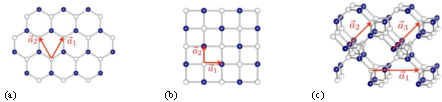
\includegraphics[width=\linewidth]{./chapter05/SublatticeSymmetry.pdf}
	\caption{
		Visualization of the A and B sublattices (in white and blue, respectively) for the (a) honeycomb, (b) square and (c) hyperhoneycomb lattices.
		While the sublattices of the honeycomb lattice have the same translation symmetry as the original lattice, the same is not true for the square and hyperoctagon lattices, leading to a non-vanishing $\bk_0$.
	}
	\label{fig:chapter05_Sublattices}
\end{figure}
%

As discussed in Chapters~\ref{chapter:KitaevHoneycombModel} and~\ref{chapter:ProjectiveSymmetryGroup}, the time-reversal operator in the Majorana sector must be supplemented by a gauge transformation $\op{G}_{\mathcal{T}}$ in order to yield a time-reversal symmetric \textit{Ansatz}.
The required gauge transformation has already been shown to be the sublattice transformation discussed above, \ie, it is specified by the (potentially) spatially-dependent gauge transformation
%
\begin{equation}
	G_{\mathcal{T}}(\br, \alpha) = \zeta_{\alpha}(\br).
\end{equation}
%
The presence of time-reversal symmetry enforces the momentum-space relations
%
\begin{equation}
	\begin{matrix*}[l]
		H(\bk) = G\dag_{\mathcal{T}}~H^*(-\bk + \bk_0)~G_{\mathcal{T}} \\
		\\
		E_{\alpha}(\bk) = E_{\beta}(-\bk + \bk_0),
	\end{matrix*}
\end{equation}
%
where $G_{\mathcal{T}}$ corresponds to a matrix representation of the gauge transformation $\op{G}_{\mathcal{T}}$ which acts on the entire unit cell, implying that the Majorana spectrum is symmetric under inversion through the point $\bk_0$.
Note that in a typical fermionic system, the time-reversal operation relates states at $\bk$ to $-\bk$, whereas the projective representation required for the gauge theory here is distinct in that it relates states at $\bk$ to $-\bk + \bk_0$.
Due to the general fact that time-reversal symmetry is the combination of particle-hole and sublattice symmetries and the fact that particle-hole symmetry is \textit{always} present in the gauge theory for the Kitaev model, both sublattice and time-reversal symmetries must always be broken simultaneously, \ie, the breaking of one implies the breaking of the other.


\textit{Inversion symmetry}:
Several lattices considered in this chapter possess inversion centers, resulting in spin liquid ground states with an inversion symmetry.
In general, the projective representation of the inversion operator has an associated gauge transformation $\op{G}_{\mathcal{P}}$.
In many cases this operator is trivial in the sense that it does not vary in space.
However, in certain cases the required gauge transformation is spatially-dependent.
Similar to the sublattice transformation, it may possess an overall sign factor which oscillates with wave vector $\til{\bk}_0 = (m_1 \bq_1 + m_2 \bq_2 + m_3 \bq_3)/2$ ($m_i \in \{0, 1\}$) as
%
\begin{equation}
	G_{\mathcal{P}}(\br, \alpha) = e^{i \til{\bk}_0 \cdot \br} G_{\mathcal{P}} (\bm{0}, \alpha).
\end{equation}
%
Note that the wave vector $\til{\bk}_0$ is distinct from the wave vector $\bk_0$ associated to time-reversal and sublattice symmetries.

The presence of inversion symmetry, thus, implies the momentum space relationships
%
\begin{equation}
	\begin{matrix*}[l]
		H(\bk) = G\dag_{\mathcal{P}}~U_{\mathcal{P}}~H(-\bk + \til{\bk}_0)~U\dag_{\mathcal{P}}~G_{\mathcal{P}} \\
		\\
		E_{\alpha}(\bk) = E_{\beta}(-\bk + \til{\bk}_0),
	\end{matrix*}
\end{equation}
%
where $U_{\mathcal{P}}$ and $G_{\mathcal{P}}$ are the matrix representations of the inversion operation $\op{\mathcal{P}}$ and the associated gauge transformation $\op{G}_{\mathcal{P}}$, respectively, which act on the entire unit cell.
The above relations imply that the Majorana spectrum is symmetric under inversion through the point $\til{\bk}_0$.
Note that in a typical fermionic system, the inversion operation relates states at $\bk$ to $-\bk$, whereas the projective representation required for the gauge theory here is distinct in that it relates states at $\bk$ to $-\bk + \til{\bk}_0$.


\textit{Effects of projective symmetries on the Majorana spectrum}:
In Section~\ref{section:chapter05_3DKitaevModels}, the Kitaev honeycomb model is extended to a number of three-dimensional, tricoordinated lattices.
In all cases, the ground state of the Kitaev Hamiltonian is a \ZZ~quantum spin liquid with gapped flux excitations.
Analogous to what is seen to occur on the honeycomb lattice in Chapter~\ref{chapter:KitaevHoneycombModel} for roughly isotropic exchange couplings, excitations above the spin liquid ground state are gapless fermions.
However, whereas in the case of the honeycomb lattice the excitations correspond to 2D Dirac fermions, the low-energy physics for the other lattices considered varies greatly, as can be seen in the overview of results provided in Table~\ref{table:chapter05_MajoranaSpectrumOverview}.
%
\begin{table}[tb]
	\centering
	\begin{tabular*}{\linewidth}{@{\extracolsep{\fill}}l|cc}
		\multirow{2}{*}{Lattice} & \multicolumn{2}{c}{Majorana spectrum} \\
		& Pure Kitaev    & TRS breaking         \\
		\hline\hline
		(10,3)a					 & Fermi surface  & Fermi surface        \\
		(10,3)b 				 & Nodal line     & Weyl nodes           \\
		(10,3)c 				 & Nodal line     & Fermi surface        \\
		\hline
		(9,3)a$^*$ 				 & Weyl nodes     & Weyl nodes           \\
		\hline
		(8,3)a  				 & Fermi surface  & Fermi surface        \\
		(8,3)b  				 & Weyl nodes     & Weyl nodes           \\
		(8,3)c$^*$ 				 & Nodal line     & Weyl nodes           \\
		(8,3)n  				 & Gapped         & Weyl nodes           \\
		\hline
		(6,3)  					 & Dirac nodes    & Gapped (non-Abelian)
	\end{tabular*}
	\caption{
		Overview of the Majorana spectrum for three-dimensional Kitaev models.
		Shown is a characterization of the nodal structure of the metallic states formed by the itinerant Majorana fermions in the gapless spin liquid phase of three-dimensional Kitaev models defined on the tricoordinated lattices of Table~\ref{table:chapter05_LatticeOverview}.
		Results for the pure Kitaev model are given in the second column.
		The third column provides information on how the nodal structure changes in the presence of an explicit time-reversal symmetry (TRS) breaking magnetic field term.
		The asterisk indicates that for these two lattices, the ground state flux sector was not used for the calculation (for details see Sections~\ref{section:chapter05_8_3c} and~\ref{section:chapter05_9_3a}).
	}
	\label{table:chapter05_MajoranaSpectrumOverview}
\end{table}
%

Although the presence or absence of individual lattice symmetries plays a role in determining the properties of the gapless excitations, it is seen to be the projective representation of those symmetries which ultimately determines the low-energy structure of the theory.
As an example, lattices (10,3)b and (8,3)b both possess sublattice and inversion symmetries, however, it is ultimately the \textit{differing} projective representations of the respective time-reversal operators which lead to lattice (10,3)b hosting a one-dimensional nodal line while lattice (8,3)b hosts isolated, topological nodal points called \textit{Weyl nodes}.
Similarly, chiral lattices (10,3)a and (10,3)c both possess sublattice symmetry but lack inversion symmetry.
However, the differing projective representations of the time-reversal operators lead to lattice (10,3)a hosting a full two-dimensional Fermi surface, whereas lattice (10,3)c hosts a one-dimensional nodal line.

The goal of this project was to determine the projective symmetry groups of the Kitaev spin liquids on a number of three-dimensional lattices corresponding to the symmetry group $SG = \avg{\{ \op{T}_1, \op{T}_2, \op{T}_3, \op{\mathcal{P}}, \op{\mathcal{T}} \}}$ and use that information to classify them according to their different PSG-protected Majorana Fermi surface topologies.
The symmetry group used in this work was chosen to represent what the authors considered to be the most fundamental symmetries and was thought to provide a complete classification of the Kitaev spin liquids.

With the benefit of hindsight and a better understanding of the ideas behind the projective symmetry group, it becomes clear that the \textit{entire} symmetry group for a given lattice should be taken into account.
Reference~\cite{YamadaPRB2017} examined Kitaev spin liquids on the three-dimensional tricoordinated lattices $8^{2}.10$-a and (10,3)d, which were not considered in the work detailed here.
Lattice $8^{2}.10$-a was shown to host a pair of three-dimensional Dirac nodes protected by a combination of fourfold-screw and and glide symmetries.
The spin liquid of lattice (10,3)d exhibits a pair of linked nodal lines protected by a combination of time-reversal and glide symmetries, one of which is stable even after time-reversal symmetry is broken.
Furthermore, Chapter~\ref{chapter:HypernonagonLattice} provides a more accurate and detailed analysis of lattice (9,3)a wherein the lattice is seen to host a nodal line phase protected by a combination of inversion and time-reversal symmetries, both of which are absent individually.
All of these possibilities are overlooked by the choice of symmetry group used here and the choice of lattices which, by chance rather than design, did not challenge such a classification scheme.

Having said that, the specific method of classification detailed here is still valid for many cases and at the very least serves to illustrate the power of the projective symmetry group as well as the richness of the physics of Kitaev spin liquids.
Many of the lattices considered here were introduced in the context of quantum magnetism for the first time through this work and it has served as a springboard for research on a variety of gapless spin liquids which had not been previously seen.

Rather than try to explain the systematic determination of Table~\ref{table:chapter05_MajoranaSpectrumOverview} in this section without the proper context, the individual ideas are explained in the next section as they become relevant.
In Section~\ref{section:chapter05_Conclusion} these principles are summarized as a coherent classification scheme.

%
\begin{figure}[p]
	\centering
	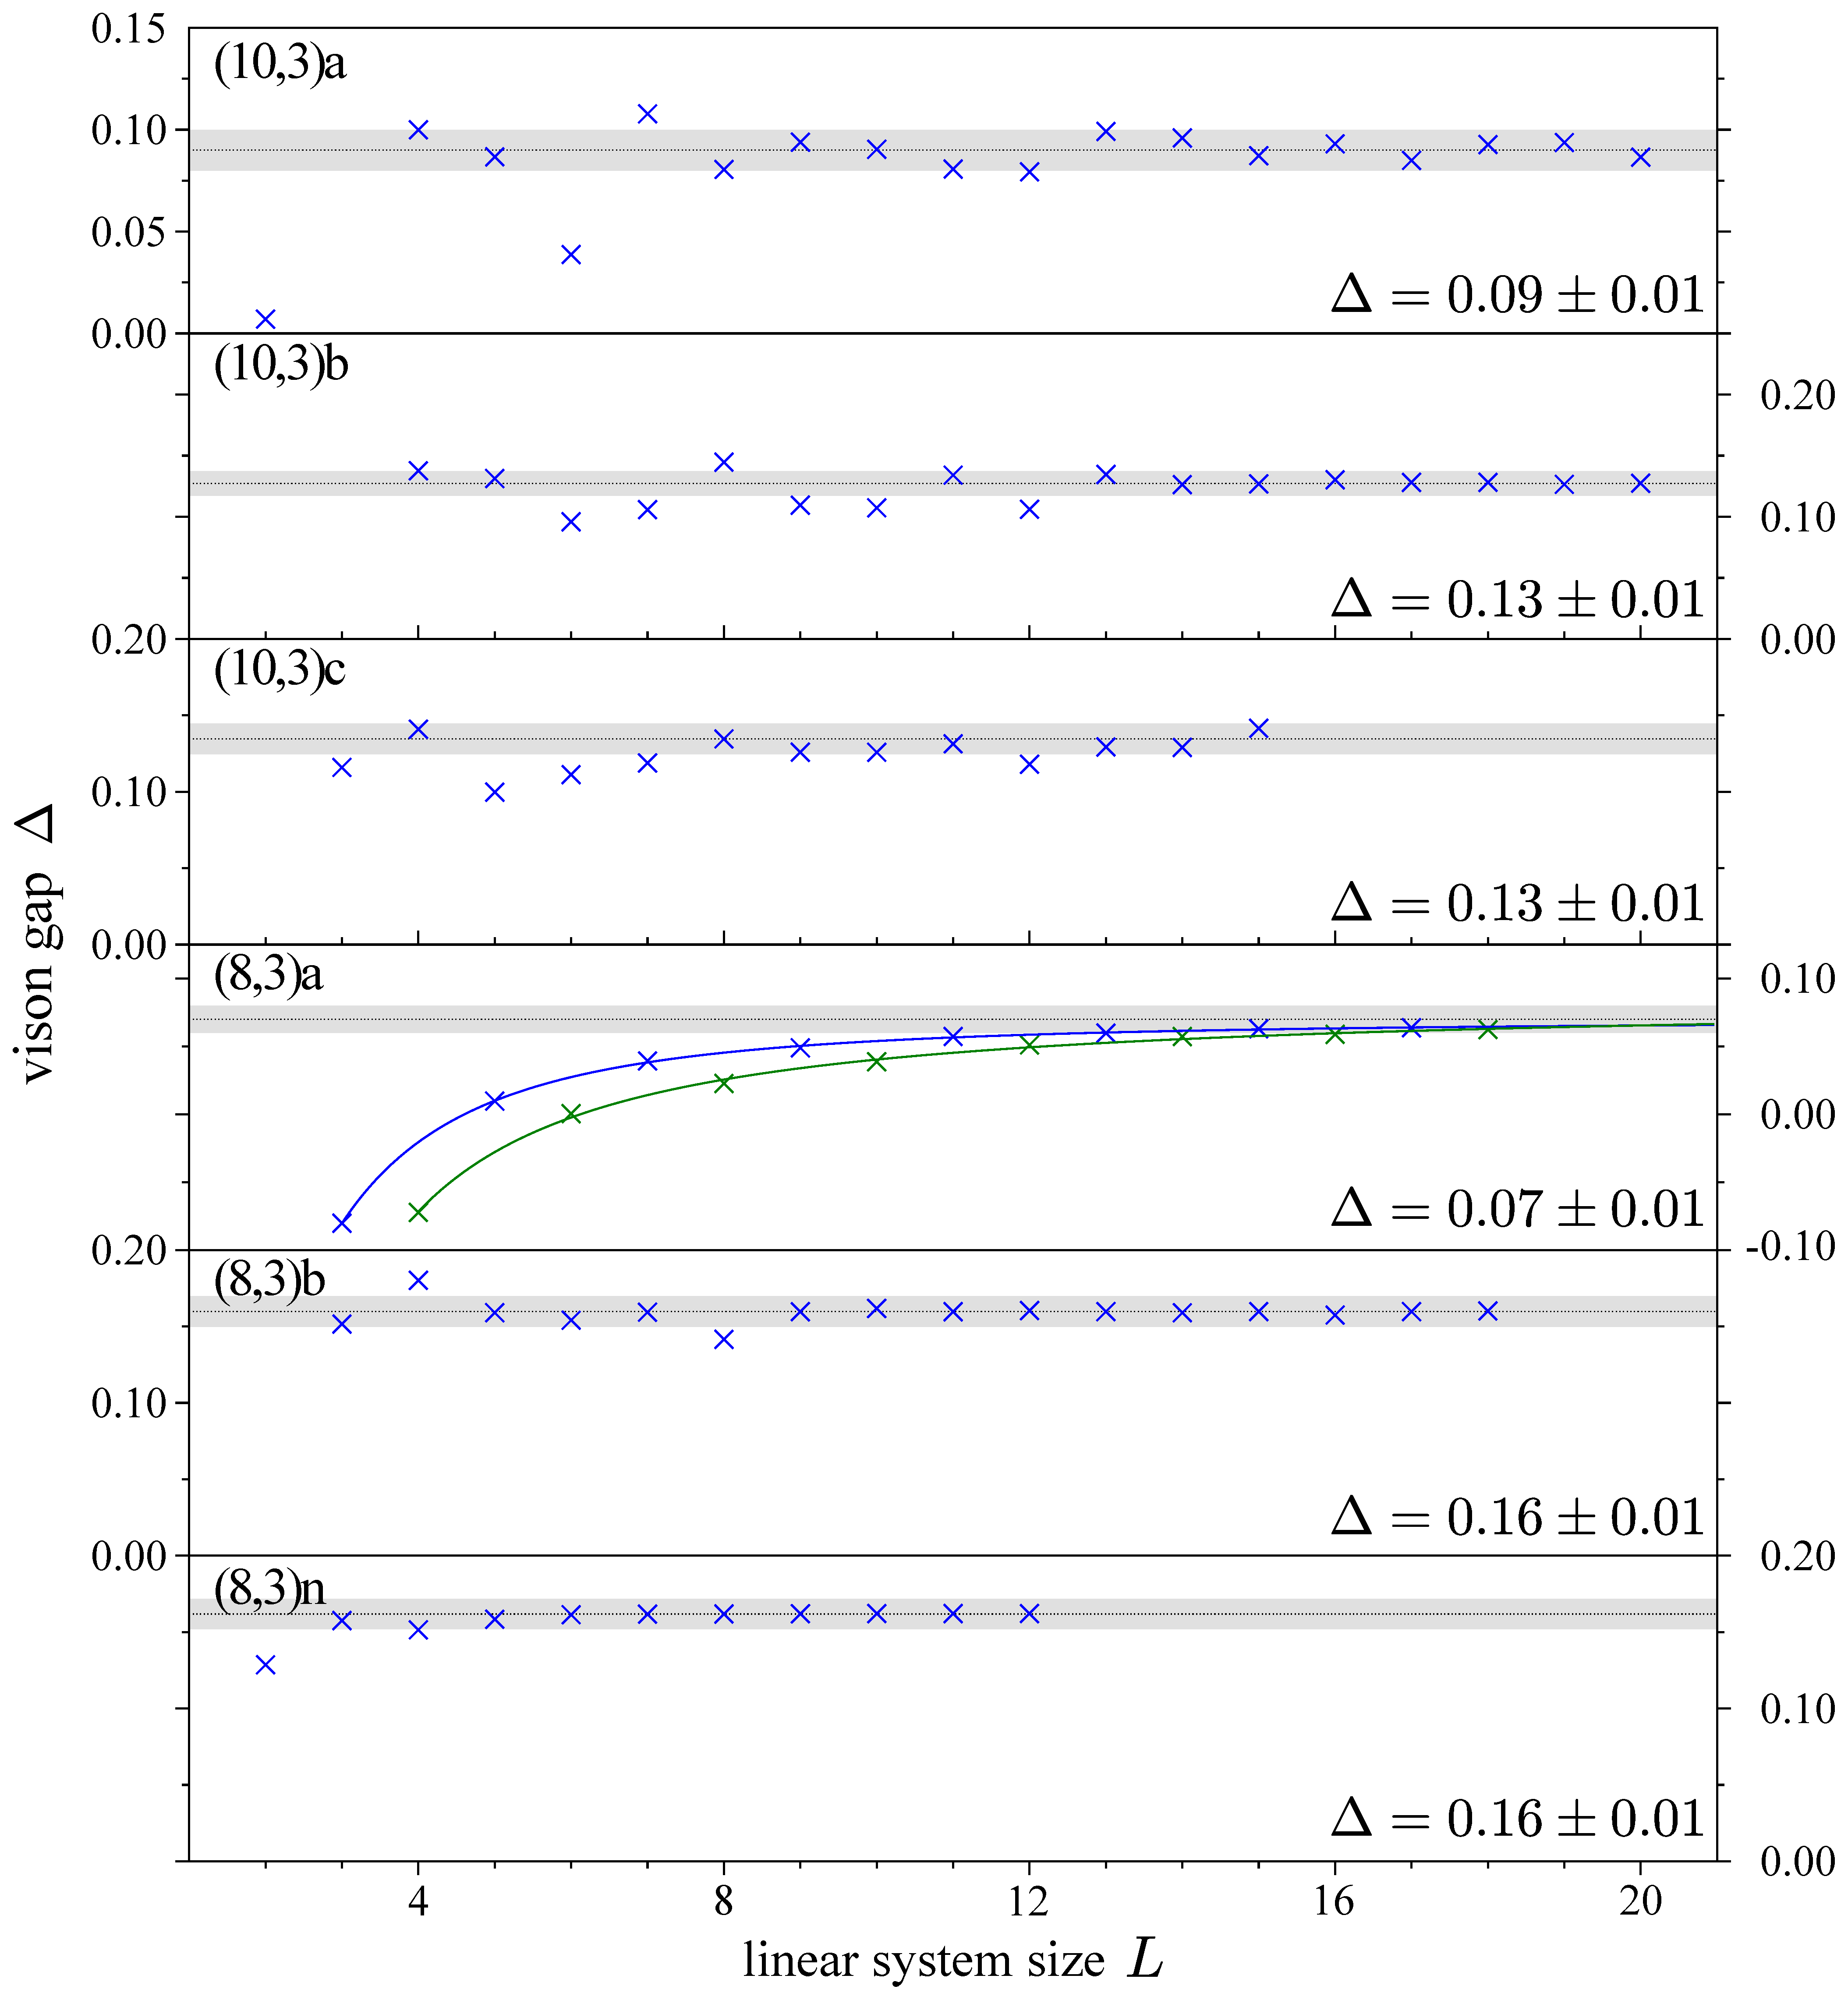
\includegraphics[width=0.95\linewidth]{./chapter05/VisonGap.pdf}
	\caption{
		Vison gap at the isotropic point obtained for the smallest vison loop as a function of system size.
		The dotted line marks the extrapolation of the gap for infinite system size, and the gray bar denotes the error of the extrapolation.
		Energies expressed in units of the exchange coupling at the isotropic point.
		Details on the vison loops can be found in Appendix~\ref{appendix:ThreeDimensionalKitaevModels}.
	}
	\label{fig:chapter05_VisonGaps}
		
	\vspace{0.5cm}

	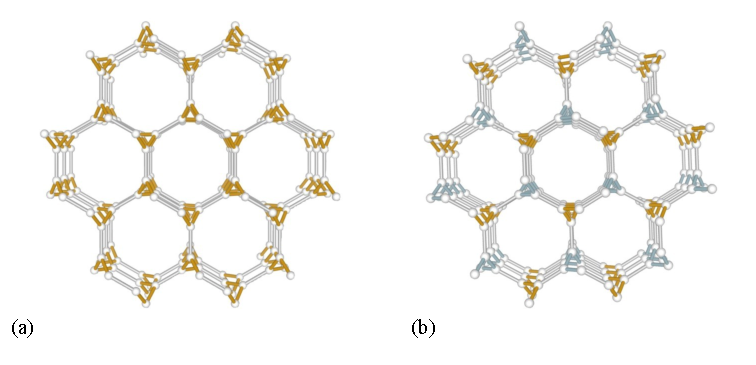
\includegraphics[width=0.7\linewidth]{./chapter05/8_3abComparison.pdf}
	\caption{
	Comparison of the co- and counter-rotating spirals of lattices (8,3)a and (8,3)b, respectively.
	The two different rotation directions are indicated by orange and blue.
	}
	\label{fig:chapter05_8_3abComparison}
\end{figure}
%

%
%\begin{figure}[p]
%	\centering
%	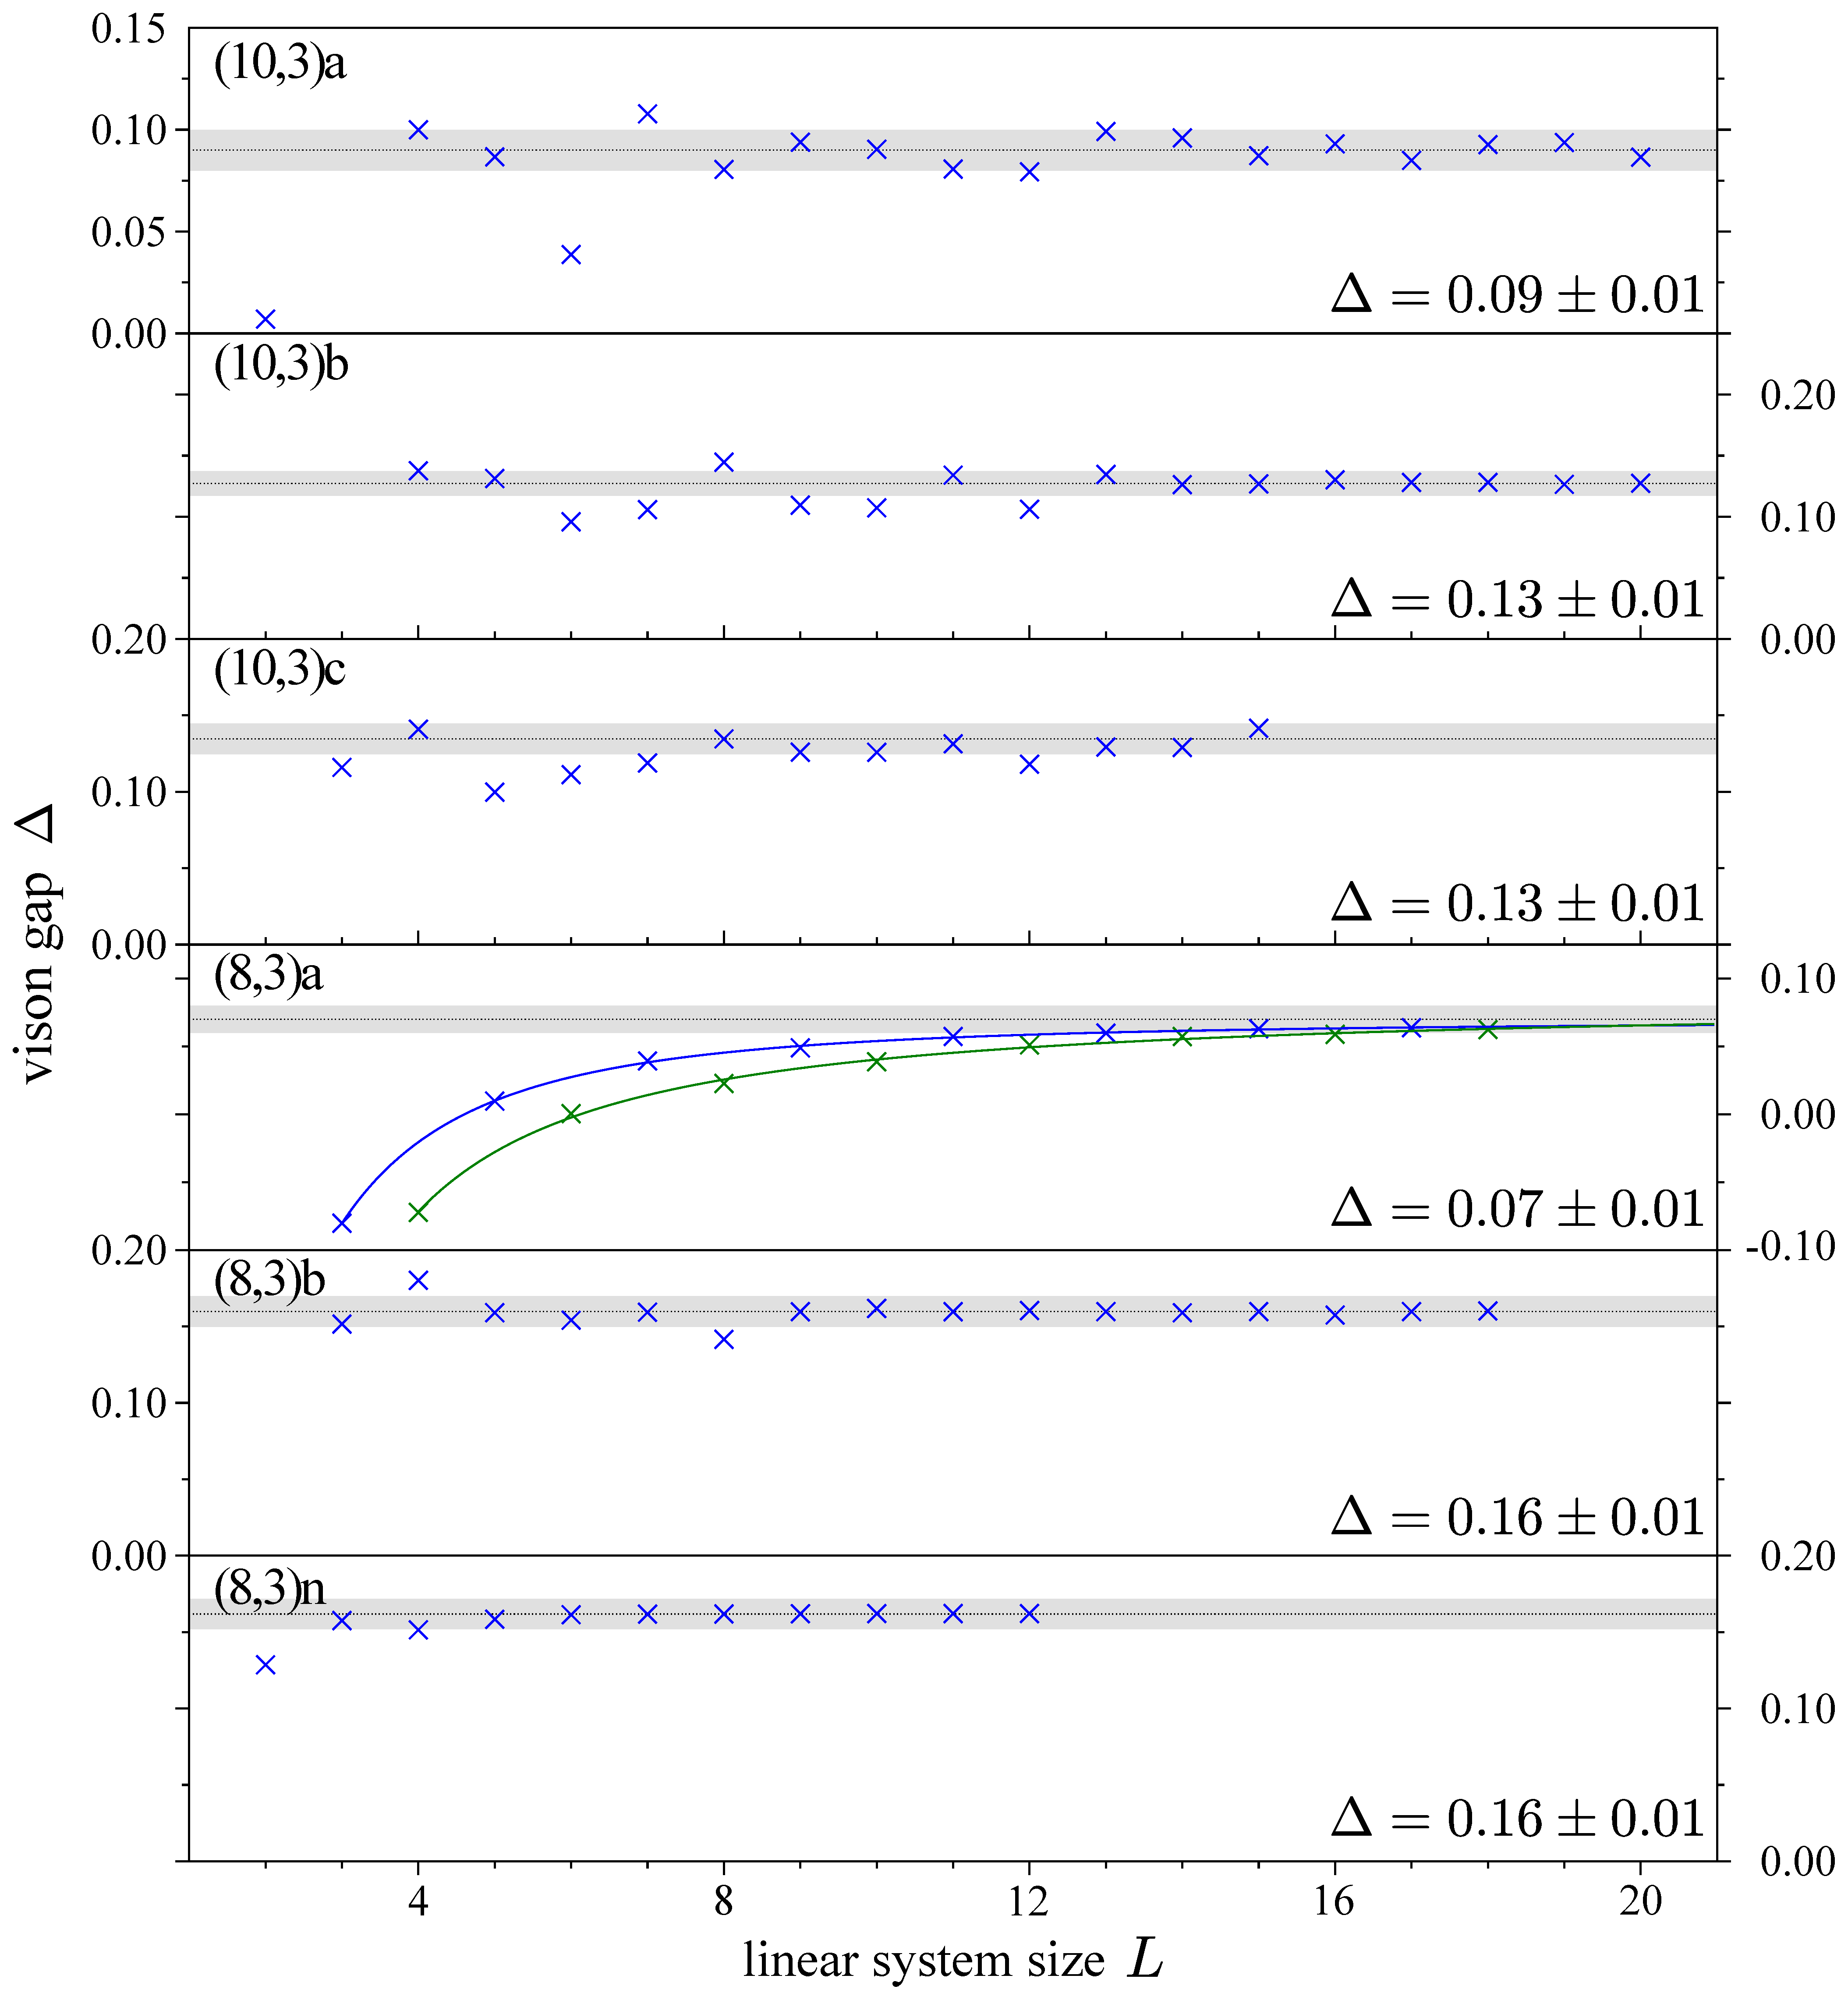
\includegraphics[width=\linewidth]{./chapter05/VisonGap.pdf}
%	\caption{
%		Vison gap obtained for the smallest vison loop as a function of system size.
%		The dotted line marks the extrapolation of the gap for infinite system size, and the gray bar denotes the error of the extrapolation.
%		Details on the vison loops can be found in Appendix~\ref{appendix:ThreeDimensionalKitaevModels}.
%	}
%	\label{fig:chapter05_VisonGaps}
%\end{figure}
%
%
%\begin{figure}[tb]
%	\centering
%	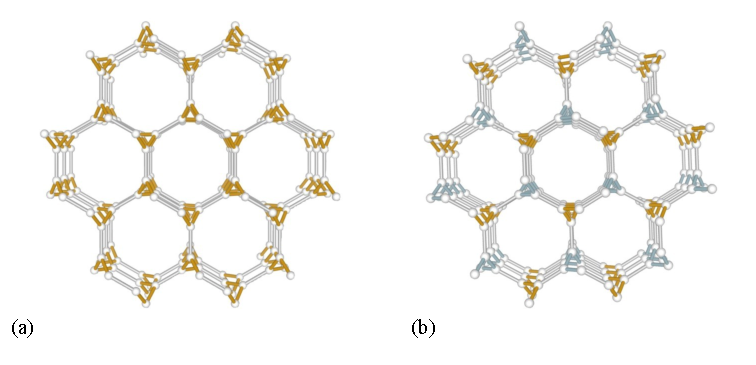
\includegraphics[width=0.8\linewidth]{./chapter05/8_3abComparison.pdf}
%	\caption{
%		Comparison of the co- and counter-rotating spirals of lattices (8,3)a and (8,3)b, respectively.
%		The two different rotation directions are indicated by orange and blue.
%	}
%	\label{fig:chapter05_8_3abComparison}
%\end{figure}
%

%
%
%%%%%%%%%%%%%%%%%%%%%%%%%%%%%%%%%%%%%%%%%%%%%%%%%%%%%%%%%%%%%%%%%%%%%%%%%%%%%%%%%%%%%%%%
\section{3D Kitaev models}
\label{section:chapter05_3DKitaevModels}
%%%%%%%%%%%%%%%%%%%%%%%%%%%%%%%%%%%%%%%%%%%%%%%%%%%%%%%%%%%%%%%%%%%%%%%%%%%%%%%%%%%%%%%%
%
%
This section introduces a number of three-dimensional tricoordinated lattices on which a Kitaev model shall be defined and provides a thorough analysis of the corresponding \ZZ~spin liquid ground state in the gapless regime.
Each lattice has a subsection dedicated to it following roughly the same pattern.
Each subsection begins by providing some elementary information about the lattice structure and the assignment of Kitaev couplings to it.
Next, the gauge structure of the corresponding gauge theory is discussed including information about the fundamental loops\footnote{Note the difference between \textit{fundamental} and \textit{elementary} loops in this context as it differs from the nomenclature of previous chapters. Here, \textit{elementary} loops are defined as the smallest closed loops in the lattice. These define the polygonality of the lattice. The \textit{fundamental} loops are defined as the smallest set of closed loops from which all other loops in the lattice may be constructed.}~of the lattice and the assignment of \ZZ~fluxes in the ground state.
What follows is a determination of the projective symmetry group and the restrictions it places on the Majorana spectrum.
Finally, a detailed analysis of the gapless Majorana spectrum is carried out.
For a brief overview of the lattices, refer to Table~\ref{table:chapter05_LatticeOverview}.
%
\begin{table}[tb]
	\centering
	\begin{tabular*}{\linewidth}{l|@{\extracolsep{\fill}}ccccc}
		Lattice 	& Sites in  & Sublattice          & Inversion                 & \multicolumn{2}{c}{Space group} \\
		& unit cell & symmetry  & symmetry            & Symbol               	  & No.      \\
		\hline\hline
		(10,3)a 	& 4         & $\bk_0 \neq \bm{0}$ & chiral                    & I$4_1 32$            & 214      \\
		(10,3)b 	& 4         & \checkmark          & \checkmark                & Fddd                 & 70       \\
		(10,3)c 	& 6         & \checkmark          & chiral                    & P$3_1 12$            & 151      \\
		\hline
		(9,3)a  	& 12        & ---                 & \checkmark                & R$\overline{3}$m     & 166      \\
		\hline
		(8,3)a  	& 6         & $\bk_0 \neq \bm{0}$ & chiral                    & P$6_2 22$            & 180      \\
		(8,3)b  	& 6         & $\bk_0 \neq \bm{0}$ & \checkmark                & R$\overline{3}$m     & 166      \\
		(8,3)c  	& 8         & \checkmark          & \checkmark                & P$6_3$ / mmc         & 194      \\
		(8,3)n  	& 16        & \checkmark          & $\til{\bk}_0 \neq \bm{0}$ & I4 / mmm             & 139      \\
		\hline
		(6,3)   	& 2         & \checkmark          & \checkmark                &                      &         
	\end{tabular*}
	\caption{
		Overview of elementary tricoordinated lattices in (mostly) three spatial dimensions.
		Following the classification of A.~F. Wells~\cite{Wells1977}, the lattices considered here are of fixed polygonality $p$, \ie, a fixed length of all elementary closed loops, and vertex coordination $c=3$ using the Schl\"afli symbol $(p,c)$ followed by a letter.
		Basic information is listed for each lattice including the number of lattice sites $Z$ in the unit cell, whether the lattice exhibits (non-trivial) sublattice and/or inversion symmetries, as well as information about the space group.
	}
	\label{table:chapter05_LatticeOverview}
\end{table}
%


%
%
% LATTICE (8,3)A %%%%%%%%%%%%%%%%%%%%%%%%%%%%%%%%%%%%%%%%%%%%%%%%%%%%%%%%%%%%%%%%%%%%%%%
\subsection{Lattice (8,3)a}
\label{section:chapter05_8_3a}
%%%%%%%%%%%%%%%%%%%%%%%%%%%%%%%%%%%%%%%%%%%%%%%%%%%%%%%%%%%%%%%%%%%%%%%%%%%%%%%%%%%%%%%%
%
%
\subsubsection{Lattice information}
%
%
The first lattice to be considered is (8,3)a.
The lattices (8,3)a and (8,3)b (Section~\ref{section:chapter05_8_3b}) are, in a sense, related.
Both may be viewed as a three-dimensional version of the 3-12-12~\cite{YangPRB2007} or Yao-Kivelson lattice~\cite{YaoPRL2007}, with the triangles replaced by triangular spirals.
Whereas the spirals of lattice (8,3)a are co-rotating, resulting in a chiral lattice, those of lattice (8,3)b are counter-rotating, yielding an inversion-symmetric lattice (refer to Figure~\ref{fig:chapter05_8_3abComparison} for a comparison).

More formally, lattice (8,3)a is specified by the hexagonal space group $P6_{2}22$ (No. 180) with $c/a = 3\sqrt{2}/5$ and Wyckoff positions for the unit cell are $6(i)$ with $x=2/5$.
The concrete choice of six site unit cell used in this work is given by the site positions
%
\begin{equation}
	\begin{matrix*}[l]
		\br_1 = \left(\frac{1}{2}, \frac{\sqrt{3}}{10}, 0\right) &
		\br_2 = \left(\frac{3}{5}, \frac{\sqrt{3}}{5}, \frac{2\sqrt{2}}{5}\right) &
		\br_3 = \left(\frac{1}{10}, \frac{3\sqrt{3}}{10}, \frac{\sqrt{2}}{5}\right) \\
		&\\
		\br_4 = \left(\frac{2}{5}, \frac{\sqrt{3}}{5}, \frac{\sqrt{2}}{5}\right) &
		\br_5 = \left(0, \frac{2\sqrt{3}}{5}, 0\right) &
		\br_6 = \left(-\frac{1}{10}, \frac{3\sqrt{3}}{10}, \frac{2\sqrt{2}}{5}\right).
	\end{matrix*}
\end{equation}
%
The lattice vectors are chosen to be
%
\begin{equation}
	\begin{matrix*}[l]
		\ba_1 = (1, 0, 0) \qquad
		\ba_2 = \left(-\frac{1}{2}, \frac{\sqrt{3}}{2}, 0\right) \qquad
		\ba_3 = \left(0, 0, \frac{3\sqrt{2}}{5}\right)
	\end{matrix*}
\end{equation}
%
with the corresponding reciprocal lattice vectors
%
\begin{equation}
	\begin{matrix*}[l]
		\bq_1 = \left(2\pi, \frac{2\pi}{\sqrt{3}}, 0\right) \qquad
		\bq_2 = \left(0, \frac{4\pi}{\sqrt{3}}, 0\right) \qquad
		\bq_3 = \left(0, 0, \frac{5\sqrt{2}\pi}{3}\right).
	\end{matrix*}
\end{equation}
%

The unit cell and translation vectors are illustrated in Figure~\ref{fig:chapter05_8_3aPanel}~(a).
The bonds in the figure are colored red, green and blue to indicate the assignment of $x$-, $y$- and $z$-type bonds, respectively.
This assignment of bonds is chosen to respect as many of the lattice symmetries as possible and is unique up to an overall permutation of the three bond types.
More specifically, there are two distinct sets of $x$-, $y$- and $z$-bonds which cannot be related by symmetries, namely, those which compose the co-rotating spirals and those which connect neighboring spirals.
All bonds in a given set, however, are related by a combination of a $C_2$ rotation and a threefold screw axis.
The symmetry between $x$-, $y$- and $z$-bonds is reflected in the ground state phase diagram shown in Figure~\ref{fig:chapter05_8_3aPanel}~(b).


%
%
\subsubsection{Gauge structure}
%
%
Lattice (8,3)a possesses three loop operators of length 8 and three of length 14 per unit cell.
These six loop operators may be combined to form three closed volumes leading to only \textit{three} independent loop operators per unit cell (see Appendix~\ref{appendix:ThreeDimensionalKitaevModels_8_3a} for details).
The canonical flux sector for lattice (8,3)a corresponds to $\pi$-flux through all loops of length 8 and $0$-flux through all loops of length 14.
This results in all loop operators $\op{W}_p$ having eigenvalue +1.
Additionally, it has been checked numerically that the canonical flux sector is, indeed, the ground state flux sector.
The vison gap for lattice (8,3)a shown in Figure~\ref{fig:chapter05_VisonGaps}~and Table~\ref{table:chapter05_VisonGaps}~has been computed by flipping the value of $u_{jk}$ for a single $z$-bond, resulting in the excitation of four loop operators (further details are given in Appendix~\ref{appendix:ThreeDimensionalKitaevModels_8_3a}).
%
\begin{table}[tb]
	\centering
	\begin{tabular*}{\linewidth}{l|@{\extracolsep{\fill}}ccc}
		Lattice     & Flux sector    & Vison gap & Vison loop length \\
		\hline\hline
		(10,3)a     & $0$-flux       & 0.09(1)   & 10                \\
		(10,3)b     & $0$-flux       & 0.13(1)   & 6                 \\
		(10,3)c     & $0$-flux       & 0.13(1)   & 3                 \\
		\hline
		(9,3)a$^*$  & $\pi/2$-fluxes & ---       & 4                 \\
		\hline
		(8,3)a      & $\pi$-flux     & 0.07(1)   & 2                 \\
		(8,3)b      & $\pi$-flux     & 0.16(1)   & 2                 \\
		(8,3)c$^*$  & $0$-flux       & ---       & 4                 \\
		(8,3)n      & $\pi$-flux     & 0.16(1)   & 2                 \\
		\hline
		(6,3)       & $0$-flux       & 0.27      & ---                
	\end{tabular*}
	\caption{
		Overview of the physics of the \ZZ~gauge field for three-dimensional Kitaev models.
		The second column provides the flux assignment of the \textit{elementary} loops for the Kitaev model defined on the lattices in the first column.
		The third column gives the size of the vison gap for isotropic couplings in units of the exchange coupling, whereas the fourth column provides the length of the smallest vison loop in terms of the number of excited \textit{elementary} loop operators.
		The asterisk indicates that for these two lattices, the results provided do not correspond to the ground state flux sector.
	}
	\label{table:chapter05_VisonGaps}
\end{table}
%


%
%
\subsubsection{Projective symmetries}
%
%
Lattice (8,3)a is bipartite with different sublattices connected by the vector $\br_0 = \ba_3$.
As a result, the projective representation of time-reversal is given by
%
\begin{equation}
	H(\bk) = G\dag_{\mathcal{T}}~H(-\bk + \bk_0)~G_{\mathcal{T}},
\end{equation}
%
where $\bk_0 = \bq_3/2$ and the associated gauge transformation matrix is given by
%
\begin{equation}
	G_{\mathcal{T}} =
		\begin{pmatrix}
			\id & 0 \\
			0	& -\id
		\end{pmatrix}.
\end{equation}
%
As lattice (8,3)a is chiral, the only other restriction to consider is that of particle-hole symmetry.
The resulting energy relations are given by\pagebreak
%
\begin{equation}
	E_{\alpha}(\bk) = -E_{\beta}(-\bk) \qquad {\rm and } \qquad E_{\alpha}(\bk) = E_{\gamma}(-\bk + \bk_0),
\end{equation}
%
due to particle-hole and time-reversal symmetry, respectively.
Due to the fact that the gauge transformation $\op{G}_{\mathcal{T}}$ relates states at momentum $\bk$ to states at momentum $\bk - \bk_0$, the momentum space Hamiltonian matrix has the general form
%
\begin{equation}
	H(\bk) = 
		\begin{pmatrix}
			0			&			& A(\bk) 	\\
						& \ddots 	& 			\\
			A\dag(\bk)	&			& 0
		\end{pmatrix},
	\label{eq:chapter05_8_3aGenericHamiltonian}
\end{equation}
%
\ie, other than being skew-symmetric (due to the Majorana condition), it is a generic band Hamiltonian.


%
%
\subsubsection{Majorana band structure}
%
%
Given the general form of the Kitaev Hamiltonian in Eq.~\eqref{eq:chapter05_8_3aGenericHamiltonian} for lattice (8,3)a, zero modes at a given momentum correspond to a vanishing determinant of the Hamiltonian matrix $H(\bk)$.
In three-dimensions, solutions of $\det{H(\bk)} = 0$ correspond to a two-dimensional manifold of $\bk$-points.
The conclusion is that for the Kitaev model defined on lattice (8,3)a, the only stable zero-energy manifolds are \textit{Fermi surfaces}.

The fact that lattice (8,3)a has non-vanishing $\bk_0$ associated to the projective time-reversal operation while also lacking inversion symmetry implies the lack of an energy relation such as $E_{\alpha}(\bk) = -E_{\beta}(\bk)$.
A consequence of this lack of symmetry at a fixed momentum is that an isolated band may cross the Fermi energy, resulting in the formation of a Fermi surface.

Such a situation is even more interesting in the presence of degeneracies in the Majorana spectrum.
In the absence of symmetries, the spectrum of a generic band Hamiltonian may have degeneracies corresponding to bands $E_{+}(\bk)$ and $E_{-}(\bk)$ at isolated momenta $\bk^*$, described locally by
%
\begin{equation}
	E_{\pm} (\bk) \approx E_0(\bk^*) \pm \sum_i~b^{i}_{\pm} |k_{i} - k^*_{i}| \qquad {\rm where } \qquad b^{i}_{\pm} \in \mathbb{R}_{+}.
\end{equation}
%
For non-vanishing $E_0(\bk^*)$, the band $E_{-}$ may cross the Fermi energy resulting in a Fermi surface which may be gapped out only if the degeneracy is lifted.
Such a degeneracy is a topological property of the Hamiltonian with a robust topological charge (chirality) associated to it.
As such, these degeneracies may only be lifted by being brought into contact with another degeneracy of the opposite topological charge and mutually annihilating.\footnote{If interactions are allowed, however, degeneracies may be coupled non-locally in momentum space. Regardless, the interactions must couple degeneracies of opposite charge.}
Note that particle-hole symmetry guarantees the existence of a degeneracy with opposite topological charge located at $-\bk^*$ and with energy $E_0(-\bk^*) = -E_0(\bk^*)$.
As a result, the Fermi surface inherits a topological protection from the associated degeneracy.
Such degeneracies are closely related to the massless Weyl nodes which will be discussed in greater detail in Section~\ref{section:chapter05_8_3b}.
%
\begin{figure}[tb]
	\centering
	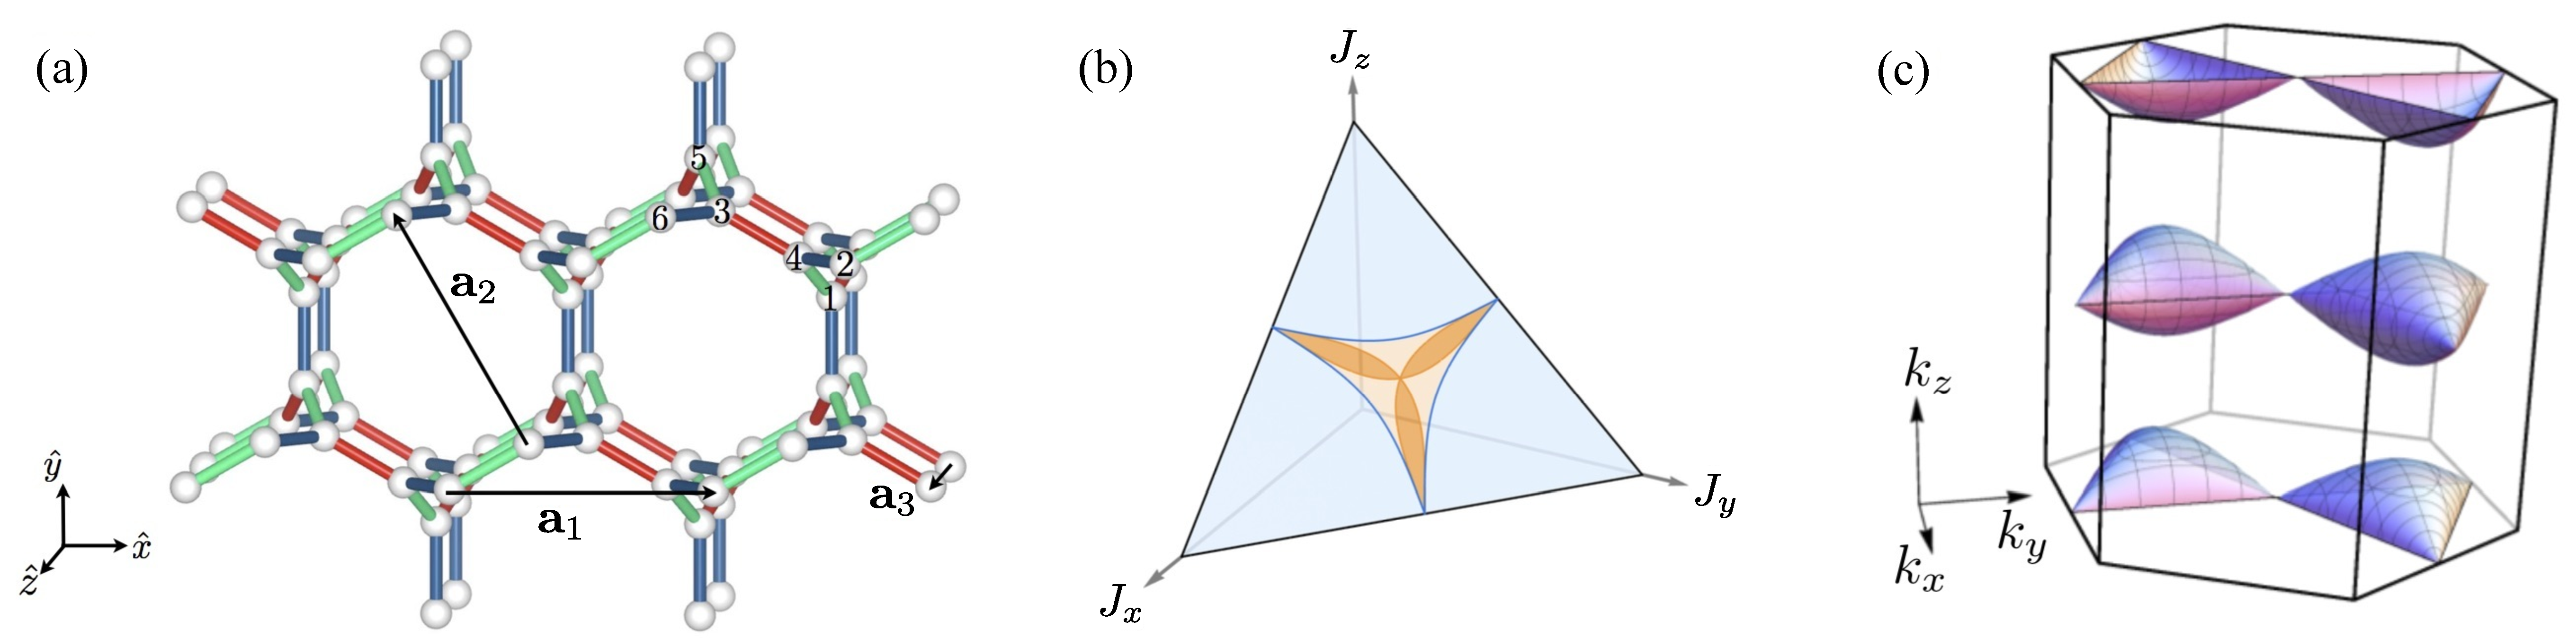
\includegraphics[width=\linewidth]{./chapter05/8_3aPanel.pdf}
	\caption{
		(a) Unit cell and translation vectors for the Kitaev model on lattice (8,3)a.
		(b) Ground state phase diagram for lattice (8,3)a.
		The regions shaded darker orange have topological Fermi surfaces while the lighter orange regions have topologically-trivial Fermi surfaces.
		The blue shaded regions are gapped.
		(c) Visualization of the four Majorana Fermi surfaces for isotropic exchange couplings.
	}
	\label{fig:chapter05_8_3aPanel}
\end{figure}
%

Diagonalizing the concrete Kitaev Hamiltonian for lattice (8,3)a reveals an extended gapless phase around the point of isotropic exchange couplings (see phase diagram in Figure~\ref{fig:chapter05_8_3aPanel}~(b)), where the zero modes correspond to the Majorana Fermi surfaces visualized in Figure~\ref{fig:chapter05_8_3aPanel}~(c).
The darker orange shaded regions of the phase diagram denote the parameter space where the Majorana Fermi surfaces are topologically protected, \ie, they are generated by a topological degeneracy as discussed above.
These degeneracies can be seen in the energy dispersion in Figure~\ref{fig:chapter05_8_3aDispersion}~(b).
For isotropic couplings, oppositely charged topological degeneracies are located at $\bk^* = \pm (\frac{\pi}{3}, \frac{\pi}{\sqrt{3}}, 0)$ and at $-\bk^* + \bk_0$ corresponding to their time-reversal partners.
Note that the act of time-reversal yields topological degeneracies of the \textit{same} charge and energy (see discussion of Weyl nodes in Section~\ref{section:chapter05_8_3b}).
Additionally, there are topologically neutral degeneracies located at the touching points of the different Fermi surfaces.
These topologically neutral points correspond to pairs of oppositely charged degeneracies sitting on top of one another.

As can be seen in Figure~\ref{fig:chapter05_8_3aPanel}~(c), pairs of Majorana Fermi surfaces are related by the nesting vector $\bk_0$, suggesting a Fermi surface instability for the case of \textit{interacting} Majorana fermions.
Interactions between Majorana fermions are introduced as soon as any other type of magnetic exchange is added to the pure Kitaev Hamiltonian, thus, such a possible instability becomes important for any realistic model.
A very similar situation occurs in the (10,3)a hyperoctagon lattice (see Section~\ref{section:chapter05_10_3a}) and was studied in Reference~\cite{HermannsPRL2015b}.
Details of this so-called \textit{spin-Peierls instability} are discussed in Section~\ref{section:chapter05_SpinPeierls}.
Breaking time-reversal symmetry by applying an external magnetic field does not qualitatively change the nature of the nodal manifold, \ie, they remain Fermi surfaces.
However, they do deform in a non-trivial way as magnetic field strength is varied, destroying the perfect nesting condition.\newpage
%
\begin{figure}[tb]
	\centering
	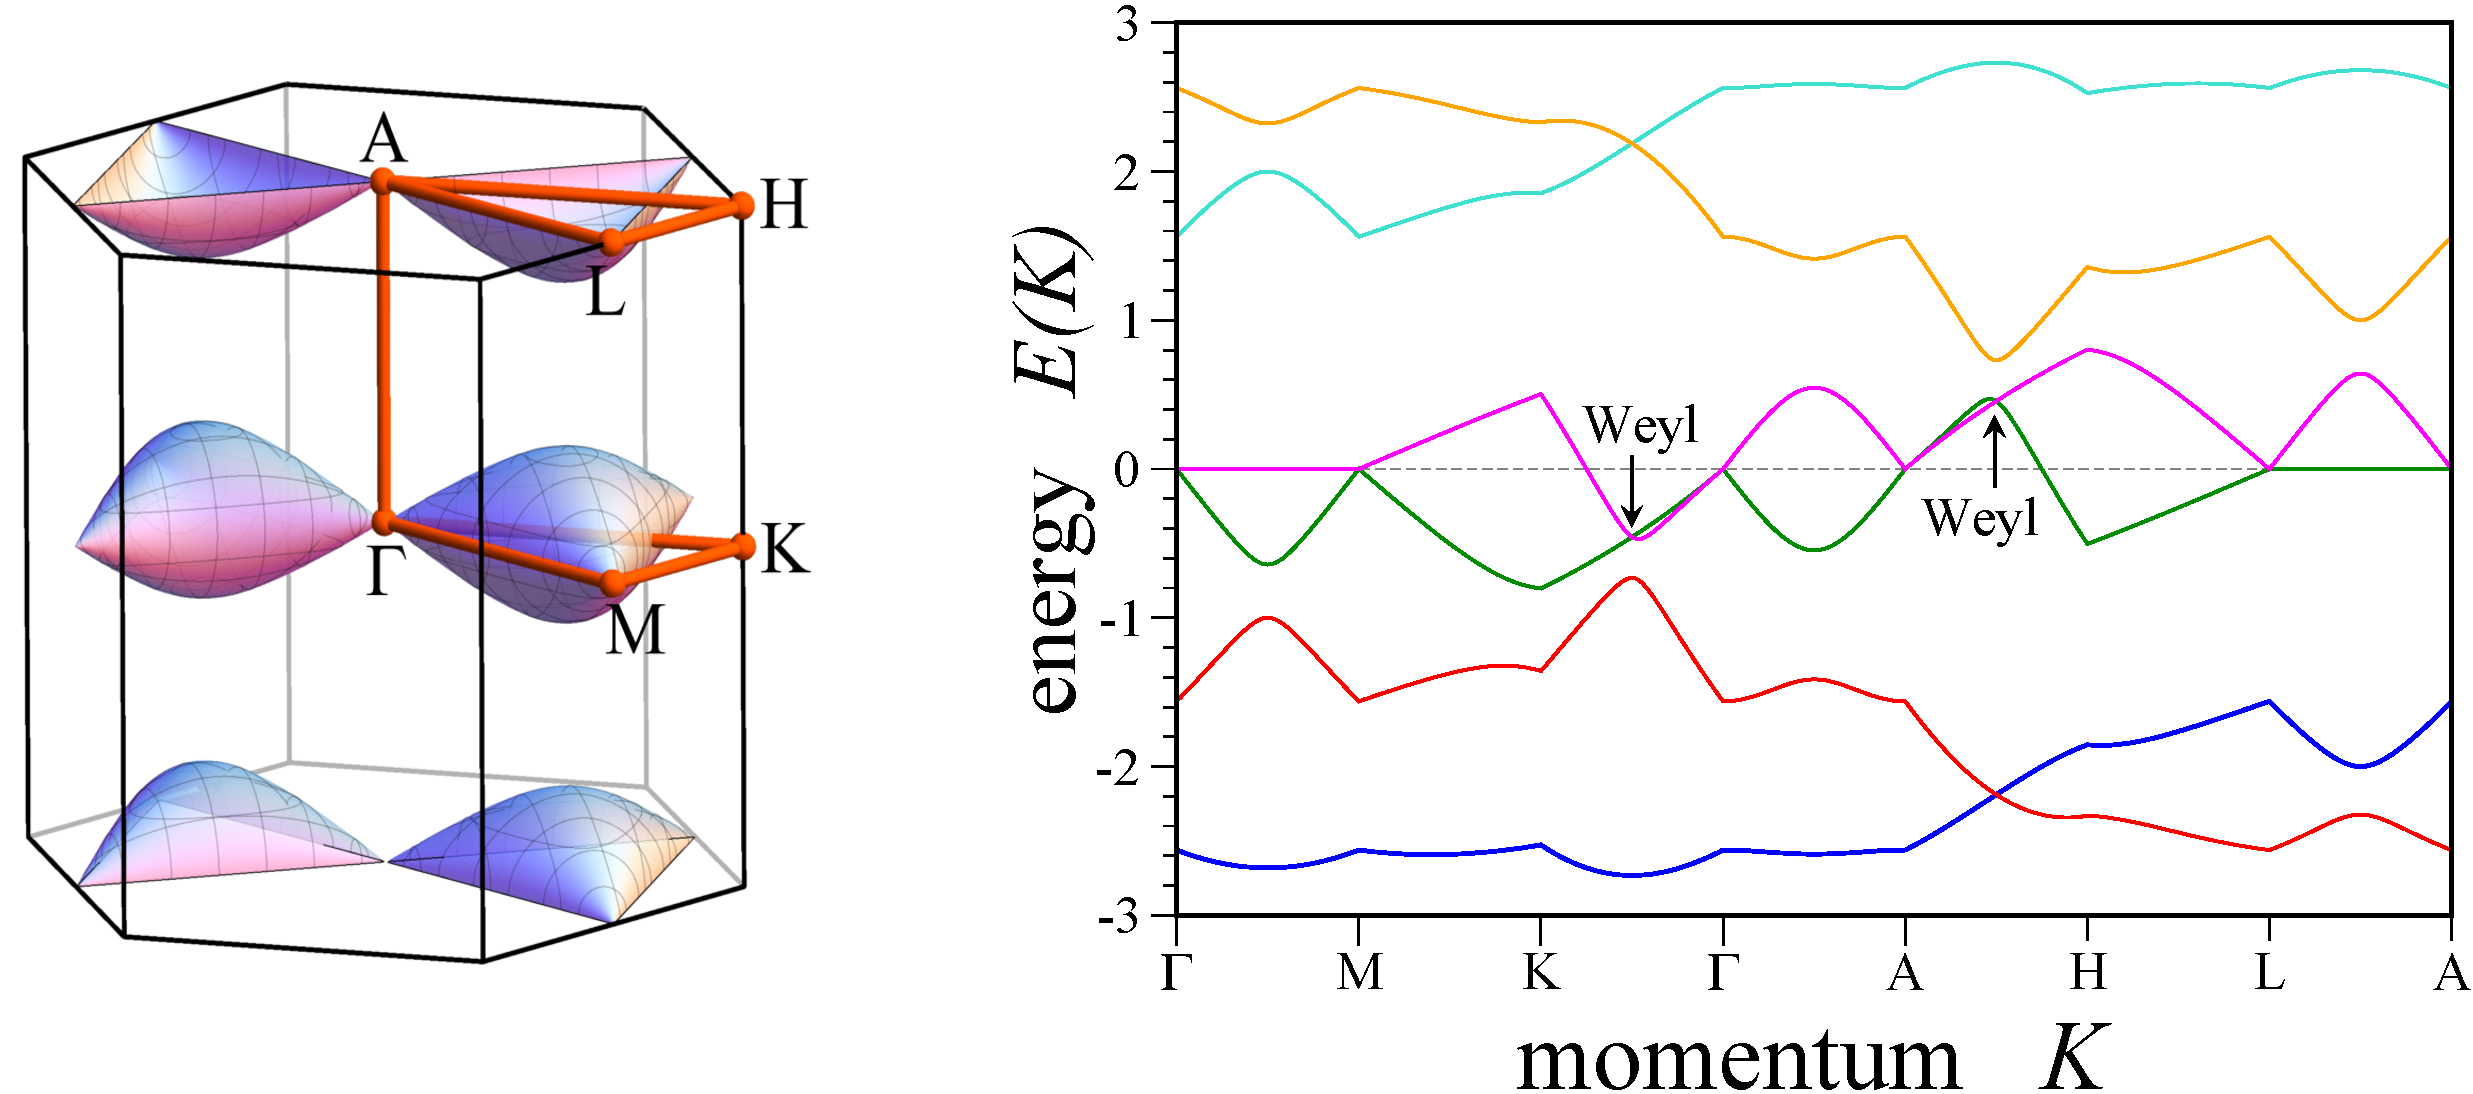
\includegraphics[width=\linewidth]{./chapter05/8_3aDispersion.pdf}
	\caption{
		(a) Brillouin zone of lattice (8,3)a with Majorana Fermi surfaces and high-symmetry points.
		(b) Majorana dispersion along high-symmetry paths
		The topological degeneracies are indicated at the band crossings between the green and pink bands between $K$ and $\Gamma$ as well as between $A$ and $H$.
		(c) Evolution of topological degeneracies and Fermi surfaces for varying exchange couplings $0.2 \leq J_z \leq 0.43$ and $J_x = J_y = (1 - J_z)/2$.
	}
	\label{fig:chapter05_8_3aDispersion}
\end{figure}
%


%
%
% LATTICE (8,3)B %%%%%%%%%%%%%%%%%%%%%%%%%%%%%%%%%%%%%%%%%%%%%%%%%%%%%%%%%%%%%%%%%%%%%%%
\subsection{Lattice (8,3)b}
\label{section:chapter05_8_3b}
%%%%%%%%%%%%%%%%%%%%%%%%%%%%%%%%%%%%%%%%%%%%%%%%%%%%%%%%%%%%%%%%%%%%%%%%%%%%%%%%%%%%%%%%
%
%
\subsubsection{Lattice information}
%
%
As mentioned in the previous section, lattice (8,3)b (subsequently referred to in the literature as the hyperhexagon lattice~\cite{SmithPRB2016,HalaszPRL2017,MasahikoPRL2018}) has a similar structure to lattice (8,3)a.
It may also be viewed as consisting of coupled triangular spirals, however, in contrast to (8,3)a, neighboring spirals rotate in opposite directions, leading to an inversion symmetric lattice (see Figure~\ref{fig:chapter05_8_3abComparison}).

Formally, lattice (8,3)b is specified by the trigonal space group $R\bar{3}m$ (No. 166) with $c/a = \sqrt{6}/5$ and Wyckoff positions for the (hexagonal) unit cell are $18(f)$ with $x=2/5$.
The concrete choice of six site unit cell used in this work is given by the site positions
%
\begin{equation}
	\begin{matrix*}[l]
		\br_1 = \left(\frac{1}{10}, \frac{1}{2\sqrt{3}}, \frac{1}{5}\sqrt{\frac{2}{3}}\right) &
		\br_2 = \left(\frac{1}{5}, \frac{\sqrt{3}}{5}, \frac{\sqrt{6}}{5}\right) &
		\br_3 = \left(\frac{3}{10}, \frac{11}{10\sqrt{3}}, \frac{4}{5}\sqrt{\frac{2}{3}}\right) \\
		&\\
		\br_4 = \left(\frac{1}{5}, \frac{2}{5\sqrt{3}}, \frac{2}{5}\sqrt{\frac{2}{3}}\right) &
		\br_5 = \left(\frac{3}{10}, \frac{3\sqrt{3}}{10}, \frac{\sqrt{6}}{5}\right) &
		\br_6 = \left(\frac{2}{5}, \frac{1}{\sqrt{3}}, \sqrt{\frac{2}{3}}\right).
	\end{matrix*}
\end{equation}
%
The lattice vectors are chosen to be
%
\begin{equation}
	\begin{matrix*}[l]
		\ba_1 = \left(\frac{1}{2}, \frac{1}{2\sqrt{3}}, \frac{1}{5}\sqrt{\frac{2}{3}}\right) \quad
		\ba_2 = \left(0, \frac{1}{\sqrt{3}}, \frac{2}{5}\sqrt{\frac{2}{3}}\right) \quad
		\ba_3 = \left(0, 0, \frac{\sqrt{6}}{5}\right)
	\end{matrix*}
\end{equation}
%
with the corresponding reciprocal lattice vectors
%
\begin{equation}
	\begin{matrix*}[l]
		\bq_1 = \left(4\pi, 0, 0\right) \quad
		\bq_2 = \left(-2\pi, 2\sqrt{3}\pi, 0\right) \quad
		\bq_3 = \left(0, -\frac{4\pi}{\sqrt{3}}, 5\sqrt{\frac{2}{3}}\pi\right).
	\end{matrix*}
\end{equation}
%

The unit cell and translation vectors are illustrated in Figure~\ref{fig:chapter05_8_3bPanel}~(a).
The bonds in the figure are colored red, green and blue to indicate the assignment of $x$-, $y$- and $z$-type bonds, respectively.
This assignment of bonds is chosen to respect as many of the lattice symmetries as possible and is unique up to an overall permutation of the three bond types.
More specifically, there are two distinct sets of $x$-, $y$- and $z$-bonds which cannot be related by symmetries, namely, those which make up the counter-rotating spirals and those which connect them.
All bonds in a given set, however, are related by a combination of a $C_3$ rotation and inversion symmetry.
The symmetry between $x$-, $y$- and $z$-bonds is reflected in the ground state phase diagram shown in Figure~\ref{fig:chapter05_8_3bPanel}~(b).
%
\begin{figure}[tb]
	\centering
	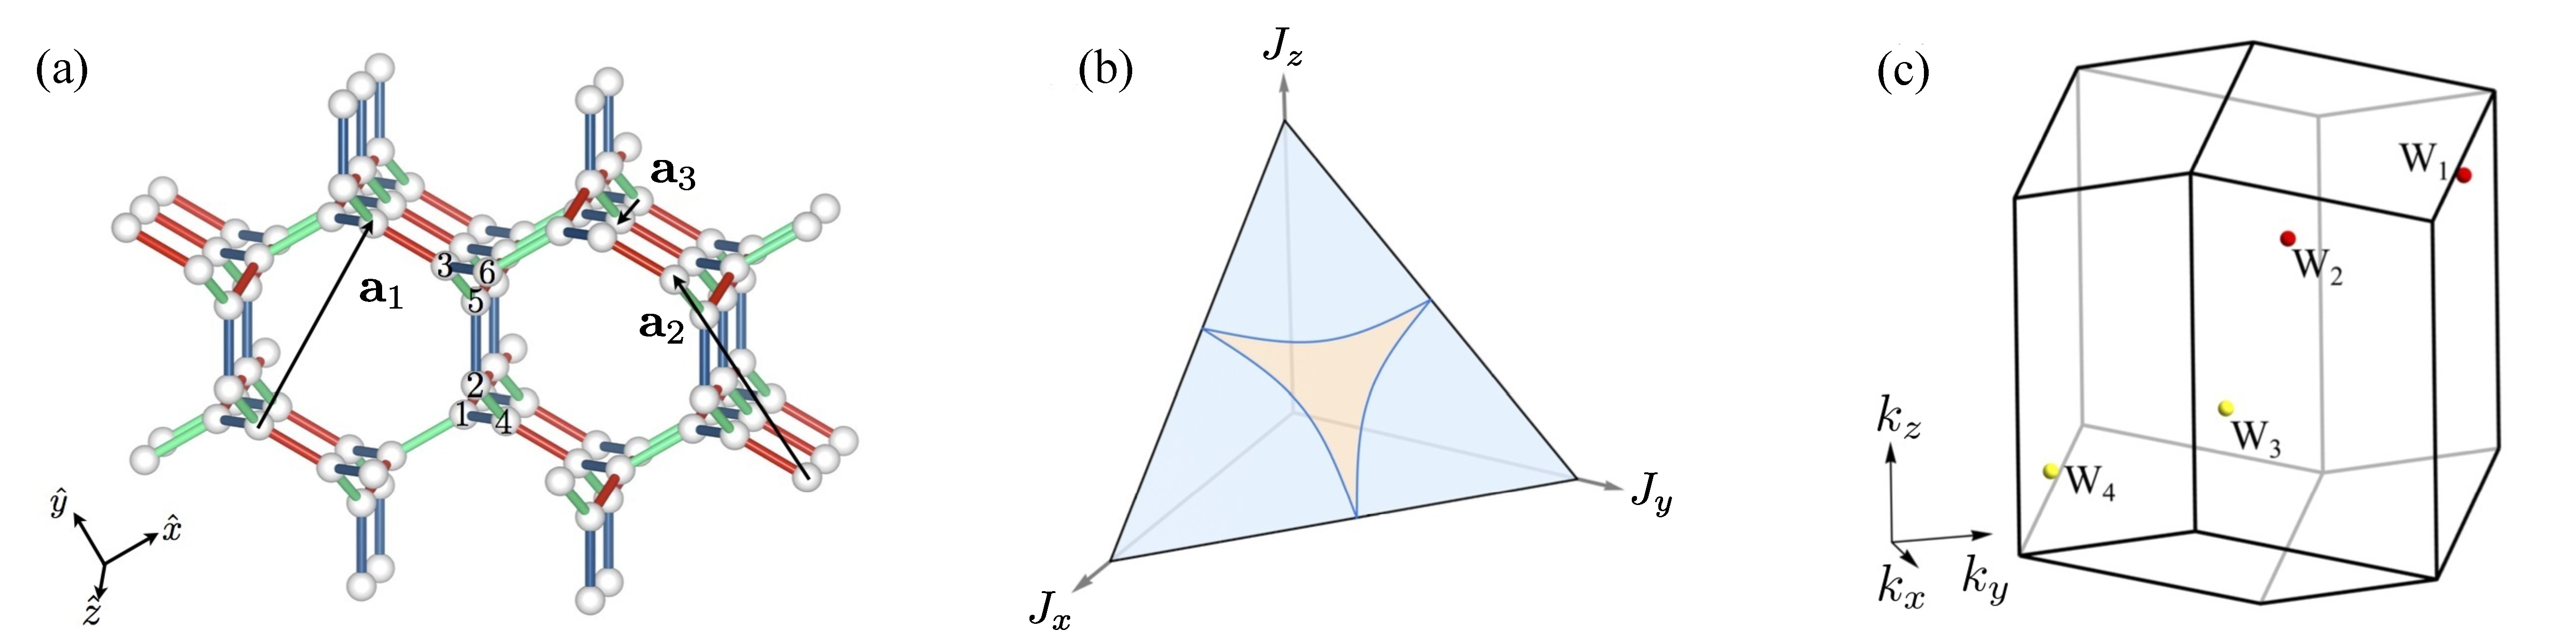
\includegraphics[width=\linewidth]{./chapter05/8_3bPanel.pdf}
	\caption{
		(a) Unit cell and translation vectors for the Kitaev model on lattice (8,3)b.
		(b) Ground state phase diagram for lattice (8,3)b.
		The regions orange shaded region corresponds to the gapless Weyl spin liquid phase.
		The blue shaded regions are gapped.
		(c) Visualization of the four Weyl nodes for isotropic exchange couplings.
		Weyl nodes of positive and negative chirality are denoted by red and yellow, respectively.
		Note that the Weyl nodes all lie on a $C_3$-invariant axis which does not pass through the origin due to its projective representation inducing a shift in momentum space.
	}
	\label{fig:chapter05_8_3bPanel}
\end{figure}
%


%
%
\subsubsection{Gauge structure}
%
%
Lattice (8,3)b possesses three loop operators of length 8 and one of length 12 per unit cell.
These four loop operators may be combined to form a closed volume leading to only \textit{three} independent loop operators per unit cell (see Appendix~\ref{appendix:ThreeDimensionalKitaevModels_8_3b} for details).
The canonical flux sector for lattice (8,3)b corresponds to $\pi$-flux through all elementary loops.
This results in all loop operators $\op{W}_p$ having eigenvalue +1.
Additionally, it has been checked numerically that the canonical flux sector is, indeed, the ground state flux sector.
The vison gap $\Delta \sim 0.16$ for lattice (8,3)b is the largest found for the lattices considered here (see Figure~\ref{fig:chapter05_VisonGaps} and Table~\ref{table:chapter05_VisonGaps}).
The vison gap has been computed by flipping the value of $u_{jk}$ for a single $z$-bond, resulting in the excitation of four loop operators (further details are given in Appendix~\ref{appendix:ThreeDimensionalKitaevModels_8_3b}).


%
%
\subsubsection{Projective symmetries}
%
%
Lattice (8,3)b is bipartite with different sublattices connected by the vectors $\br_0 = \ba_1$ and $\br'_0 = \ba_3$.
As a result, the projective representation of time-reversal is given by
%
\begin{equation}
	H(\bk) = G\dag_{\mathcal{T}}~H(-\bk + \bk_0) G_{\mathcal{T}},
\end{equation}
%
where $\bk_0 = (\bq_1 + \bq_3)/2$ and the associated gauge transformation matrix is given by
%
\begin{equation}
	G_{\mathcal{T}} =
		\begin{pmatrix}
			\id & 0 \\
			0	& -\id
		\end{pmatrix}.
\end{equation}
%
Furthermore, the lattice is inversion symmetric with projective representation
%
\begin{equation}
	H(\bk) = G\dag_{\mathcal{P}}~U_{\mathcal{P}}~H(-\bk)~U\dag_{\mathcal{P}}~G_{\mathcal{P}},
\end{equation}
%
where $U_{\mathcal{P}}$ is the matrix representation of the inversion operator acting on the unit cell indices, and the associated gauge transformation matrix $G_{\mathcal{P}}$ is identical to $G_{\mathcal{T}}$ for the gauge \textit{Ansatz} used here.
Note, however, that the gauge transformation $\op{G}_{\mathcal{P}}$ associated to the inversion operator does \textit{not} oscillate sign as a function of unit cell position $\br$ and, thus, yields a projective inversion operator that relates states at $\bk$ to states at $-\bk$.
The resulting energy relations are given by
%
\begin{equation}
	E_{\alpha}(\bk) = -E_{\beta}(-\bk) \qquad E_{\alpha}(\bk) = E_{\gamma}(-\bk + \bk_0) \qquad E_{\alpha}(\bk) = E_{\delta}(-\bk),
\end{equation}
%
due to particle-hole, time-reversal and inversion symmetry, respectively.
Due to the fact that the gauge transformation $\op{G}_{\mathcal{T}}$ relates states at momentum $\bk$ to states at momentum $\bk - \bk_0$, the momentum space Hamiltonian matrix has the form of a generic band Hamiltonian
%
\begin{equation}
	H(\bk) = 
		\begin{pmatrix}
			0			&			& A(\bk) 	\\
			& \ddots 	& 			\\
			A\dag(\bk)	&			& 0
		\end{pmatrix}
	\label{eq:chapter05_8_3bGenericHamiltonian}
\end{equation}
%
similar to lattice (8,3)a, however, with the additional property that it is inversion symmetric.


%
\subsubsection{Majorana band structure}
%
The presence of a trivially implemented projective inversion symmetry, \ie, with $\til{\bk}_0 = \bm{0}$, prohibits the formation of stable Fermi surfaces.
This can be seen by noting that the combination of particle-hole and inversion symmetries yields the relation $E_{\alpha}(\bk) = - E_{\beta}(\bk)$, preventing an isolated band from crossing the Fermi energy.
Furthermore, a doubly degenerate two-dimensional Fermi surface, while allowed by symmetry, is purely accidental and may be gapped by simply tuning the exchange couplings.

The spectrum may, however, contain the type of topological degeneracies discussed in Section~\ref{section:chapter05_8_3a}.
In this case, the degenerate bands $E_{\pm}(\bk)$ are described locally by
%
\begin{equation}
	E_{\pm}(\bk) \approx E_0(\bk^*) \pm \sum_i~b^i |k_i - k^*_i| \qquad {\rm where } \qquad b^i \in \mathbb{R}_{+}.
\end{equation}
%
Note that non-zero $E_0(\bk^*)$ may yield two-dimensional Fermi surfaces, but, as mentioned above, such Fermi surfaces are unstable.
In the case that $E_0(\bk^*) = 0$, however, these degeneracies remain pinned to zero-energy by the combination of inversion and particle-hole symmetries.

Such a degeneracy is described locally by the effective two-band Hamiltonian
%
\begin{equation}
	H_{\rm Weyl}(\bk) = \sum_{j=1}^{3}~ \bm{v}_j \cdot (\bk - \bk^*)~\tau^j,
	\label{eq:chapter05_WeylHamiltonian}
\end{equation}
%
where $\bk^*$ is the location of the degeneracy, the Fermi velocities $\bm{v}_j \in \mathbb{R}^3\backslash\{\bm{0}\}$ are linearly-independent, and $\tau^j$ are Pauli matrices acting on the degenerate bands.
This Hamiltonian may be recognized as the Weyl Hamiltonian (with anisotropic speed of light) of high-energy theory which describes massless, chiral fermions.
As such, these zero-energy degeneracies are referred to as \textit{Weyl nodes}.
Each Weyl node has a topological charge associated to its chirality which may be calculated as $\signum{[\bm{v}_1 \cdot (\bm{v}_2 \times \bm{v}_3)]}$.
More physically, Weyl nodes may be identified as monopoles of the Berry flux, where the charge of the monopole is equal to the chirality of the Weyl node.
%
\begin{figure}[tb]
	\centering
	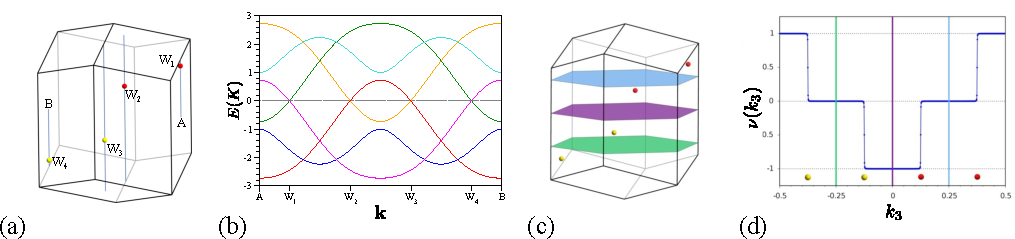
\includegraphics[width=\linewidth]{./chapter05/8_3bPanel2.pdf}
	\caption{
		(a) The Weyl nodes of lattice (8,3)b are located on the $C_3$-invariant axis, marked in blue.
		(b) Majorana dispersion plotted along the $C_3$-axis.
		(c) Brillouin zone with positions of the Weyl nodes and three example planes for which the Chern number may be calculated
		(d) Chern number $\nu(k_3)$ plotted as a function of $k_3$.
		The positions of the Weyl nodes and three example planes  ($k_3 = 0, \pm 1/4$) are indicated as a guide to the eye.
	}
	\label{fig:chapter05_8_3bPanel2}
\end{figure}
%

The form of Eq.~\eqref{eq:chapter05_WeylHamiltonian} implies that the particle-hole transformation inherent to the Kitaev spin liquids requires the presence of Weyl nodes of opposite chirality at opposite momenta $\bk^*$ and $-\bk^*$.
Similarly, the presence of inversion symmetry would imply the existence of Weyl nodes of opposite chirality at momenta $\bk^*$ and $-\bk^* + \til{\bk}_0$.
Furthermore, the presence of time-reversal symmetry would imply Weyl nodes of the \textit{same} chirality at momenta $\bk^*$ and $-\bk^* + \bk_0$.
Note that in a normal fermionic system, the presence of \textit{both} inversion and time-reversal symmetries does not allow for stable Weyl nodes, as the symmetries act to map Weyl nodes of opposite chirality onto one another.
However, the fact that the symmetries must be represented \textit{projectively} in the fermionic sector of the Kitaev spin liquid allows for the unique possibility of having a stable \textit{Weyl spin liquid} phase where both inversion and time-reversal symmetries are present.

Diagonalizing the concrete Kitaev Hamiltonian for lattice (8,3)b reveals an extended gapless Weyl spin liquid phase around the point of isotropic exchange couplings (see phase diagram in Figure~\ref{fig:chapter05_8_3bPanel}~(b)).
Due to the periodicity of the Brillouin zone, the overall Berry charge must vanish and, thus, Weyl nodes always appear in pairs of opposite chirality.
From the above discussion, it is clear that for lattice (8,3)b there must be at least four Weyl nodes due to the presence of particle-hole symmetry along with inversion symmetry (with $\til{\bk}_0 = 0$) and time-reversal symmetry.
For isotropic couplings, there are four Weyl nodes which all lie on a $C_3$-invariant axis (see Figure~\ref{fig:chapter05_8_3bPanel}~(c) or Figure~\ref{fig:chapter05_8_3bPanel2}~(a) and (b)).
Two Weyl nodes of positive charge are located at $W_1 = (5/8)\bq_1 + (3/4)\bq_2 + (3/8)\bq_3$ and $W_2 = -W_2 + \bk_0$, whereas there are two negatively charged Weyl nodes located at $W_3 = -W_2$ and $W_4 = -W_1$.

The charge of a Weyl node can be measured by computing the Chern number on an arbitrary surface which encloses it.
Due to the periodicity of the Brillouin zone, such a closed surface may be deformed into a pair of planes lying on either side of the Weyl node (refer to Figure~\ref{fig:chapter05_8_3bPanel2}~(c)).
Reversing the orientation of \textit{one} of the planes, such that both planes now have the same orientation, reverses the Chern number of that plane.
The result is that the Chern number of the original closed surface, \ie, the chirality of the Weyl node, is given by the \textit{difference} in Chern numbers between the two planes.
The Chern number for the Kitaev Hamiltonian on lattice (8,3)b with isotropic couplings is plotted as a function of $k_3 = \bk \cdot \bq_3 / 2\pi$ in Figure~\ref{fig:chapter05_8_3bPanel2}~(d), \ie, each plane has a fixed value of $k_3$.
One may see that at $k_3$-values corresponding to a plane containing a Weyl node, the Chern number jumps by the respective charge of that Weyl node.

Figure~\ref{fig:chapter05_8_3bWeyl1}~(a) shows the evolution of the Weyl nodes in the 3D Brillouin zone as the exchange couplings are varied for $0 \leq J_z \lesssim 0.43$ with $J_x = J_y = (1 - J_z)/2$.
The trajectory of negatively charged Weyl nodes changes colors from yellow to green as $J_z$ is increased, whereas the trajectory of positively charged Weyl nodes changes from red to green.
As $J_z$ is increased, Weyl nodes of opposite chirality move towards each other, ultimately meeting and mutually annihilating at the $\Gamma$-point and at $\bk_0$ for $J_z \approx 0.43$.
For decreasing $J_z$, the Weyl nodes similarly move through the Brillouin zone, however, rather than meeting and mutually annihilating at isolated momenta, the velocity vectors of the isolated Weyl nodes vanish, collapsing the bulk gap.
Note that, away from the isotropic point the $C_3$-symmetry is broken and, thus, the Weyl nodes are free to leave the $C_3$-invariant axis.
%
\begin{figure}[tb]
	\centering
	
\includegraphics[width=\linewidth]{./chapter05/8_3bWeyl1.pdf}
	\caption{
		(a) Evolution of Weyl nodes of lattice (8,3)b for varied coupling constants $0 \leq J_z \lesssim 0.43$ with $J_x = J_y = (1 - J_z)/2$.
		(b) Corresponding Fermi arc evolution.
		(c) Visualization of the surface Brillouin zone for the 001-surface.
	}
	\label{fig:chapter05_8_3bWeyl1}
\end{figure}
%

Figure~\ref{fig:chapter05_8_3bWeyl1}~(b) shows the associated Fermi arc surface states for the 001-surface Brillouin zone of a slab geometry.
The surface Brillouin zone is visualized in Figure~\ref{fig:chapter05_8_3bWeyl1}~(c).
Fermi arcs are exact zero-energy surface states which connect Weyl nodes of opposite chirality (more accurately, their projections to the surface Brillouin zone).
The Fermi arcs inherit a topological protection from their associated Weyl nodes -- as long as the Weyl nodes are left intact, no perturbation can gap their surface states.
As the Weyl nodes wander through the bulk Brillouin zone, the Fermi arcs are seen to deform, ultimately shrinking to nothing as the Weyl nodes meet and annihilate for $J_z \approx 0.43$.

Breaking time-reversal symmetry by applying an external magnetic field also causes the Weyl nodes to wander around the Brillouin zone as seen in Figure~\ref{fig:chapter05_8_3bWeyl2}~(a) for $0 \leq \kappa \leq 0.25$.
At $\kappa \approx 0.2$, two Weyl nodes of opposite chirality meet and mutually annihilate at a high-symmetry point in the Brillouin zone.
Note that, since application of a magnetic field in the 111-direction does not break $C_3$-symmetry, the Weyl nodes are pinned to the $C_3$-invariant axis.
In Figure~\ref{fig:chapter05_8_3bWeyl2}~(b) are pictured the corresponding Fermi arcs in the 001-surface Brillouin zone.
As $\kappa$ is tuned from 0 to 0.2, the Fermi arcs become increasingly warped as two Weyl nodes of opposite chirality move towards each other.
As $\kappa$ is increased further, the two Fermi arcs meet at a high-symmetry point, becoming a single Fermi arc.
For still larger values of $\kappa$, even more Weyl nodes begin to appear in charge-neutral pairs while other pairs mutually annihilate.
%
\begin{figure}[tb]
	\centering
	
\includegraphics[width=\linewidth]{./chapter05/8_3bWeyl2.pdf}
	\caption{
		(a) Evolution of Weyl nodes of lattice (8,3)b in the presence of a magnetic field of varied strength $0 \leq \kappa \leq 0.25$.
		(b) Corresponding Fermi arc evolution.
		(c) Visualization of the surface Brillouin zone for the 001-surface.
	}
	\label{fig:chapter05_8_3bWeyl2}
\end{figure}
%


%
%
% LATTICE (8,3)C %%%%%%%%%%%%%%%%%%%%%%%%%%%%%%%%%%%%%%%%%%%%%%%%%%%%%%%%%%%%%%%%%%%%%%%
\subsection{Lattice (8,3)c}
\label{section:chapter05_8_3c}
%%%%%%%%%%%%%%%%%%%%%%%%%%%%%%%%%%%%%%%%%%%%%%%%%%%%%%%%%%%%%%%%%%%%%%%%%%%%%%%%%%%%%%%%
%
%
\subsubsection{Lattice information}
%
%
Lattice (8,3)c can be viewed as parallel zigzag chains which run along the $z$-direction and which are coupled by vertices lying in the $x-y$ plane.
Formally, lattice (8,3)c is specified by the hexagonal space group $P6_{3}/mmc$ (No. 194) with $c/a = 2/5$ and Wyckoff positions for the unit cell are $2(c)$ and $6(h)$ with $x=7/15$.
The concrete choice of eight site unit cell used in this work is given by the site positions
%
\begin{equation}
	\begin{matrix*}[l]
		\br_1 = \left(-\frac{1}{5}, \frac{4}{5\sqrt{3}}, \frac{1}{10}\right) &
		\br_2 = \left(0, \frac{7}{5\sqrt{3}}, \frac{1}{10}\right) &
		\br_3 = \left(\frac{1}{5}, \frac{4}{5\sqrt{3}}, \frac{1}{10}\right) \\
		&\\
		\br_4 = \left(\frac{1}{2}, \frac{1}{2\sqrt{3}}, \frac{3}{10}\right) &
		\br_5 = \left(0, \frac{1}{\sqrt{3}}, \frac{1}{10}\right) &
		\br_6 = \left(\frac{3}{10}, \frac{7}{10\sqrt{3}}, \frac{3}{10}\right) \\
		&\\
		\br_7 = \left(\frac{1}{2}, \frac{1}{10\sqrt{3}}, \frac{3}{10}\right) &
		\br_8 = \left(\frac{7}{10}, \frac{7}{10\sqrt{3}}, \frac{3}{10}\right).
	\end{matrix*}
\end{equation}
%
The lattice vectors are chosen to be
%
\begin{equation}
	\begin{matrix*}[l]
		\ba_1 = \left(1, 0, 0\right) \qquad
		\ba_2 = \left(-\frac{1}{2}, \frac{\sqrt{3}}{2}, 0\right) \qquad
		\ba_3 = \left(0, 0, \frac{2}{5}\right)
	\end{matrix*}
\end{equation}
%
with the corresponding reciprocal lattice vectors
%

%
\begin{equation}
	\begin{matrix*}[l]
		\bq_1 = \left(2\pi, \frac{2\pi}{\sqrt{3}}, 0\right) \qquad
		\bq_2 = \left(0, \frac{4\pi}{\sqrt{3}}, 0\right) \qquad
		\bq_3 = \left(0, 0, 5\pi\right).
	\end{matrix*}
\end{equation}
%

The unit cell and translation vectors are illustrated in Figure~\ref{fig:chapter05_8_3cPanel}~(a).
The bonds in the figure are colored red, green and blue to indicate the assignment of $x$-, $y$- and $z$-type bonds, respectively.
When choosing the assignment of bonds for this lattice, one finds that for each of the chains there are two inequivalent choices.
The assignment of bonds used here is chosen to respect as many of the lattice symmetries as possible. 
More specifically, there are two distinct sets of $x$-, $y$- and $z$-bonds, namely those forming the zigzag chains along the z-direction and those lying in the $x-y$ plane.
The set of all $x$-, $y$- and $z$-bonds are related to each other by a sixfold screw axis.
The symmetry between $x$-, $y$- and $z$-bonds is reflected in the phase diagram shown in Figure~\ref{fig:chapter05_8_3cPanel}~(b).
%
\begin{figure}[tb]
	\centering
	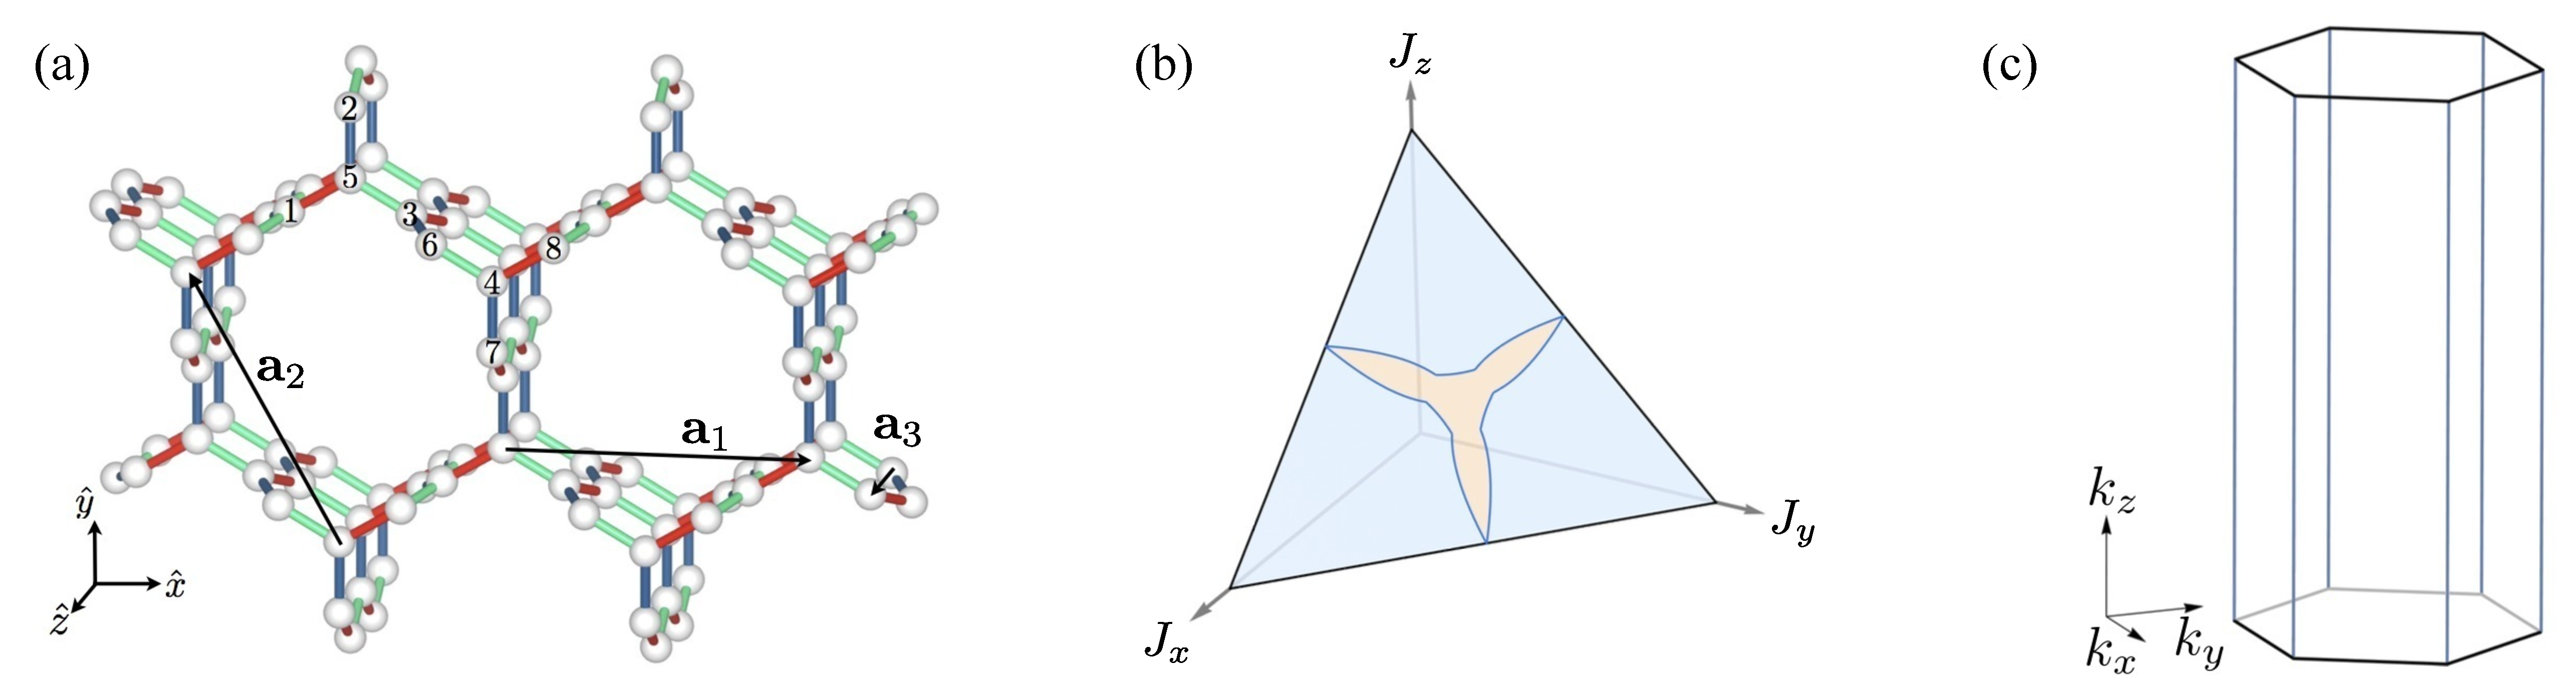
\includegraphics[width=\linewidth]{./chapter05/8_3cPanel.pdf}
	\caption{
		(a) Unit cell and translation vectors for the Kitaev model on lattice (8,3)c.
		(b) Phase diagram for lattice (8,3)c.
		The orange shaded regions correspond to a gapless phase with line nodes.
		The blue shaded regions are gapped.
		(c) The line nodes (marked in blue) are located precisely at the edges of the Brillouin zone for isotropic exchange couplings.
	}
	\label{fig:chapter05_8_3cPanel}
\end{figure}
%


%
%
\subsubsection{Gauge structure}
%
%
Lattice (8,3)c possesses six loop operators of length 8 and one of length 18 per unit cell.
These seven loop operators may be combined to form three closed volumes leading to only \textit{four} independent loop operators per unit cell (see Appendix~\ref{appendix:ThreeDimensionalKitaevModels_8_3c} for details).
The canonical flux sector for lattice (8,3)c corresponds to $\pi$-flux through all loops of length 8 and $0$-flux through all loops of length 18.

It turns out, however, that it is not possible to achieve the canonical flux sector for lattice (8,3)c.
As it takes three loops of length 8 to form a closed volume which is constrained to have vanishing total flux, one may assign $\pi$-flux either to only two of the loops or to none of the loops.
Lieb's theorem indicates that the system would prefer to thread $\pi$-flux through as many plaquettes as possible and, thus, the former option leads to lower energy.
Unfortunately, it is not \textit{a priori} clear which of the plaquettes should be assigned $0$-flux.

For highly anisotropic couplings, \eg, $J_z \gg J_x = J_y$, there exists a unique ground state flux configuration corresponding to a threading of $\pi$-flux through the loops which contain three $z$-bonds and $0$-flux through the two remaining loops which contain only two $z$-bonds, a result which is derived in Appendix~\ref{appendix:LoopModels_8_3c}.
This perturbative result was later confirmed by a subsequent quantum Monte Carlo study~\cite{EschmannPRL2019} of the Kitaev model on lattice (8,3)c.
Additionally, this study suggests that at the isotropic point, there is a sub-extensive degeneracy of ground states with columnar flux order.
Away from the isotropic point, where $C_3$ symmetry is broken explicitly, however, the system uniquely selects one of these ground states.

The work presented in this chapter, however, does not tackle the problem of finding the actual ground state flux configuration of the system.
Instead, the flux sector corresponding to all plaquettes having $0$-flux is used to illustrate the ideas of the classification scheme.
This flux sector is the only one which respects all of the lattice symmetries, but is not frustrated.
Such a flux sector can always be stabilized as the ground state by adding terms to the Hamiltonian which penalize $\pi$-flux through plaquettes, similar to what was done in Reference~\cite{LaiPRB2011} for the Kitaev model on the two-dimensional square-octagon lattice.
Note that the results reported below are, indeed, qualitatively correct also for the true ground state spin liquid on lattice (8,3)c.
The vison gap for lattice (8,3)c is not reported here as calculations were not done in the ground state sector, however, it is worth noting that an elementary vison excitation results in the excitation of four loop operators (further details are given in Appendix~\ref{appendix:ThreeDimensionalKitaevModels_8_3c}).


%
%
\subsubsection{Projective symmetries}
%
%
Lattice (8,3)c is bipartite with sublattices having the same translation symmetry as the elementary unit cell.
The resulting projective representation of time-reversal is given by
%
\begin{equation}
	H(\bk) = G\dag_{\mathcal{T}}~H(-\bk)~G_{\mathcal{T}},
\end{equation}
%
where the associated gauge transformation matrix is given by
%
\begin{equation}
	G_{\mathcal{T}} =
		\begin{pmatrix}
			\id & 0 \\
			0	& -\id
		\end{pmatrix}.
\end{equation}
%
Furthermore, the lattice is inversion symmetric with projective representation
%
\begin{equation}
	H(\bk) = G\dag_{\mathcal{P}}~U_{\mathcal{P}}~H(-\bk)~U\dag_{\mathcal{P}}~G_{\mathcal{P}},
\end{equation}
%
where $U_{\mathcal{P}}$ is the matrix representation of the inversion operator acting on the unit cell, and the associated gauge transformation matrix $G_{\mathcal{P}}$ is identical to $G_{\mathcal{T}}$ for the gauge \textit{Ansatz} used here.
The resulting energy relations are given by
%
\begin{equation}
	E_{\alpha}(\bk) = -E_{\beta}(-\bk) \qquad {\rm and } \qquad E_{\alpha}(\bk) = E_{\gamma}(-\bk),
\end{equation}
%
where the first relation is due to particle-hole symmetry and the second is enforced individually by both time-reversal and inversion symmetry.
Due to the fact that the gauge transformation $\op{G}_{\mathcal{T}}$ is constant as a function of unit cell position,
the momentum space Hamiltonian matrix has the block off-diagonal form
%
\begin{equation}
	H(\bk) =
		\begin{pmatrix}
			0			& A(\bk) \\
			A\dag(\bk)	& 0
		\end{pmatrix}.
		\label{eq:chapter05_8_3cGenericHamiltonian}
\end{equation}
%


%
%
\subsubsection{Majorana band structure}
%
%
As was the case for lattice (8,3)b, a trivially implemented projective inversion symmetry prevents the formation of stable Fermi surfaces.
Unlike lattice (8,3)b, however, the projective time-reversal operator is also implemented trivially, yielding a block off-diagonal Hamiltonian matrix as in Eq.~\eqref{eq:chapter05_8_3cGenericHamiltonian}.
Zero modes at a given momentum correspond to vanishing of the determinant of $H(\bk)$, which, in this case, means the simultaneous vanishing of $\Re{(\det{A(\bk)})}$ and $\Im{(\det{A(\bk)})}$.
In three-dimensions, solutions to the above correspond to a one-dimensional manifold of $\bk$-points.
The conclusion is that for the Kitaev model defined on lattice (8,3)c, the only stable zero-energy manifolds are \textit{nodal lines}.

In fact, such nodal lines are protected by the presence of time-reversal symmetry and may be characterized by an integer invariant~\cite{BurkovPRB2011,ZhaoPRL2013,MatsuuraNJP2013}
%
\begin{equation}
	\nu = -\frac{1}{2\pi} \Im{\oint_S}~dt~\trace{[\partial_t \log A(\bk)]},
\end{equation}
%
where $S$ is a closed path in momentum space parameterized by $t$, and $\nu$ is seen to be the winding number of the map $\bk \in S \mapsto A(\bk)$.
For loops $S$ which are pierced by the nodal line, this winding number is non-zero.
As this integer winding number cannot be changed continuously, it represents an obstruction to gapping out the nodal line.
Thus, without breaking time-reversal symmetry, this can only be done by shrinking the nodal line to a point.
If time-reversal symmetry is broken, however, the winding number is no longer well-defined and such a nodal line becomes unstable.

Diagonalizing the concrete Kitaev Hamiltonian for lattice (8,3)c reveals an extended gapless phase around the point of isotropic exchange couplings (see Figure~\ref{fig:chapter05_8_3cPanel}~(b)), where the zero modes correspond to nodal lines located at $(\pm\frac{4\pi}{3}, 0, k_z)$ as pictured in Figure~\ref{fig:chapter05_8_3cPanel}~(c).
Also visible in the Figure is a surface of gapless modes at the top (bottom) of the Brillouin zone.
As discussed above, this surface cannot be stable and, in fact, gaps out as soon as the couplings are tuned away from the isotropic point.

As mentioned above, the nodal line is protected by the presence of time-reversal symmetry.
Introducing an infinitesimal external magnetic field immediately gaps the nodal line almost entirely.
However, adding a magnetic field term to the model does not break the inversion symmetry of lattice (8,3)c.
As a result, for fixed $\bk$, the Hamiltonian is of the same form as that discussed for lattice (8,3)b, where time-reversal symmetry was present, albeit with a shift in momentum space.
As a result, the nodal line is gapped with the exception of six isolated points corresponding to stable Weyl nodes.
A similar situation was studied in Reference~\cite{HermannsPRL2015} for lattice (10,3)b and is discussed in Section~\ref{section:chapter05_10_3b}.
%
\begin{figure}[tb]
	\centering
	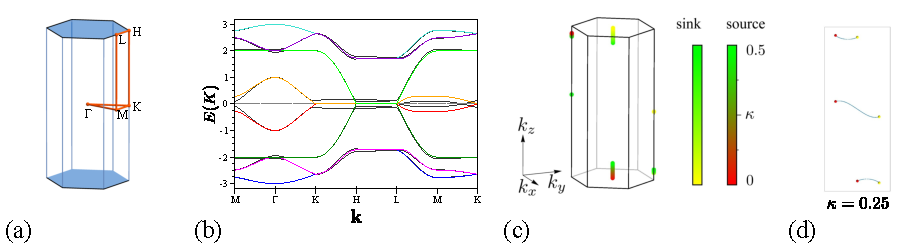
\includegraphics[width=\linewidth]{./chapter05/8_3cPanel2.pdf}
	\caption{
		(a) Brillouin zone of lattice (8,3)c with high-symmetry points.
		The nodal lines and surfaces are marked in blue.
		(b) Majorana dispersion plotted along the high-symmetry paths.
		(c) Evolution of the Weyl nodes in the presence of a magnetic field of varying strength $0 \leq \kappa \leq 0.5$.
		(d) Corresponding Fermi arcs for $\kappa = 0.25$.
	}
	\label{fig:chapter05_8_3cPanel2}
\end{figure}
%

The evolution of these Weyl nodes is pictured in Figure~\ref{fig:chapter05_8_3cPanel2}~(c) for varying magnetic field strengths corresponding to $0 \leq \kappa \leq 0.5$.
For this range of $\kappa$, the Weyl nodes move very little along high-symmetry lines of the Brillouin zone.
However, for larger values of $\kappa$, many Weyl nodes appear in charge-neutral pairs while other pairs mutually annihilate.
In Figure~\ref{fig:chapter05_8_3cPanel2}~(d) are pictured the corresponding Fermi arc surface states in the 100-surface Brillouin zone for $\kappa = 0.25$.


%
%
% LATTICE (8,3)N %%%%%%%%%%%%%%%%%%%%%%%%%%%%%%%%%%%%%%%%%%%%%%%%%%%%%%%%%%%%%%%%%%%%%%%
\subsection{Lattice (8,3)n}
\label{section:chapter05_8_3n}
%%%%%%%%%%%%%%%%%%%%%%%%%%%%%%%%%%%%%%%%%%%%%%%%%%%%%%%%%%%%%%%%%%%%%%%%%%%%%%%%%%%%%%%%
%
%
\subsubsection{Lattice information}
%
%
Lattice (8,3)n can be viewed as a three-dimensional generalization of the square-octagon lattice, where layers of square-octagon lattices are coupled via mid-bond sites.
Formally, lattice (8,3)n is specified by the tetragonal space group $I4/mmm$ (No. 139) with $c/a = \frac{4}{2\sqrt{3} + \sqrt{2}}$ and Wyckoff positions for the unit cell are $16(k)$ and $16(n)$ with $x = \frac{\sqrt{3} + \sqrt{2}}{2(2\sqrt{3} + \sqrt{2})}$ and $z=1/8$.
The concretely choice of unit cell used in this work has 16 sites.
In order to simplify notation, the following basis is defined:
%
\begin{equation}
	\begin{matrix*}[l]
		\ba = \left(1, 0, 0\right) \qquad
		\bb = \left(0, 1, 0\right) \qquad
		\bc = \left(0, 0, \frac{4}{2\sqrt{3} + \sqrt{2}}\right).
	\end{matrix*}
\end{equation}
%
In the basis $(\ba, \bb, \bc)$, the positions of the sites are given by\pagebreak
%
\begin{equation}
	\begin{matrix*}[l]
		\br_{1} = \left(\frac{1}{2} + x, x, \frac{1}{4} \right) &
		\br_{2} = \left(\frac{3}{2} - x, x, \frac{1}{4} \right) &
		\br_{3} = \left(\frac{3}{2} - x, 1 - x, \frac{1}{4} \right) \\
		&\\
		\br_{4} = \left(\frac{1}{2} + x, 1 - x, \frac{1}{4} \right) &
		\br_{5} = \left(1, x, -z \right) &
		\br_{6} = \left(\frac{3}{2} - x, \frac{1}{2}, -\frac{1}{2} + z \right) \\
		&\\
		\br_{7} = \left(1, 1 - x, -z \right) &
		\br_{8} = \left(\frac{1}{2} + x, \frac{1}{2}, -\frac{1}{2} + z \right) &
		\br_{9} = \left(\frac{1}{2} + x, \frac{1}{2}, \frac{1}{2} - z \right) \\
		&\\
		\br_{10} = \left(1, x, z \right) &
		\br_{11} = \left(\frac{3}{2} - x, \frac{1}{2}, \frac{1}{2} - z \right) &
		\br_{12} = \left(1, 1-x, z \right) \\
		&\\
		\br_{13} = \left(\frac{1}{2} + x, x, -\frac{1}{4} \right) &
		\br_{14} = \left(\frac{3}{2} - x, x, -\frac{1}{4} \right) &
		\br_{15} = \left(\frac{3}{2} -x, 1 - x, -\frac{1}{4} \right) \\
		&\\
		\br_{16} = \left(\frac{1}{2} + x, 1 - x, -\frac{1}{4} \right),
	\end{matrix*}
\end{equation}
%
where $x = \frac{\sqrt{3} + \sqrt{2}}{2(2\sqrt{3} + \sqrt{2})}$ and $z=1/8$.
The lattice vectors are chosen to be
%
\begin{equation}
	\begin{matrix*}[l]
		\ba_1 = \ba \qquad
		\ba_2 = \bb \qquad
		\ba_3 = \frac{1}{2}(\ba + \bb + \bc)
	\end{matrix*}
\end{equation}
%
with the corresponding reciprocal lattice vectors (passing back to the standard orthonormal basis)
%
\begin{equation}
	\begin{matrix*}[l]
		\bq_1 = \left(2\pi, 0, -\sqrt{\frac{7}{2} + \sqrt{6}}\pi\right) &
		\bq_2 = \left(0, 2\pi, -\sqrt{\frac{7}{2} + \sqrt{6}}\pi\right) \\
		&\\
		\bq_3 = \left(0, 0, 2\sqrt{\frac{7}{2} + \sqrt{6}}\pi\right). &
	\end{matrix*}
\end{equation}
%

The unit cell and translation vectors are illustrated in Figure~\ref{fig:chapter05_8_3nPanel}~(a).
The bonds in the figure are colored red, green and blue to indicate the assignment of $x$-, $y$- and $z$-type bonds, respectively.
This assignment of bonds is chosen to be compatible with the $C_4$ and inversion symmetries of the lattice and is unique up to an overall permutation of the bond types.
All $x$- and $y$-bonds are related by a combination of inversion, $C_4$ and mirror symmetries.
The $z$-bonds come in two distinct sets, namely, those which lie in the $x-y$ plane and connect nearest neighbor "squares" and those that lie along the $z$-direction and connect neighboring "square-octagon" planes.
All $z$-bonds contained within a given set are related to each other by $C_4$ symmetry.
However, $z$-bonds are not related to any other type of bond via lattice symmetries.
The symmetry between $x$- and $y$-bonds is reflected in the ground state phase diagram shown in Figure~\ref{fig:chapter05_8_3nPanel}~(b).
%
\begin{figure}[tb]
	\centering
	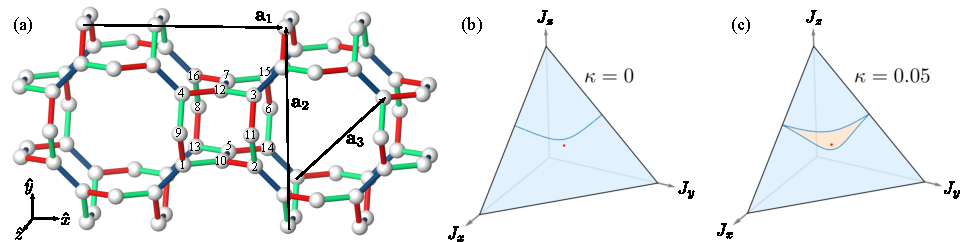
\includegraphics[width=\linewidth]{./chapter05/8_3nPanel.pdf}
	\caption{
		(a) Unit cell and translation vectors for the Kitaev model on lattice (8,3)n.
		(b) Ground state phase diagram for lattice (8,3)n.
		The Kitaev model on lattice (8,3)n has no gapless phase.
		The blue line indicates the phase transition between two distinct gapped phases.
		The isotropic point is denoted by a red dot.
		(c) Ground state phase diagram for $\kappa = 0.05$.
		For finite $\kappa$, the Dirac nodes split into pairs of oppositely charged Weyl nodes and the phase transition line evolves to a Weyl spin liquid phase, denoted by the orange shaded region.
	}
	\label{fig:chapter05_8_3nPanel}
\end{figure}
%


%
%
\subsubsection{Gauge structure}
%
%
Lattice (8,3)n possesses six loop operators of length 8, four of length 10, and two of length 12 per unit cell.
These twelve loop operators may be combined to form four closed volumes leading to only \textit{eight} independent loop operators per unit cell (see Appendix~\ref{appendix:ThreeDimensionalKitaevModels_8_3n} for details).
The canonical flux sector for lattice (8,3)n corresponds to $\pi$-flux through all loops of length 8 or 12 and $0$-flux through all loops of length 10.
This results in all loop operators $\op{W}_p$ having eigenvalue $+1$.
Additionally, it has been checked numerically that the canonical flux sector is, indeed, the ground state flux sector.
The vison gap for lattice (8,3)n shown in Figure~\ref{fig:chapter05_VisonGaps}~and Table~\ref{table:chapter05_VisonGaps}~has been computed by flipping the value of $u_{jk}$ for a single $z$-bond, resulting in the excitation of four loop operators (further details are given in Appendix~\ref{appendix:ThreeDimensionalKitaevModels_8_3n}).


%
\subsubsection{Projective symmetries}
%
%
Lattice (8,3)n is bipartite with sublattices having the same translation symmetry as the elementary unit cell.
The resulting projective representation of time-reversal is given by
%
\begin{equation}
	H(\bk) = G\dag_{\mathcal{T}}~H(-\bk)~G_{\mathcal{T}},
\end{equation}
%
where the associated gauge transformation matrix is given by
%
\begin{equation}
	G_{\mathcal{T}} =
		\begin{pmatrix}
			\id & 0 \\
			0	& -\id
		\end{pmatrix}.
\end{equation}
%
Furthermore, the lattice is inversion symmetric with projective representation
%
\begin{equation}
	H(\bk) = G\dag_{\mathcal{P}}~U_{\mathcal{P}}~H(-\bk + \til{\bk}_0)~U\dag_{\mathcal{P}}~G_{\mathcal{P}},
\end{equation}
%
where $\til{\bk}_0 = \bq_3/2$, $U_{\mathcal{P}}$ is the matrix representation of the inversion operator acting on the unit cell, and the associated gauge transformation matrix $G_{\mathcal{P}}$ is identical to $G_{\mathcal{T}}$  for the gauge \textit{Ansatz} used here.
The non-vanishing value of $\til{\bk}_0$ is due to the fact that, for a translationally invariant gauge \textit{Ansatz}, the gauge transformation $\op{G}_{\mathcal{P}}$ associated to the inversion operator oscillates sign as a function of unit cell position $\br$.
The resulting energy relations are given by
%
\begin{equation}
	E_{\alpha}(\bk) = -E_{\beta}(-\bk) \qquad E_{\alpha}(\bk) = E_{\gamma}(-\bk) \qquad E_{\alpha}(\bk) = E_{\delta}(-\bk + \til{\bk}_0),
\end{equation}
%
due to particle-hole, time-reversal and inversion symmetry, respectively.
Due to the fact that the gauge transformation $\op{G}_{\mathcal{T}}$ is constant as a function of unit cell position, the momentum space Hamiltonian matrix has the block off-diagonal form
%
\begin{equation}
	H(\bk) =
		\begin{pmatrix}
			0			& A(\bk) \\
			A\dag(\bk)	& 0
		\end{pmatrix}.
\end{equation}
%


%
%
\subsubsection{Majorana band structure}
%
%
As discussed in the context of lattice (8,3)c, due to the trivial implementation of the projective time-reversal operator, \ie, with $\bk_0 = 0$, the only stable nodal manifolds for lattice (8,3)n could be nodal lines.
In fact, what one finds upon diagonalization of the concrete Kitaev Hamiltonian, is that lattice (8,3)n turns out to be the only lattice considered in this work which does \textit{not} exhibit a gapless phase (see Figure~\ref{fig:chapter05_8_3nPanel}~(b) for the ground state phase diagram and Figure~\ref{fig:chapter05_8_3nPanel2}~(b) for the dispersion at the isotropic point).
Instead, there are two \textit{gapped} phases separated by a line of phase transitions for which the dispersion exhibits three-dimensional Dirac nodes of two doubly degenerate bands (see Figure~\ref{fig:chapter05_8_3nPanel2}~(c) and (d)).

One way of thinking of these three-dimensional Dirac nodes is as a combination of two oppositely charged Weyl nodes.
One way to split these Weyl nodes is by breaking time-reversal symmetry.
Indeed, introducing a magnet field splits the Dirac nodes into oppositely charged Weyl nodes as illustrated in Figure~\ref{fig:chapter05_8_3nPanel2}~(d).
As a result, this line of phase transitions becomes an extended gapless phase (see Figure~\ref{fig:chapter05_8_3nPanel}~(c)).
For small values of $\kappa$, this gapless phase is a Weyl spin liquid.
However, with time-reversal symmetry broken and projective inversion symmetry offering no protection, the Weyl nodes are not pinned to zero energy as is the case for lattices (8,3)b and (8,3)c above.
In fact, for sufficiently large values of $\kappa$, the degeneracies move away from zero energy, resulting in topologically protected Fermi surfaces as seen for lattice (8,3)a.
Note that the Fermi surfaces here are related by the perfect nesting vector $\til{\bk}_0$ due to the presence of inversion symmetry.
%
\begin{figure}[tb]
	\centering
	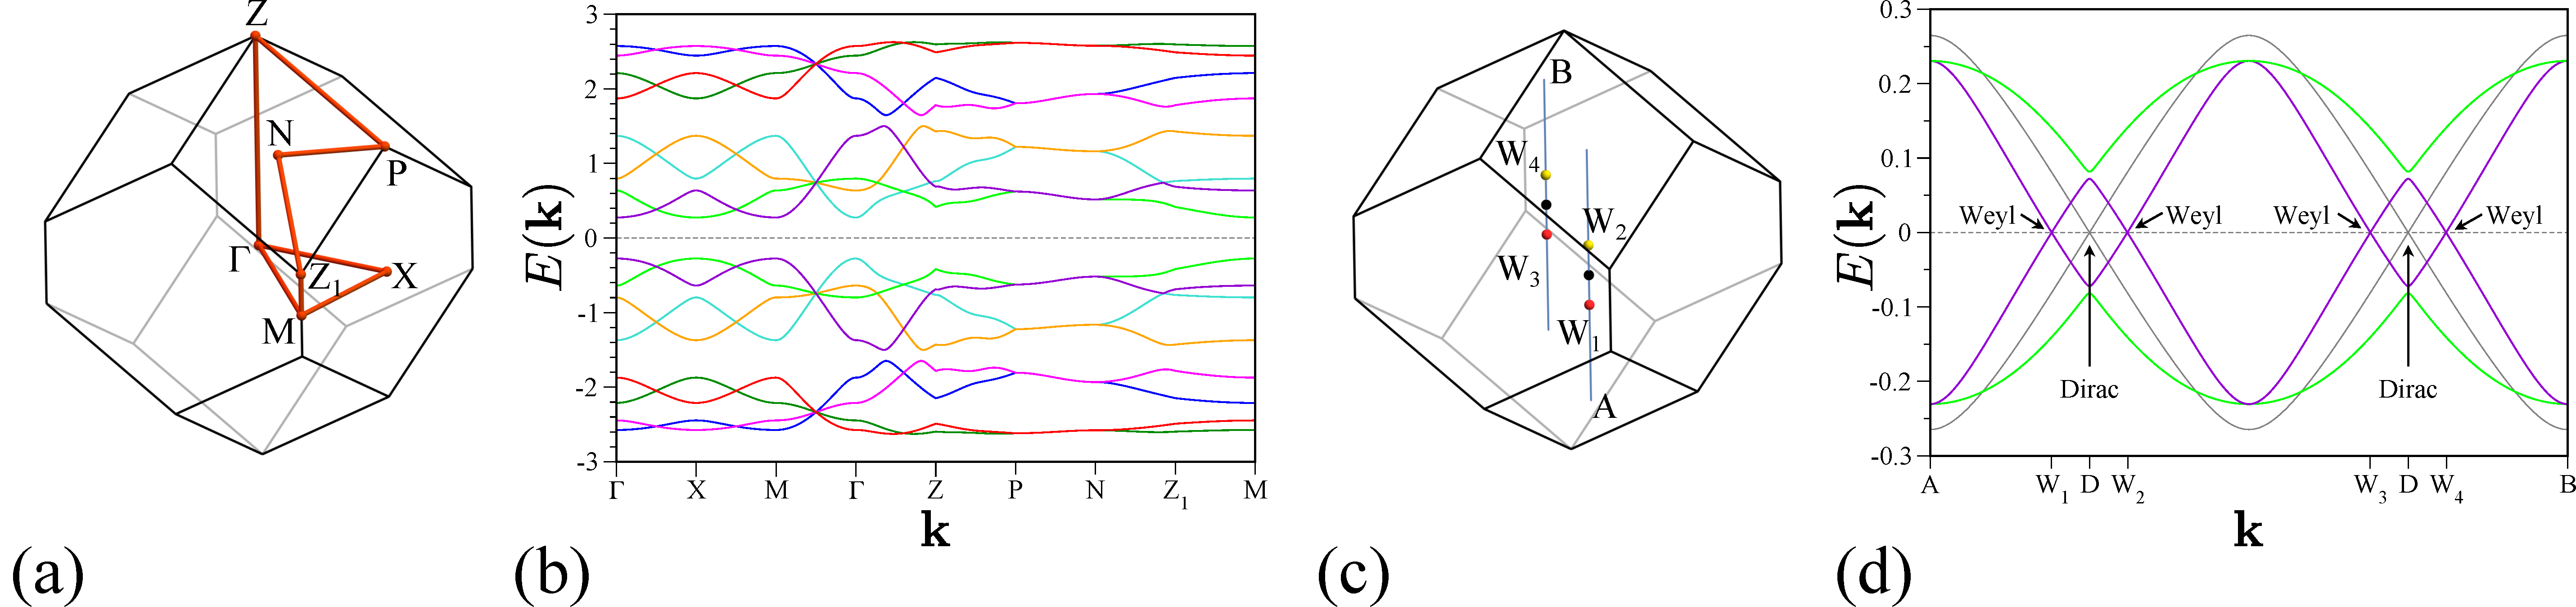
\includegraphics[width=\linewidth]{./chapter05/8_3nPanel2.pdf}
	\caption{
		(a) Brillouin zone of lattice (8,3)n with high-symmetry points.
		(b) Majorana dispersion plotted along a high-symmetry path.
		(c) Brillouin zone a path cutting through the Dirac/Weyl nodes.
		(d) Dispersion along the path in shown in (c).
		Gray lines correspond to $\kappa = 0$ while green lines correspond to $\kappa = 0.05$.
	}
	\label{fig:chapter05_8_3nPanel2}
\end{figure}
%


%
%
% LATTICE (9,3)A %%%%%%%%%%%%%%%%%%%%%%%%%%%%%%%%%%%%%%%%%%%%%%%%%%%%%%%%%%%%%%%%%%%%%%%
\subsection{Lattice (9,3)a}
\label{section:chapter05_9_3a}
%%%%%%%%%%%%%%%%%%%%%%%%%%%%%%%%%%%%%%%%%%%%%%%%%%%%%%%%%%%%%%%%%%%%%%%%%%%%%%%%%%%%%%%%
%
%
\subsubsection{Lattice information}
%
%
Lattice (9,3)a (subsequently referred to in the literature as the hypernonagon lattice~\cite{YasuyukiPRB2017,KatoPB2018,MasahikoPRL2018}) is the only non-bipartite lattice considered in this work.
Formally, lattice (8,3)a is specified by the trigonal space group $R\bar{3}m$ (No. 166) with $c/a = \frac{\sqrt{6(4 + \sqrt{3})}}{1 + 2\sqrt{3}}$ and Wyckoff positions for the unit cell are $18(f)$ with $x = \frac{\sqrt{3}}{1 + 2\sqrt{3}}$, $y = z = 0$, and $18(h)$ with $x = \frac{1 + \sqrt{3}}{4(1 + 2\sqrt{3})}$ and $z = 3/4$.
The concrete choice of unit cell used in this work has 12 sites.
In order to simplify notation, the following basis is defined:
%
\begin{equation}
	\begin{matrix*}[l]
		\ba = \left(1, 0, 0\right) \qquad
		\bb = \left(-\frac{1}{2}, \frac{\sqrt{3}}{2}, 0\right) \qquad
		\bc = \left(0, 0, \frac{\sqrt{6(4 + \sqrt{3})}}{1 + 2\sqrt{3}}\right).
	\end{matrix*}
\end{equation}
%
In the basis $(\ba, \bb, \bc)$, the positions of the sites are
%
\begin{equation}
	\begin{matrix*}[l]
		\br_{1} = \left(\delta_f, 0, 0\right) &
		\br_{2} = \left(2\delta_h, \delta_h, \frac{1}{12}\right) &
		\br_{3} = \left(\delta_f, \delta_f, 0\right) \\
		&\\
		\br_{4} = \left(\delta_h, 2\delta_h, -\frac{1}{12}\right) &
		\br_{5} = \left(0, \delta_f, 0\right) &
		\br_{6} = \left(-\delta_h, \delta_h, \frac{1}{12}\right) \\
		&\\
		\br_{7} = \left(-\delta_f, 0, 0\right) &
		\br_{8} = \left(-2\delta_h, -\delta_h, -\frac{1}{12}\right) &
		\br_{9} = \left(-\delta_f, -\delta_f, 0\right) \\
		&\\
		\br_{10} = \left(-\delta_h, -2\delta_h, \frac{1}{12}\right) &
		\br_{11} = \left(0, -\delta_f, 0\right) &
		\br_{12} = \left(\delta_h, -\delta_h, -\frac{1}{12}\right),
	\end{matrix*}
\end{equation}
%
where $\delta_f = \frac{\sqrt{3}}{1 + 2\sqrt{3}}$ and $\delta_h = \frac{29 - 3\sqrt{3}}{132}$.
Expressed in the same basis as above, the lattice vectors are chosen to be
%
\begin{equation}
	\begin{matrix*}[l]
		\ba_1 = \left(-\frac{1}{3}, \frac{1}{3}, \frac{1}{3}\right) \qquad
		\ba_2 = \left(-\frac{1}{3}, -\frac{2}{3}, \frac{1}{3}\right) \qquad
		\ba_3 = \left(\frac{2}{3}, \frac{1}{3}, \frac{1}{3}\right)
	\end{matrix*}
\end{equation}
%
with the corresponding reciprocal lattice vectors (passing back to the standard orthonormal basis)
%
\begin{equation}
	\begin{matrix*}[l]
		\bq_1 = \left(-2\pi, \frac{2\pi}{\sqrt{3}}, \sqrt{\frac{2}{39}(40 + 3\sqrt{3})}\pi\right) &
		\bq_2 = \left(0, -\frac{4\pi}{\sqrt{3}}, \sqrt{\frac{2}{39}(40 + 3\sqrt{3})}\pi\right) \\
		&\\
		\bq_3 = \left(2\pi, \frac{2\pi}{\sqrt{3}}, \sqrt{\frac{2}{39}(40 + 3\sqrt{3})}\pi\right). &
	\end{matrix*}
\end{equation}
%

The unit cell and translation vectors are illustrated in Figure~\ref{fig:chapter05_9_3aPanel}~(a).
The bonds in the figure are colored red, green and blue to indicate the assignment of $x$-, $y$- and $z$-type bonds, respectively.
Up to permutation of the bond types, this assignment is unique when preserving all lattice symmetries.
All $x$- and $y$-bonds are related by a combination of $C_3$ and mirror symmetries.
There are two distinct sets of $z$-bonds which are not related by lattice symmetries, however, all bonds of a given set may be mapped onto each other by a $C_3$ symmetry.
The symmetry between $x$- and $y$-bonds is reflected in the phase diagram in Figure~\ref{fig:chapter05_9_3aPanel}~(b).

Note that an equivalent, though deformed, version of lattice (9,3)a can be constructed by joining layers of honeycomb lattices via mid-bond sites as shown in Figure~\ref{fig:chapter05_9_3aPanel2}.
In the subsequent discussion of the gauge structure, this deformed lattice structure will be referred to as it is easier to visual.
%
\begin{figure}[tb]
	\centering
	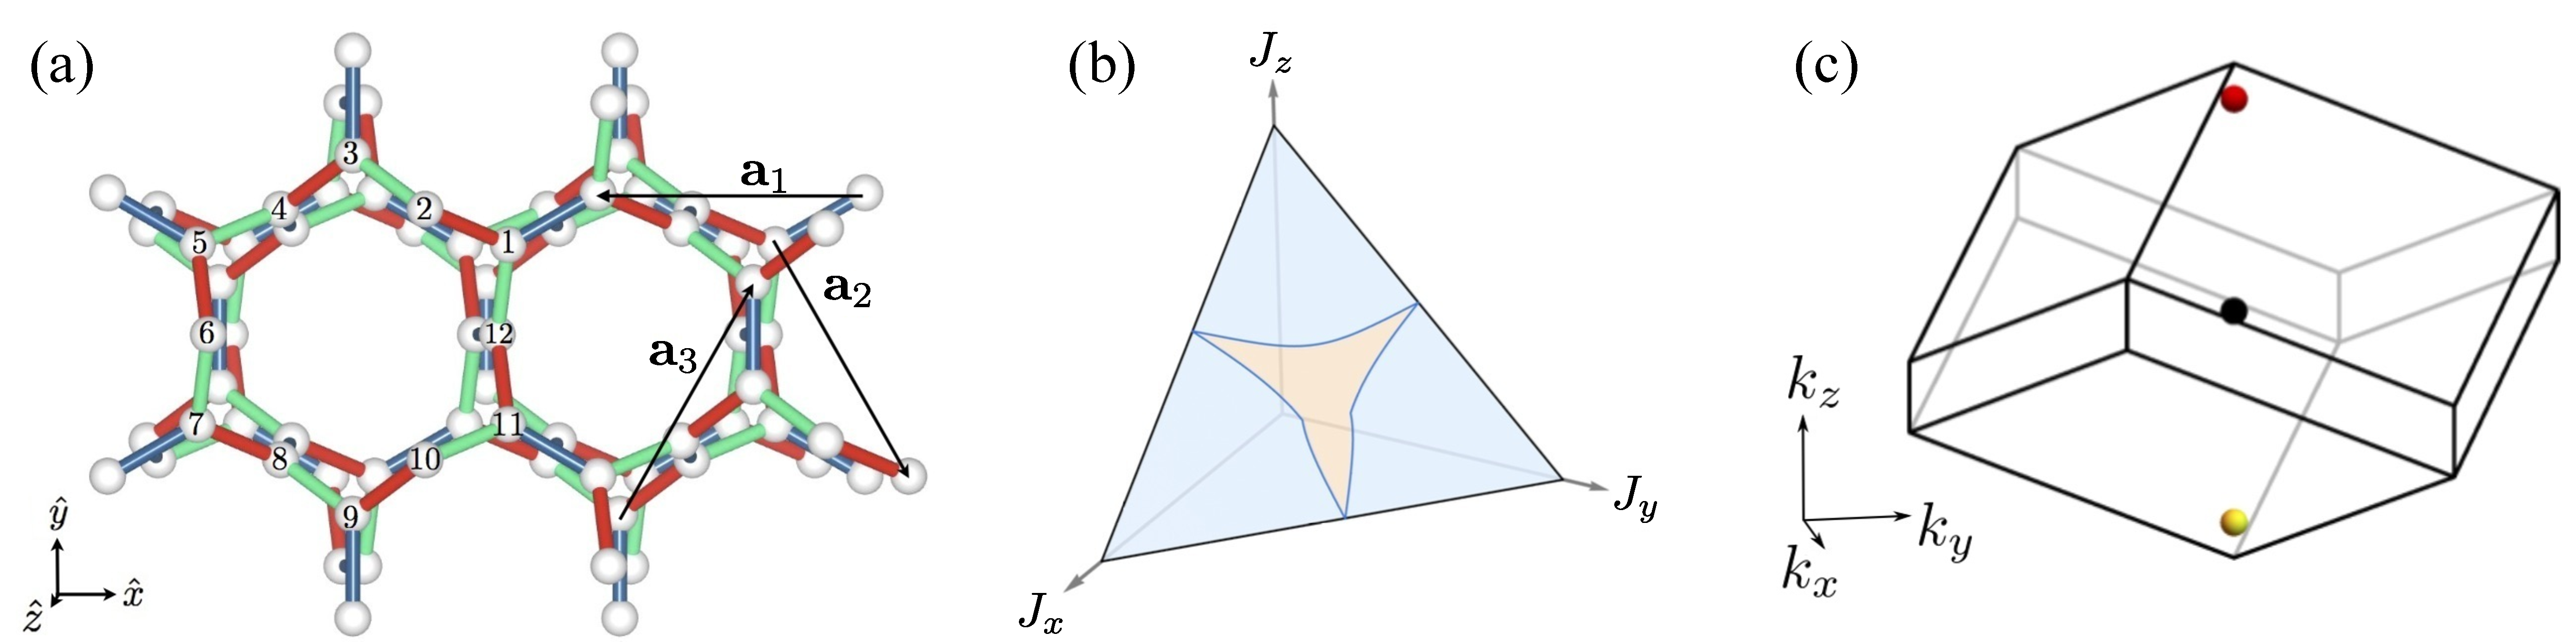
\includegraphics[width=\linewidth]{./chapter05/9_3aPanel.pdf}
	\caption{
		(a) Unit cell and translation vectors for the Kitaev model on lattice (9,3)a.
		(b) Phase diagram for lattice (9,3)a.
		The orange shaded region correspond to a gapless Weyl spin liquid phase.
		The blue shaded regions are gapped.
		(c) Brillouin zone with positions of the Weyl nodes for isotropic exchange couplings.
		Positive and negative Weyl nodes are colored red and yellow, respectively.
		A neutral combination of several Weyl nodes is denoted in black at the $\Gamma$-point.
	}
	\label{fig:chapter05_9_3aPanel}
\end{figure}
%


%
%
\subsubsection{Gauge structure}
%
%
Recalling the definition of the loop operators
%
\begin{equation}
\op{W}_p = -\prod_{\avg{j,k} \in p} (-i \sigma^{\gamma}_j \sigma^{\gamma}_k),
\end{equation}
%
one notes that for loops $p$ of odd length (as found in any \textit{non}-bipartite lattice), the corresponding loop operator is odd under time-reversal.
As a result, any eigenstate of the Kitaev Hamiltonian in a fixed flux sector breaks time-reversal symmetry spontaneously.
All eigenstates, therefore, come in degenerate time-reversal pairs with opposite $\pm \pi/2$-flux threaded through the odd-length loops.
A very similar scenario was explored in Reference~\cite{YaoPRL2007} in the discussion of a chiral spin liquid ground state emerging for a two-dimensional Kitaev model on the 3-12-12 lattice.

Lattice (9,3)a has eight loops of length 9 and one loop of length 12 per unit cell.
These nine loop operators may be combined to form two closed volumes, each of which shares a loop of length 12, leading to only \textit{six} independent loop operators of length 9 per unit cell (see Figure~\ref{fig:chapter05_9_3aPanel2} and Appendix~\ref{appendix:ThreeDimensionalKitaevModels_9_3a} for details).
In order to meaningfully discuss the \ZZ-flux of odd-length loops, one must define an orientation for the loop.
The convention used here will be to consider the loop as the boundary of an oriented surface whose normal points out of the closed volume of which it is a part.

There are only two flux configurations (not including their respective time-reversal partners) which respect the $C_3$, inversion and translations symmetries of the lattice.
These two configurations differ in that one configuration assigns $0$-flux to the loop of length 12 whereas the other assigns $\pi$-flux to the loop (see Figure~\ref{fig:chapter05_9_3aPanel2}~(b) and (c) for a visualization).
It turns out that the $0$-flux configuration has the lower energy of the two and is the flux sector which is studied in this section.
However, this $0$-flux configuration was always known \textit{not} to be the ground state flux configuration.
Unfortunately, in order to accommodate these symmetric flux sectors, the gauge field requires an enlargement of the unit cell to 96 sites, which, at the time of the publication of Reference~\cite{OBrienPRB2016} which this chapter is based off of, posed a challenge to performing a proper finite size analysis.

Subsequently, a quantum Monte Carlo study~\cite{MischenkoPRB2019} was performed to determine the ground state phase diagram for lattice (9,3)a.
It turns out that the ground state flux configuration depends greatly on the relative strengths of the exchange couplings.
The results of this study are the subject of Chapter~\ref{chapter:HypernonagonLattice}.
The vison gap for lattice (9,3)a is not reported here as calculations were not done in the ground state sector, however, it is worth noting that an elementary vison excitation results in the excitation of four loop operators (further details are given in Appendix~\ref{appendix:ThreeDimensionalKitaevModels_9_3a}).
%
\begin{figure}[tb]
	\centering
	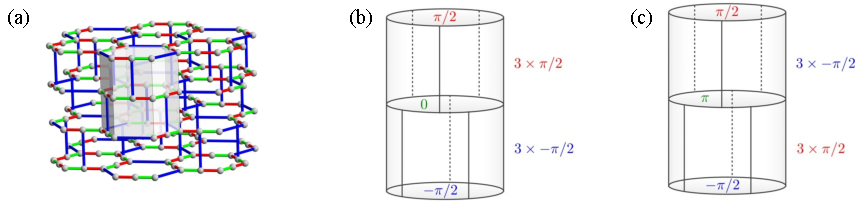
\includegraphics[width=\linewidth]{./chapter05/9_3aPanel2.pdf}
	\caption{
		(a) A deformed version of lattice (9,3)a can be obtained by coupling honeycomb layers via mid-bond sites.
		The eight elementary plaquettes of length nine per unit cell are marked by the gray transparent polygons.
		(b) $0$-flux assignment.
		(c) $\pi$-flux assignment.
	}
	\label{fig:chapter05_9_3aPanel2}
\end{figure}
%


%
%
\subsubsection{Projective symmetries}
%
%
Lattice (9,3)a is the only non-bipartite lattice considered in this project.
As such, there is no projective-representation of the time-reversal operator as time-reversal symmetry is broken on the level of the physical flux sector.
The lattice is inversion symmetric with projective representation
%
\begin{equation}
	H(\bk) = G\dag_{\mathcal{P}}~U_{\mathcal{P}}~H(-\bk)~U\dag_{\mathcal{P}}~G_{\mathcal{P}},
\end{equation}
%
where $U_{\mathcal{P}}$ is the matrix representation of the inversion operator acting on the unit cell and $G_\mathcal{P}$ is the associated gauge transformation.
The resulting energy relations are given by
%
\begin{equation}
	E_{\alpha}(\bk) = -E_{\beta}(-\bk) \qquad {\rm and } \qquad E_{\alpha}(\bk) = E_{\gamma}(-\bk),
\end{equation}
%
due to particle-hole and inversion symmetry, respectively.
Due to the lack of a projective time-reversal operator, the momentum space Hamiltonian matrix has the general form
%
\begin{equation}
	H(\bk) =
		\begin{pmatrix}
			0			&	&	A(\bk) \\
						& \ddots & \\
			A\dag(\bk)	&		 & 0
		\end{pmatrix},
\end{equation}
%
\ie, it is an inversion symmetric band Hamiltonian.


%
%
\subsubsection{Majorana band structure}
%
%
For a fixed momentum $\bk$, the general form of the Hamiltonian $H(\bk)$ for lattice (9,3)a is identical to that of lattice (8,3)b, \ie, a generic, inversion symmetric band Hamiltonian.
Just like in lattice (8,3)b, this prohibits the formation of stable Fermi surfaces, but allows for Weyl nodes pinned to zero energy.
Unlike in lattice (8,3)b, however, the Weyl nodes are not related by time-reversal symmetry.

Indeed, diagonalizing the concrete Hamiltonian for lattice (9,3)a reveals an extended gapless Weyl spin liquid phase around the point of isotropic couplings (see phase diagram in Figure~\ref{fig:chapter05_9_3aPanel}~(b)).
At the isotropic point, there are double Weyl nodes located at the positions $\pm(\bq_1 + \bq_2 + \bq_3)/3$ with charge $\mp 2$ as shown in Figure~\ref{fig:chapter05_9_3aPanel}~(c).
The fourfold degeneracy of these points is protected by the combination of particle-hole and inversion symmetries and, thus, is not affected by the addition of an external magnetic field.
Additionally, there is an eightfold degeneracy at the $\Gamma$-point consisting of a charge-neutral combination of several Weyl nodes.


%
%
% LATTICE (10,3)A %%%%%%%%%%%%%%%%%%%%%%%%%%%%%%%%%%%%%%%%%%%%%%%%%%%%%%%%%%%%%%%%%%%%%%
\subsection{Lattice (10,3)a}
\label{section:chapter05_10_3a}
%%%%%%%%%%%%%%%%%%%%%%%%%%%%%%%%%%%%%%%%%%%%%%%%%%%%%%%%%%%%%%%%%%%%%%%%%%%%%%%%%%%%%%%%
%
%
\subsubsection{Lattice information}
%
%
Lattice (10,3)a (also known in the literature as the Laves graph~\cite{HeeschZFK1933}, $K_4$ crystal~\cite{SunadaAMS2008} or hyperoctagon lattice~\cite{HermannsPRB2014}) has been previously discussed in the context of Kitaev spin liquids in Reference~\cite{HermannsPRB2014} and will be reviewed in this section.
This lattice may be viewed as another three-dimensional variant of the square-octagon lattice, wherein squares and octagons form counter-rotating spirals to form a three-dimensional lattice.
More formally, lattice (10,3)a is specified by the cubic space group $I4_{1}32$ (No. 214) and Wyckoff positions for the unit cell are $8(a)$.
The concrete choice of four site unit cell used in this work is given by the site positions
%
\begin{equation}
	\begin{matrix*}[l]
		\br_1 = \left(\frac{1}{8}, \frac{1}{8}, \frac{1}{8}\right) &
		\br_2 = \left(\frac{5}{8}, \frac{3}{8}, -\frac{1}{8}\right) \\
		&\\
		\br_3 = \left(\frac{3}{8}, \frac{1}{8}, -\frac{1}{8}\right) &
		\br_4 = \left(\frac{7}{8}, \frac{3}{8}, \frac{1}{8}\right).
	\end{matrix*}
\end{equation}
%
The lattice vectors are chosen to be
%
\begin{equation}
	\begin{matrix*}[l]
		\ba_1 = \left(1, 0, 0\right) \qquad
		\ba_2 = \left(\frac{1}{2}, \frac{1}{2}, -\frac{1}{2}\right) \qquad
		\ba_3 = \left(\frac{1}{2}, \frac{1}{2}, \frac{1}{2}\right)
	\end{matrix*}
\end{equation}
%
with the corresponding reciprocal lattice vectors
%
\begin{equation}
	\begin{matrix*}[l]
		\bq_1 = \left(2\pi, -2\pi, 0\right) \qquad
		\bq_2 = \left(0, 2\pi, -2\pi\right) \qquad
		\bq_3 = \left(0, 2\pi, 2\pi\right).
	\end{matrix*}
\end{equation}
%

The unit cell and translation vectors are illustrated in Figure~\ref{fig:chapter05_10_3aPanel}~(a).
The bonds are colored red, green and blue to indicate the assignment of $x$-, $y$- and $z$-type bonds, respectively.
This assignment of bonds is chosen to respect as many lattice symmetries as possible.
All $x$-, $y$- and $z$-bonds are related by a combination of $C_3$ and a fourfold screw symmetry.
The symmetry between $x$-, $y$- and $z$-bonds is reflected in the ground state phase diagram shown in Figure~\ref{fig:chapter05_10_3aPanel}~(b).
%
\begin{figure}[tb]
	\centering
	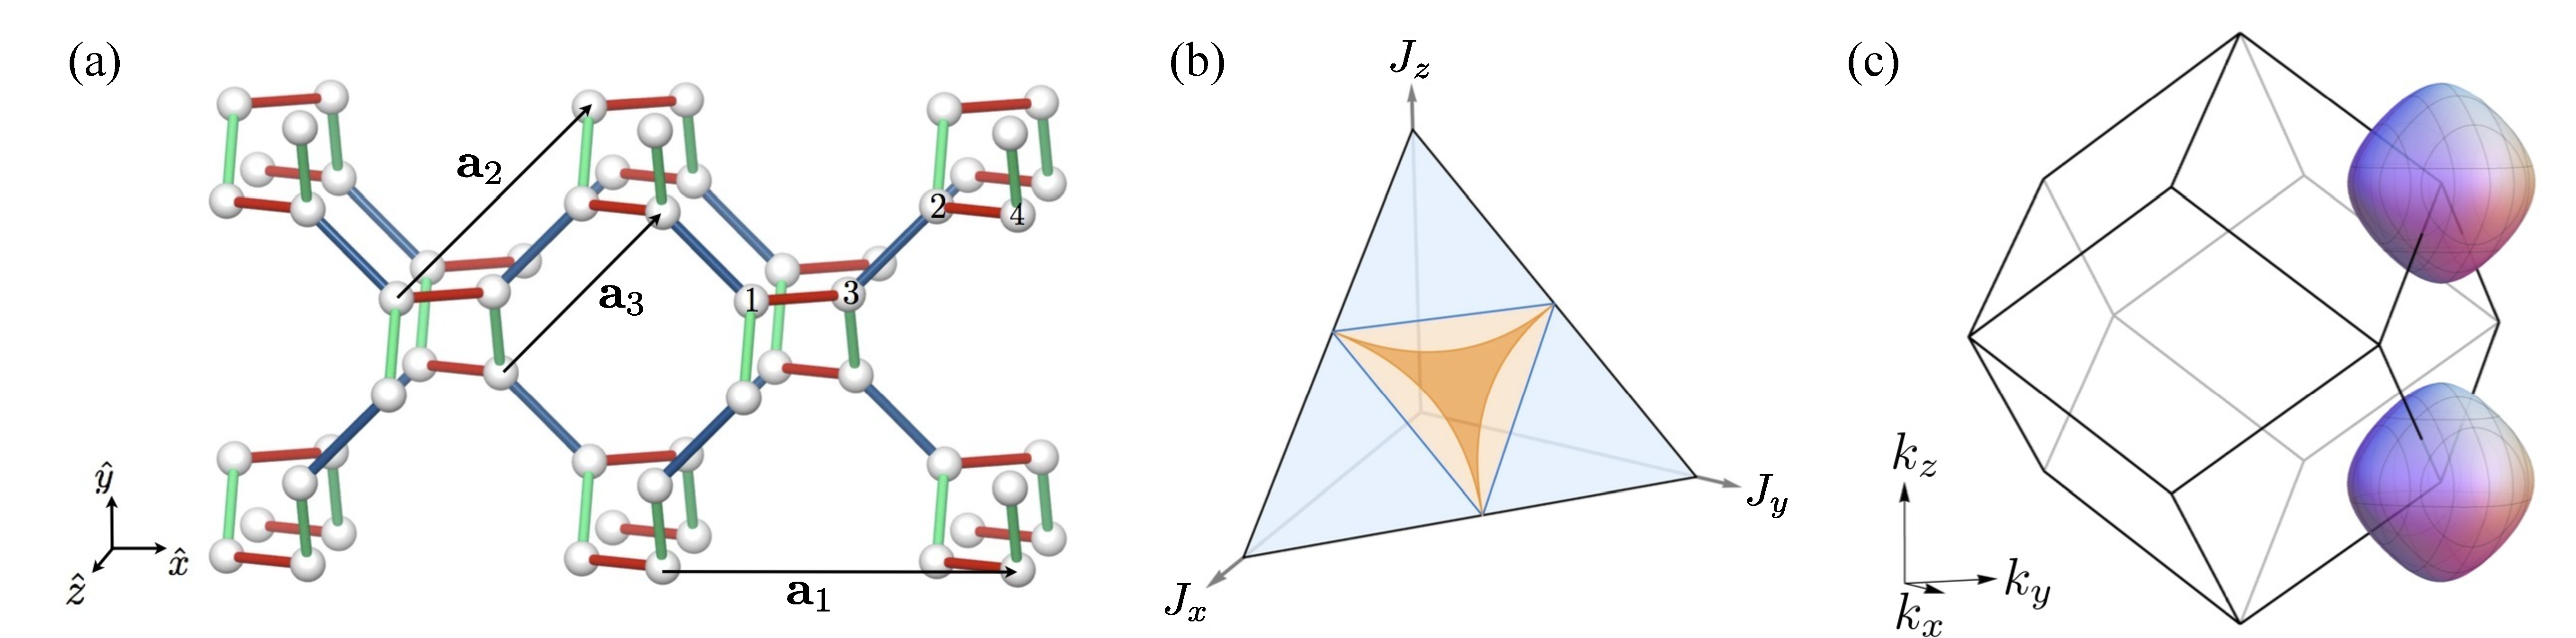
\includegraphics[width=\linewidth]{./chapter05/10_3aPanel.pdf}
	\caption{
		(a) Unit cell and translation vectors for the Kitaev model on lattice (10,3)a.
		(b) Ground state phase diagram for lattice (10,3)a.
		The region shaded darker orange has topological Fermi surfaces while the lighter orange regions have topologically-trivial Fermi surfaces.
		The blue shaded regions are gapped.
		(c) Visualization of the Majorana Fermi surfaces for isotropic exchange couplings.
	}
	\label{fig:chapter05_10_3aPanel}
\end{figure}
%


%
%
\subsubsection{Gauge structure}
%
%
Lattice (10,3)a possesses six loop operators of length 10 per unit cell.
These six loop operators may be combined to form four closed volumes leading to only \textit{two} independent loop operators per unit cell (see Appendix~\ref{appendix:ThreeDimensionalKitaevModels_10_3a} for details).
The canonical flux sector for lattice (10,3)a corresponds to $0$-flux through all elementary loops.
This results in all loop operators $\op{W}_p$ having eigenvalues $+1$.
Additionally, it has been checked numerically that the canonical flux sector is, indeed, the ground state flux sector.
The vison gap for lattice (10,3)a shown in Figure~\ref{fig:chapter05_VisonGaps}~and Table~\ref{table:chapter05_VisonGaps}~has been computed by flipping the value of $u_{jk}$ for a single $z$-bond, resulting in the excitation of ten loop operators (further details are given in Appendix~\ref{appendix:ThreeDimensionalKitaevModels_10_3a}).


%
%
\subsubsection{Projective symmetries}
%
%
Lattice (10,3)a is bipartite with different sublattices connected by the vectors $\br_0 = \ba_2$ and $\br'_0 = \ba_3$.
As a result, the projective representation of time-reversal is given by
%
\begin{equation}
	H(\bk) = G\dag_{\mathcal{T}}~H(-\bk + \bk_0)~G_{\mathcal{T}},
\end{equation}
%
where $\bk_0 = (\bq_2 + \bq_3)/2$ and the associated gauge transformation matrix is given by
%
\begin{equation}
	G_{\mathcal{T}} =
	\begin{pmatrix}
		\id	& 0    \\
		0	& -\id
	\end{pmatrix}.
\end{equation}
%
As lattice (10,3)a is chiral, the only other restriction to consider is that of particle-hole symmetry.
The resulting energy relations are given by
%
\begin{equation}
	E_{\alpha}(\bk) = -E_{\beta}(-\bk) \qquad {\rm and } \qquad E_{\alpha}(\bk) = E_{\gamma}(-\bk + \bk_0),
\end{equation}
%
due to particle-hole and time-reversal symmetry, respectively.
Due to the fact that the gauge transformation $\op{G}_{\mathcal{T}}$ relates states at momentum $\bk$ to states at momentum $\bk - \bk_0$, the momentum space Hamiltonian matrix has the form of a generic band Hamiltonian,
%
\begin{equation}
	H(\bk) =
		\begin{pmatrix}
			0			&		 & A(\bk) \\
						& \ddots &		  \\
			A\dag(\bk)	&		 & 0
		\end{pmatrix}.
\end{equation}
%


%
%
\subsubsection{Majorana band structure}
%
%
As discussed in the context of lattice (8,3)a, due to the non-trivial projective representation of time-reversal symmetry, \ie, with $\bk \neq \bm{0}$, along with the absence of inversion symmetry, lattice (10,3)a may host topological Fermi surfaces protected by Weyl-type degeneracies at finite energy.
Indeed, diagonalizing the concrete Kitaev Hamiltonian for lattice (10,3)a reveals an extended gapless phase around the point of isotropic couplings.
In the phase diagram of Figure~\ref{fig:chapter05_10_3aPanel}~(b), the darker shaded orange region corresponds to the presence of such topologically protected Fermi surfaces, whereas the lighter shaded orange regions correspond to topologically trivial Fermi surfaces.
%
\begin{figure}[tb]
	\centering
	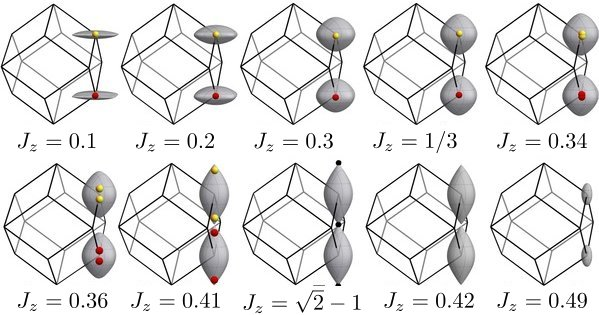
\includegraphics[width=0.55\linewidth]{./chapter05/10_3aFermiSurface.png}
	\caption{
		Evolution of the Majorana Fermi surfaces of lattice (10,3)a for varying exchange couplings $0.1 \leq J_z \leq 0.49$ and $J_x = J_y = (1 - Jz)/2$.
	}
	\label{fig:chapter05_10_3aFermiSurfaces}
\end{figure}
%

The topological Fermi surfaces are protected by Weyl-like degeneracies at finite energy.
There are a total of four such Weyl points, two of which are positively charged and two of which are negatively charged.
The four Weyl points are formed by only three bands and each Fermi surface contains two Weyl points of the same chirality.
At the isotropic point, where the Hamiltonian is highly-symmetric, pairs of Weyl points of the same chirality sit at the same momentum resulting in a threefold degeneracy which has been seen to correspond to a so-called spin-1 Weyl point~\cite{WawrzikPRB2018}.
As the couplings are tuned away from the isotropic point, however, the Weyl points are free to move through the Brillouin zone, deforming the Fermi surfaces as they do so.
Eventually, Weyl points of opposite chirality meet at high-symmetry points and mutually annihilate as the Fermi surfaces touch, thus, removing the topological protection of the Fermi surfaces.
Tuning the couplings further ultimately shrinks the Fermi surfaces to a point before gapping them out entirely (refer to Figure~\ref{fig:chapter05_10_3aFermiSurfaces} for a visualization).

The two Majorana Fermi surfaces can be mapped onto each other by the perfect nesting vector $\bk_0$ as can be seen from Figure~\ref{fig:chapter05_10_3aPanel}~(c).
As a result, the system is susceptible to a BCS-type spin-Peierls instability~\cite{HermannsPRL2015b} driven by interactions between the Majorana fermions, which can be induced by additional spin exchange such as a Heisenberg term.
A short discussion of the spin-Peierls instability occurs in Section~\ref{section:chapter05_SpinPeierls}.

Breaking time-reversal symmetry by applying an external magnetic field does not qualitatively change the nature of the nodal manifold, \ie, they remain Fermi surfaces.
However, they do deform in a non-trivial way as magnetic field strength is varied, destroying the perfect nesting condition (see Figure~\ref{fig:chapter05_10_3aPanel2}).
%
\begin{figure}[tb]
	\centering
	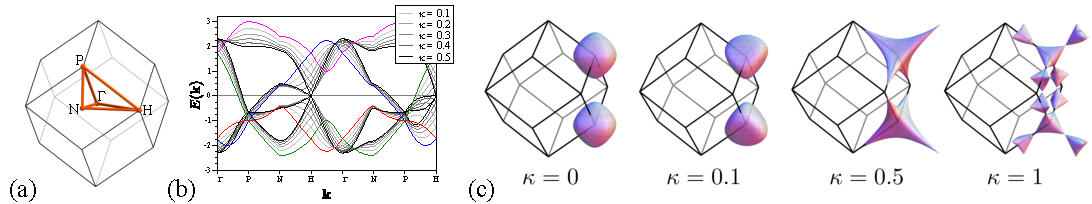
\includegraphics[width=\linewidth]{./chapter05/10_3aPanel2.pdf}
	\caption{
		(a) Brillouin zone of lattice (10,3)a with high-symmetry points.
		(b) Majorana dispersion plotted along the high-symmetry paths for varying $\kappa$.
		(c) Deformation of the Fermi surfaces in the presence of a magnetic field of varying strength $0 \leq \kappa \leq 1$.
	}
	\label{fig:chapter05_10_3aPanel2}
\end{figure}
%


%
%
% LATTICE (10,3)B %%%%%%%%%%%%%%%%%%%%%%%%%%%%%%%%%%%%%%%%%%%%%%%%%%%%%%%%%%%%%%%%%%%%%%
\subsection{Lattice (10,3)b}
\label{section:chapter05_10_3b}
%%%%%%%%%%%%%%%%%%%%%%%%%%%%%%%%%%%%%%%%%%%%%%%%%%%%%%%%%%%%%%%%%%%%%%%%%%%%%%%%%%%%%%%%
%
%
\subsubsection{Lattice information}
%
%
Lattice (10,3)b is probably the best known three-dimensional tricoordinated lattice and is typically referred to in the literature as the hyperhoneycomb lattice~\cite{TakayamaPRL2015}.
The Kitaev model for this lattice has been discussed extensively~\cite{MandalPRB2009,HermannsPRB2014,LeePRB2014,KimchiPRB2014,NasuPRB2014} in the context of the iridate material \betaLithiumIridate~\cite{TakayamaPRL2015}.

The most symmetric form of lattice (10,3)b can best be visualized as parallel $xy$-zigzag chains along two distinct direction which are coupled by $z$-type bonds
It may be viewed as a close relative of lattice (10,3)c which is made up of three parallel $xy$-zigzag chains which are coupled by $z$-type bonds (see Figure~\ref{fig:chapter05_10_3bcComparison} for a comparison).
Formally, lattice (10,3)b is specified by the tetragonal space group $I4_{1}/ambd$ (No. 141) with $c/a = 2\sqrt{3}$ and Wyckoff positions for the unit cell are $8(e)$ with $z = 1/12$.
The concrete choice of four site unit cell used in this work is given by the site positions
%
\begin{equation}
	\begin{matrix*}[l]
		\br_1 = \left(0, 0, 0\right) &
		\br_2 = \left(1, 2, 1\right) \\
		&\\
		\br_3 = \left(1, 1, 0\right) &
		\br_4 = \left(2, 3, 1\right).
	\end{matrix*}
\end{equation}
%
The lattice vectors are chosen to be
%
\begin{equation}
	\begin{matrix*}[l]
		\ba_1 = \left(-1, 1, -2\right) \qquad
		\ba_2 = \left(-1, 1, 2\right) \qquad
		\ba_3 = \left(2, 4, 0\right)
	\end{matrix*}
\end{equation}
%
with the corresponding reciprocal lattice vectors
%
\begin{equation}
	\begin{matrix*}[l]
		\bq_1 = \left(-\frac{2\pi}{3}, \frac{\pi}{3}, -\frac{\pi}{2}\right) \qquad
		\bq_2 = \left(-\frac{2\pi}{3}, \frac{\pi}{3}, \frac{\pi}{2}\right) \qquad
		\bq_3 = \left(\frac{\pi}{3}, \frac{\pi}{3}, 0\right).
	\end{matrix*}
\end{equation}
%

The unit cell and translation vectors are illustrated in Figure~\ref{fig:chapter05_10_3bPanel}~(a).
The bonds in the figure are colored red, green and blue to indicate the assignment of $x$-, $y$- and $z$-type bonds, respectively.
This assignment of bonds is chosen to respect as many of the lattice symmetries as possible.
All $x$- and $y$-bonds are related by a combination of $C_2$ and a two-fold screw symmetry.
All $z$-bonds are related to each other by inversion symmetry, but are not related to any other bond type by lattice symmetries.
The symmetry between $x$- and $y$-bonds is reflected in the ground state phase diagram shown in Figure~\ref{fig:chapter05_10_3bPanel}~(b).
%
\begin{figure}[tb]
	\centering
	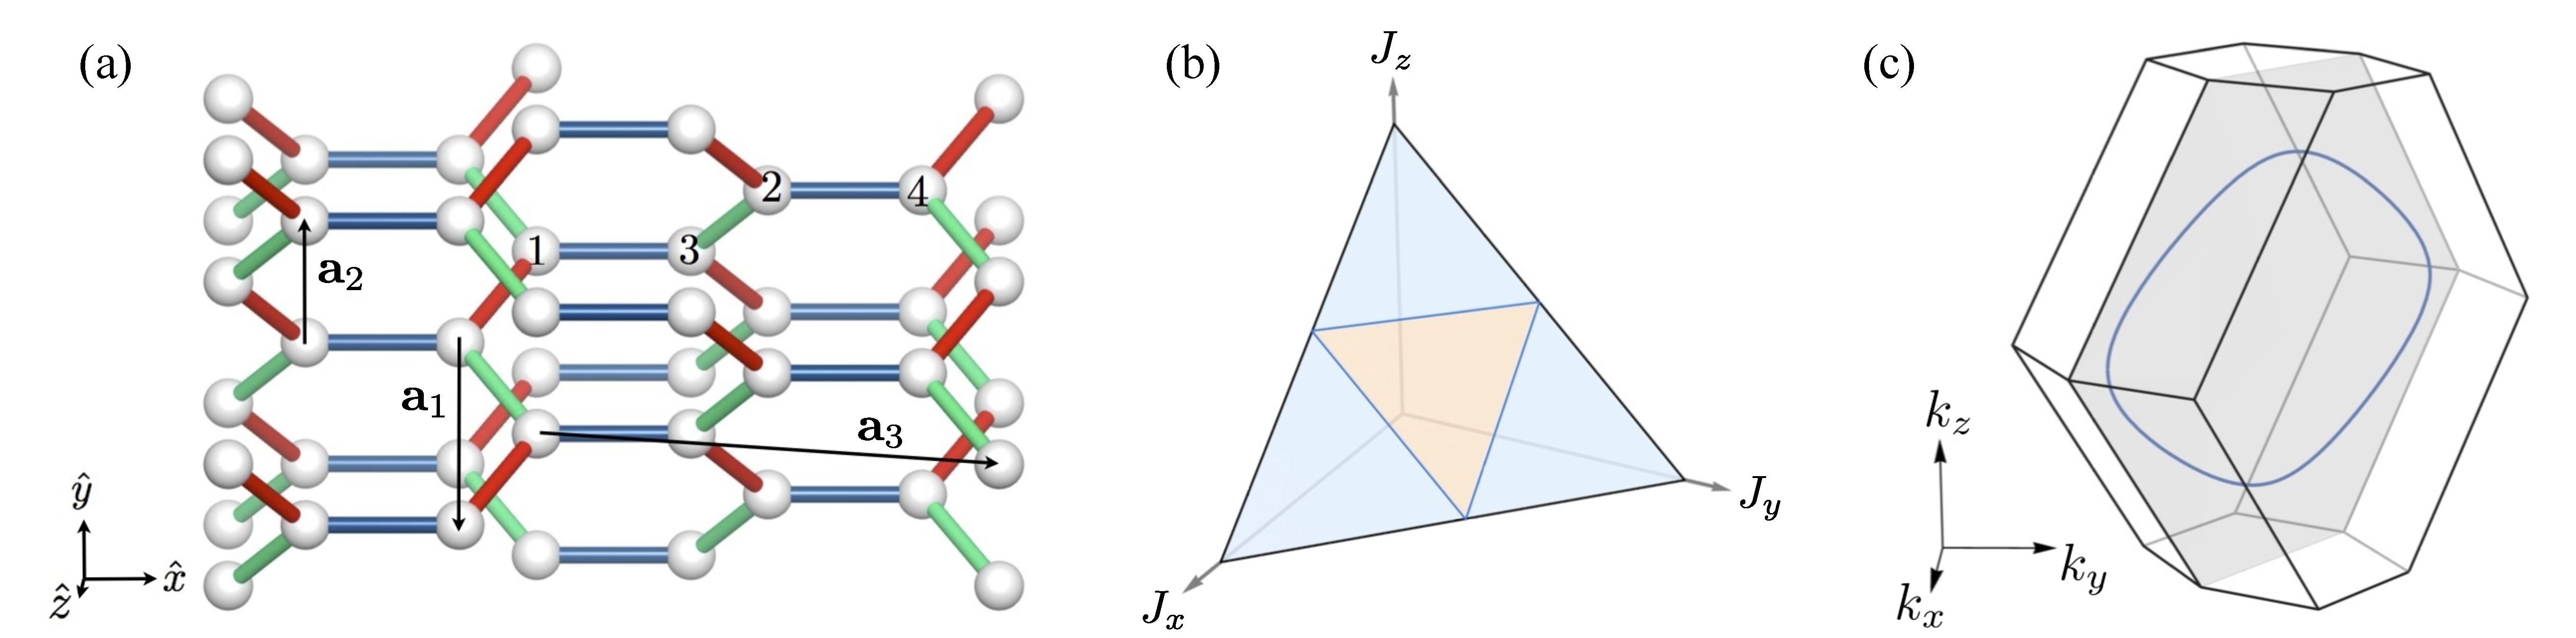
\includegraphics[width=\linewidth]{./chapter05/10_3bPanel.pdf}
	\caption{
		(a) Unit cell and translation vectors for the Kitaev model on lattice (10,3)b.
		(b) Ground state phase diagram for lattice (10,3)b.
		The region shaded orange corresponds to a gapless phase with a nodal line.
		The blue shaded regions are gapped.
		(c) At the isotropic point, the nodal line (marked in blue) is located in the $k_x + k_y = 0$ plane (indicated in gray).
	}
	\label{fig:chapter05_10_3bPanel}
\end{figure}
%


%
%
\subsubsection{Gauge structure}
%
%
Lattice (10,3)b possesses four loop operators of length 10 per unit cell.
These four loop operators can be combined to form two closed volumes, leading to only \textit{two} independent loop operators per unit cell (see Appendix~\ref{appendix:ThreeDimensionalKitaevModels_10_3b} for details).
The canonical flux sector for lattice (10,3)b corresponds to $0$-flux through all elementary loops.
This results in all loop operators $\op{W}_p$ having eigenvalues $+1$.
Additionally, it has been checked numerically that the canonical flux sector is, indeed, the ground state flux sector.
The vison gap for lattice (10,3)b shown in Figure~\ref{fig:chapter05_VisonGaps}~and Table~\ref{table:chapter05_VisonGaps}~has been computed by flipping the value of $u_{jk}$ for a single $z$-bond, resulting in the excitation of six loop operators (further details are given in Appendix~\ref{appendix:ThreeDimensionalKitaevModels_10_3b}).


%
%
\subsubsection{Projective symmetries}
%
%
%
\begin{figure}[tb]
	\centering
	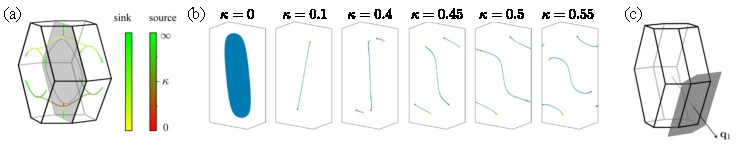
\includegraphics[width=\linewidth]{./chapter05/10_3bPanel2.pdf}
	\caption{
		(a) Evolution of Weyl nodes of lattice (10,3)b in the presence of a magnetic field of varied strength $0 \leq \kappa < \infty$.
		(b) Corresponding Fermi arc evolution.
		(c) Visualization of the surface Brillouin zone for the 100-surface.
	}
	\label{fig:chapter05_10_3bPanel2}
\end{figure}
%
Lattice (10,3)b is bipartite with sublattices having the same translation symmetry as the elementary unit cell.
The resulting projective representation of time-reversal is given by
%
\begin{equation}
	H(\bk) = G\dag_{\mathcal{T}}~H(-\bk)~G_{\mathcal{T}},
\end{equation}
%
where the associated gauge transformation matrix is given by
%
\begin{equation}
	G_{\mathcal{T}} =
		\begin{pmatrix}
			\id & 0 \\
			0	& -\id
		\end{pmatrix}.
\end{equation}
%
Furthermore, the lattice is inversion symmetric with projective representation
%
\begin{equation}
	H(\bk) = G\dag_{\mathcal{P}}~U_{\mathcal{P}}~H(-\bk)~U\dag_{\mathcal{P}}~G_{\mathcal{P}},
\end{equation}
%
where $U_{\mathcal{P}}$ is the matrix representation of the inversion operator acting on the unit cell, and the associated gauge transformation matrix $G_{\mathcal{P}}$ is identical to $G_{\mathcal{T}}$ for the gauge \textit{Ansatz} used here.
The resulting energy relations are given by
%
\begin{equation}
	E_{\alpha}(\bk) = -E_{\beta}(-\bk) \qquad {\rm and } \qquad E_{\alpha}(\bk) = E_{\gamma}(-\bk),
\end{equation}
%
where the first relation is due to particle-hole symmetry and the second is enforced individually by both time-reversal and inversion symmetry.
Due to the fact that the gauge transformation $\op{G}_{\mathcal{T}}$ is constant as a function of unit cell position, the momentum space Hamiltonian matrix has the block off-diagonal form
%
\begin{equation}
	H(\bk) =
		\begin{pmatrix}
			0			& A(\bk) \\
			A\dag(\bk)	& 0
		\end{pmatrix}.
\end{equation}
%
\newpage


%
%
\subsubsection{Majorana band structure}
%
%
As was the case for lattice (8,3)c, a trivially implemented projective time-reversal symmetry leads to nodal lines being the only stable zero energy manifolds for lattice (10,3)b.
These nodal lines are characterized by an integer invariant and are protected by the presence of time-reversal symmetry.

Diagonalizing the concrete Kitaev Hamiltonian for lattice (10,3)b, indeed, reveals an extended gapless phase around the point of isotropic couplings (see Figure~\ref{fig:chapter05_10_3bPanel}~(b)), where the zero modes correspond to a contractible loop in the Brillouin zone.
At the isotropic point, this line lies in the plane defined by $k_x + k_y = 0$.

Breaking time-reversal explicitly by introducing an external magnetic field removes the symmetry protection of the nodal line, gapping it to a pair of Weyl nodes due to the presence of a trivially implemented projective inversion symmetry.
This is precisely the scenario which was seen to occur for lattice (8,3)c, above.
For small values of $\kappa$, the Weyl nodes move along the $z$-axis.
At $\kappa = \frac{1}{2} \sqrt{\frac{3}{5}}$, four more Weyl nodes appear.
The full evolution of the Weyl nodes for $0 \leq \kappa < \infty$ along with the corresponding Fermi arc surfaces states are pictured in Figure~\ref{fig:chapter05_10_3bPanel2}~(a) and (b).
The trajectory of negatively charged Weyl nodes changes colors from yellow to green as $\kappa$ is increased, whereas the trajectory of positively charged Weyl nodes changes from red to green.
While the Weyl nodes which move along the $z$-axis recombine at $\kappa \rightarrow \infty$, the ones on the front/back faces of the Brillouin zone do not.
Instead, the velocity vectors of the isolated Weyl nodes vanish, collapsing the bulk gap to a nodal line.
Additionally, one notes that for the pure Kitaev model, \ie, with $\kappa = 0$, there is an entire puddle of zero modes which appear in the surface Brillouin zone.
These zero modes appear within the area bounded by the projection of the bulk nodal line to the surface Brillouin zone and are associated to the non-vanishing integer invariant due to the presence of time-reversal symmetry.


%
%
% LATTICE (10,3)C %%%%%%%%%%%%%%%%%%%%%%%%%%%%%%%%%%%%%%%%%%%%%%%%%%%%%%%%%%%%%%%%%%%%%%
\subsection{Lattice (10,3)c}
\label{section:chapter05_10_3c}
%%%%%%%%%%%%%%%%%%%%%%%%%%%%%%%%%%%%%%%%%%%%%%%%%%%%%%%%%%%%%%%%%%%%%%%%%%%%%%%%%%%%%%%%
%
%
\subsubsection{Lattice information}
%
%
As mentioned above lattice (10,3)c is in some sense a relative of lattice (10,3)b (see discussion at the beginning of Section~\ref{section:chapter05_10_3b} and Figure~\ref{fig:chapter05_10_3bcComparison}).
One significant distinction between the two lattices is that, whereas lattice (10,3)b is inversion symmetric, lattice (10,3)c is chiral.
%
\begin{figure}[tb]
	\centering
	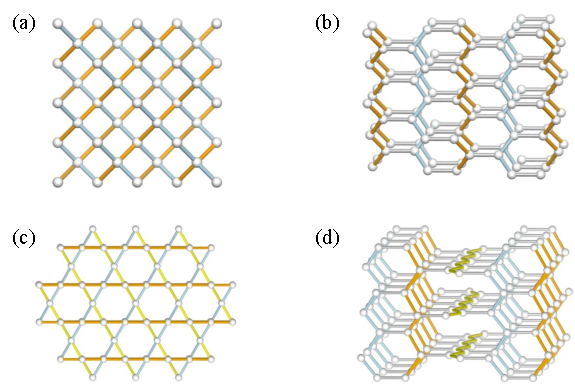
\includegraphics[width=0.6\linewidth]{./chapter05/10_3bcComparison.pdf}
	\caption{
		Comparison of lattice (10,3)b -- shown in (a) and (b) -- and lattice (10,3)c -- shown in (c) and (d).
	}
	\label{fig:chapter05_10_3bcComparison}
\end{figure}
%

More formally, lattice (10,3)c is specified by the trigonal space group $P3_{1}12$ (No. 151) with $c/a = 3\sqrt{3}/2$ and Wyckoff positions for the unit cell are $6(c)$ with $x = 1/3$, $y = 1/6$ and $z = 1/9$.
The concrete choice of unit cell specified in this work has six sites per unit cell at positions
%
\begin{equation}
	\begin{matrix*}[l]
		\br_1 = \left(\frac{1}{4}, \frac{1}{4\sqrt{3}}, \frac{1}{2\sqrt{3}}\right) &
		\br_2 = \left(\frac{3}{4}, \frac{1}{4\sqrt{3}}, \frac{2}{\sqrt{3}}\right) &
		\br_3 = \left(\frac{1}{2}, \frac{1}{\sqrt{3}}, \frac{7}{2\sqrt{3}}\right) \\
		&\\
		\br_4 = \left(\frac{3}{4}, \frac{1}{4\sqrt{3}}, \frac{1}{\sqrt{3}}\right) &
		\br_5 = \left(\frac{1}{2}, \frac{1}{\sqrt{3}}, \frac{5}{2\sqrt{3}}\right) &
		\br_6 = \left(\frac{1}{4}, \frac{1}{4\sqrt{3}}, \frac{4}{\sqrt{3}}\right).
	\end{matrix*}
\end{equation}
%
The lattice vectors are chosen to be
%
\begin{equation}
	\begin{matrix*}[l]
		\ba_1 = \left(1, 0, 0\right) \qquad
		\ba_2 = \left(-\frac{1}{2}, \frac{\sqrt{3}}{2}, 0\right) \qquad
		\ba_3 = \left(0, 0, \frac{3\sqrt{3}}{2}\right)
	\end{matrix*}
\end{equation}
%
with the corresponding reciprocal lattice vectors
%
\begin{equation}
	\begin{matrix*}[l]
		\bq_1 = \left(2\pi, \frac{2\pi}{\sqrt{3}}, 0\right) \qquad
		\bq_2 = \left(0, \frac{4\pi}{\sqrt{3}}, 0\right) \qquad
		\bq_3 = \left(0, 0, \frac{4\pi}{3\sqrt{3}}\right).
	\end{matrix*}
\end{equation}
%
As will be discussed in the following section, this unit cell must be enlarged in order to accommodate the ground state flux sector.

The unit cell and translation vectors are illustrated in Figure~\ref{fig:chapter05_10_3cPanel}~(a).
The bonds in the figure are colored red, green and blue, to indicate the assignment of $x$-, $y$- and $z$-type bonds, respectively.
This assignment of bonds is chosen to respect as many of the lattice symmetries as possible.
All $x$- and $y$-bonds are related by a threefold screw symmetry.
All $z$-bonds are related to each other by the same screw symmetry, but not to any other type of bond.
The symmetry between $x$- and $y$-bonds is reflected in the ground state phase diagram shown in Figure~\ref{fig:chapter05_10_3cPanel}~(b).


%
%
\subsubsection{Gauge structure}
%
%
Lattice (10,3)c possesses three loop operators of length 10 and three of length 12 per unit cell.
These six loop operators can be combined to form three closed volumes, leading to only \textit{three} independent loop operators per unit cell (see Appendix~\ref{appendix:ThreeDimensionalKitaevModels_10_3c} for details).
The canonical flux sector for lattice (10,3)c corresponds to $0$-flux through all loops of length 10 and $\pi$-flux through all loops of length 12.
This results in all loop operators $\op{W}_p$ having eigenvalues $+1$.
Additionally, it has been checked numerically that the canonical flux sector is, indeed, the ground state flux sector.
In order to fix a gauge \textit{Ansatz} compatible with the ground state flux sector, however, the unit cell must be doubled in the 010-direction (see Appendix~\ref{appendix:ThreeDimensionalKitaevModels_10_3c} for definition of the expanded unit cell).
The vison gap for lattice (10,3)c shown in Figure~\ref{fig:chapter05_VisonGaps}~and Table~\ref{table:chapter05_VisonGaps}~has been computed by flipping the value of $u_{jk}$ for a single $z$-bond, resulting in the excitation of fourteen loop operators (further details are given in Appendix~\ref{appendix:ThreeDimensionalKitaevModels_10_3c}).
%
\begin{figure}[tb]
	\centering
	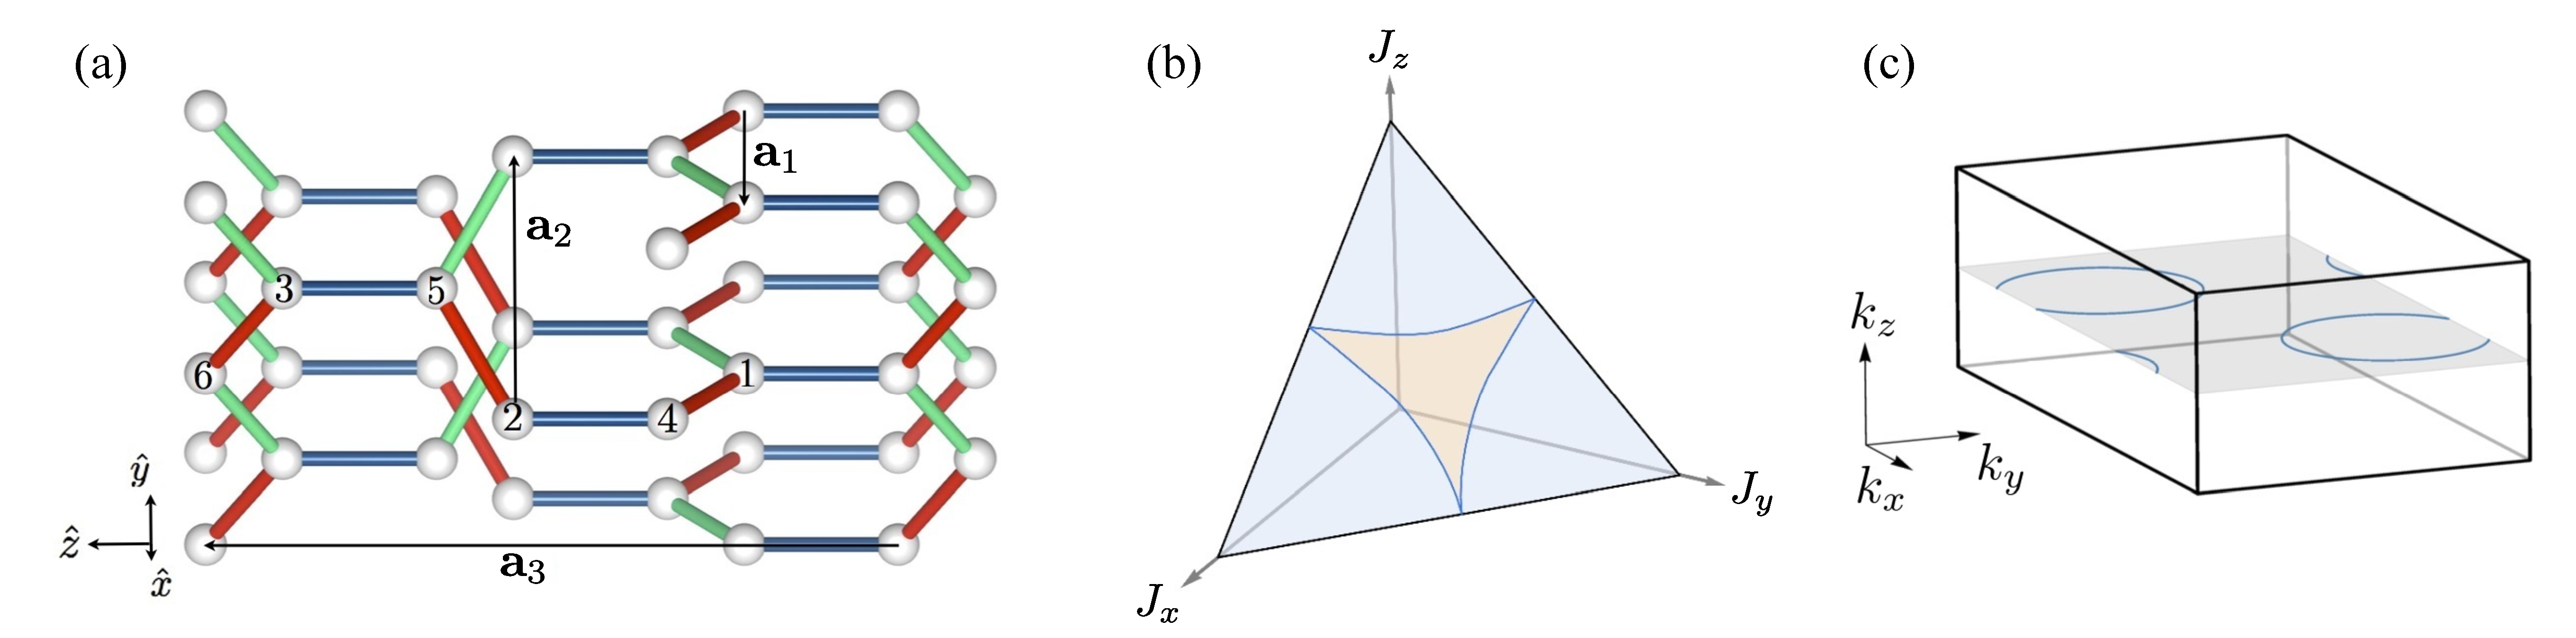
\includegraphics[width=\linewidth]{./chapter05/10_3cPanel.pdf}
	\caption{
		(a) Unit cell and translation vectors for the Kitaev model on lattice (10,3)c.
		(b) Ground state phase diagram for lattice (10,3)c.
		The region shaded orange corresponds to a gapless phase with nodal lines.
		The blue shaded regions are gapped.
		(c) At the isotropic point, the nodal lines (marked in blue) are located in the $k_z = 0$ plane (indicated in gray).
	}
	\label{fig:chapter05_10_3cPanel}
\end{figure}
%


%
%
\subsubsection{Projective symmetries}
%
%
Lattice (10,3)c is bipartite with sublattices having the same translation symmetry as the elementary unit cell.
The resulting projective representation of time-reversal is given by
%
\begin{equation}
	H(\bk) = G\dag_{\mathcal{T}}~H(-\bk)~G_{\mathcal{T}},
\end{equation}
%
where the associated gauge transformation matrix is given by
%
\begin{equation}
	G_{\mathcal{T}} =
		\begin{pmatrix}
			\id & 0 \\
			0	& -\id
		\end{pmatrix}.
\end{equation}
%
As mentioned above, the gauge \textit{Ansatz} in the canonical flux sector necessarily doubles the unit cell in the 010-direction, resulting in a gauge \textit{Ansatz} which is not \textit{invariant} under translations along $\ba_2$.
It is, however, \textit{symmetric} under translations along $\ba_2$ when the corresponding gauge transformation is accounted for.
This gauge transformation alternates in sign as a function of unit cell position $\br$ in the $\ba_1$ direction, \ie,
\begin{align}
	G_{T_2}(\br) &= -G_{T_2}(\br + \ba_1) \nonumber\\
				 &= \exp{(i \bk'_0 \cdot \br)} G_{T_2}(\br),
\end{align}
where $\bk'_0 = \bq_1 / 2$.
As lattice (10,3)c is chiral, the only other restriction to consider is that of particle-hole symmetry.
The resulting energy relations are given by
%
\begin{equation}
	E_{\alpha}(\bk) = - E_{\beta}(-\bk) \qquad E_{\alpha}(\bk) = E_{\gamma}(-\bk) \qquad E_{\alpha}(\bk) = E_{\delta}(\bk + \bk'_0),
\end{equation}
%
due to particle-hole, time-reversal and translation symmetry, respectively.
Due to the fact that the gauge transformations $\op{G}_{\mathcal{T}}$ is constant as a function of unit cell position, the momentum space Hamiltonian matrix has the block off-diagonal form
%
\begin{equation}
	H(\bk) =
		\begin{pmatrix}
			0			& A(\bk) \\
			A\dag(\bk)	& 0
		\end{pmatrix}.
\end{equation}
%


%
%
\subsubsection{Majorana band structure}
%
%
As was the case for lattices (8,3)c and (10,3)b, a trivially implemented projective time-reversal symmetry leads to nodal lines being the only stable zero energy manifolds for lattice (10,3)c.
These nodal lines are characterized by an integer invariant and are protected by the presence of time-reversal symmetry.

Diagonalizing the concrete Kitaev Hamiltonian for lattice (10,3)c, indeed, reveals an extended gapless phase around the point of isotropic couplings (see Figure~\ref{fig:chapter05_10_3cPanel}~(b)), where the zero modes correspond to two closed nodal lines.
These nodal lines are related by the nesting vector $\bk'_0 = \bq_1 / 2$ due to the projective representation of translation symmetry.
For isotropic couplings, these nodal lines lie in the plane defined by $k_z = 0$ (see Figure~\ref{fig:chapter05_10_3cPanel}~(c) -- note that the Brillouin zone is for the expanded unit cell).
Breaking time-reversal symmetry explicitly by introducing an external magnetic field removes the symmetry protection of the nodal lines, gapping each line to six Weyl nodes related by a threefold screw axis, for a total of twelve Weyl nodes.

However, in contrast to lattices (8,3)c and (10,3)b, lattice (10,3)c is chiral.
This lack of inversion symmetry allows the Weyl-degeneracies to move away from zero energy as $\kappa$ is increased, resulting in twelve Fermi surfaces.
As each Fermi surface is generated by a Weyl-like degeneracy, it inherits a topological protection.
For a visualization of the formation of the Fermi surfaces, refer to Figure~\ref{fig:chapter05_10_3cPanel2}.
Note that lattice (10,3)c represents the only example presented in this work for which the breaking of time-reversal symmetry actually \textit{increases} the density of states at zero energy.
%
\begin{figure}[tb]
	\centering
	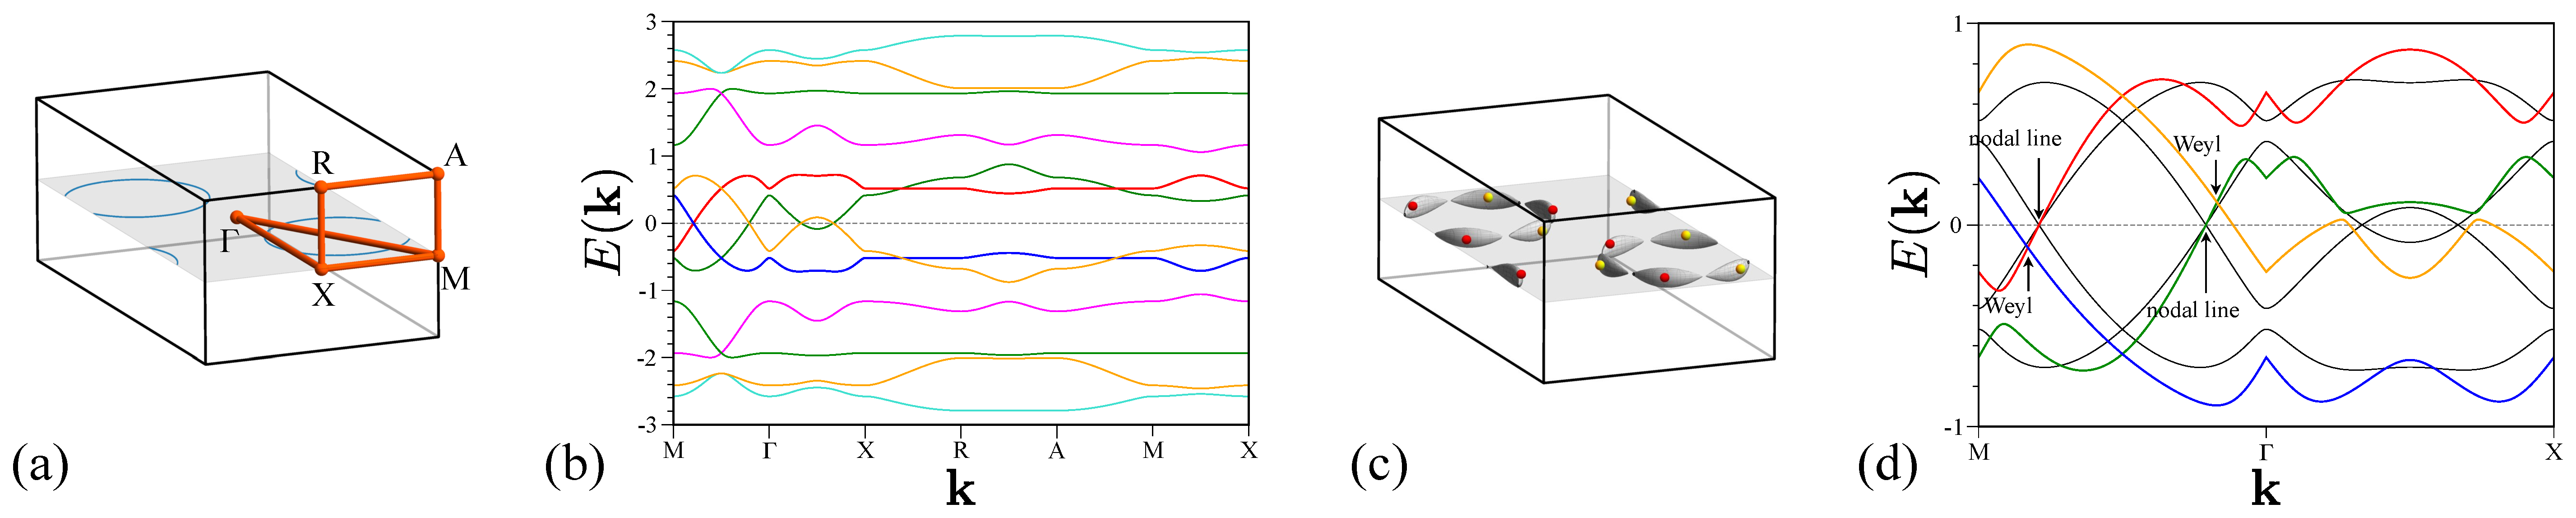
\includegraphics[width=\linewidth]{./chapter05/10_3cPanel2.pdf}
	\caption{
		(a) Brillouin zone of expanded unit cell of lattice (10,3)c with high-symmetry points.
		(b) Majorana dispersion plotted along the high-symmetry paths for $\kappa = 0$.
		(c) Majorana Fermi surfaces for $\kappa = 0.2$ enclosing finite-energy topological degeneracies denoted by red and yellow spheres.
		(d) Majorana dispersion plotted along high-symmetry path.
		The black lines indicates the nodal line dispersion for $\kappa = 0$, whereas, the colored lines indicate the Fermi surface dispersion with topological degeneracies at finite energy for $\kappa = 0.2$.
	}
	\label{fig:chapter05_10_3cPanel2}
\end{figure}
%


%
%
%%%%%%%%%%%%%%%%%%%%%%%%%%%%%%%%%%%%%%%%%%%%%%%%%%%%%%%%%%%%%%%%%%%%%%%%%%%%%%%%%%%%%%%%
\section{Spin-Peierls instabilities}
\label{section:chapter05_SpinPeierls}
%%%%%%%%%%%%%%%%%%%%%%%%%%%%%%%%%%%%%%%%%%%%%%%%%%%%%%%%%%%%%%%%%%%%%%%%%%%%%%%%%%%%%%%%
%
%
While the above discussion focuses solely on the pure Kitaev model, it is necessary to understand the effects of additional interactions, \eg, Heisenberg exchange.
Such additional spin-exchange terms have two generic consequences.
First, they do not commute with the gauge variables, making the gauge field dynamic.
Second, they induce interactions between the itinerant Majorana fermions.
For sufficiently small perturbations, one may ignore the first effect as vison excitations remain gapped.
The effect of interactions, however, depends crucially on the nature of the gapless modes.

For quantum spin liquids with a nodal line or Weyl nodes, a scaling analysis as performed in Reference~\cite{LeePRB2014} shows that the interaction terms are irrelevant in the renormalization group sense.
Thus, such spin liquids are stable against small perturbations.
For quantum spin liquids with a Majorana Fermi surface, however, such interactions are marginal.
A careful analysis~\cite{HermannsPRL2015b} for lattice (10,3)a has shown that time-reversal invariant interactions generically destabilize the Majorana Fermi surfaces even for infinitesimal interaction strength.
In this case, the Fermi surfaces are gapped out with the exception of an odd number of nodal lines.
The following shall serve as a brief review of the underlying mechanism and main features of this instability, which is referred to as a spin-Peierls BCS instability.

As was shown in Section~\ref{section:chapter05_3DKitaevModels}, stable Majorana Fermi surfaces only occur in a pure Kitaev model when the projective time-reversal symmetry is implemented non-trivially, \ie, with non-vanishing $\bk_0$.
Combined with particle-hole symmetry, the result is that the Majorana Fermi surfaces exhibit a perfect nesting, \ie, $E(\bk) = -E(\bk + \bk_0)$.
This perfect nesting is visualized for lattices (10,3)a and (8,3)a in Figure~\ref{fig:chapter05_SpinPeierls}~(a) and (b), respectively.
%
\begin{figure}[tb]
	\centering
	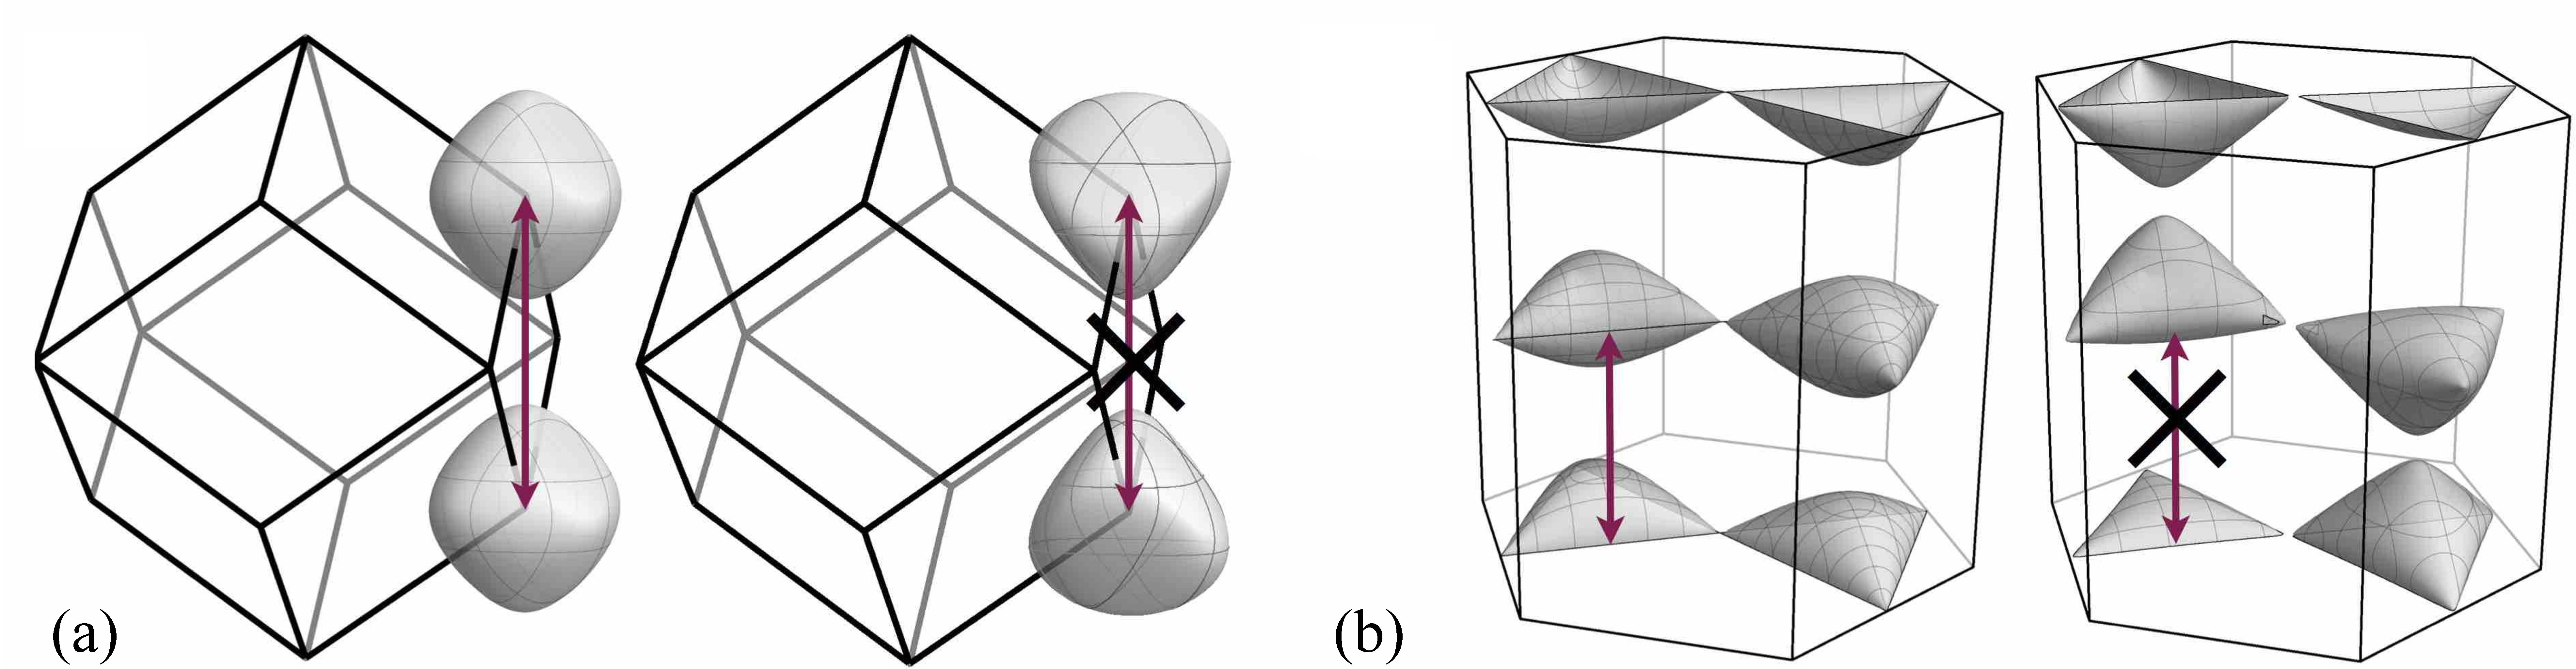
\includegraphics[width=\linewidth]{./chapter05/SpinPeierls.pdf}
	\caption{
		Effects of time-reversal symmetry breaking on (a) lattice (10,3)a and (b) lattice (8,3)a.
		Figures on the left show the time-reversal invariant system, whereas figures on the right show the system with time-reversal symmetry broken for $\kappa = 0.1$.
		Breaking time-reversal symmetry destroys the perfect nesting condition with wave vector $\bk_0$, denoted by the arrow.
	}
	\label{fig:chapter05_SpinPeierls}
\end{figure}
%

It is convenient to express the system in terms of its \textit{complex} fermionic single-particle eigenstates corresponding to the creation/annihilation operators $f_{\alpha}(\bk) = f\dag_{\beta}(-\bk)$.
The $2n$ Majorana Fermi surfaces are then combined into $n$ complex Fermi surfaces and the perfect nesting condition becomes the usual BCS pairing condition $E(\bk_0/2 + \bk) = E(\bk_0/2 - \bk)$ centered around $\bk_0/2$.
Note that there is no $U(1)$ symmetry in this system.
Instead, a non-vanishing pair correlator
%
\begin{equation}
	\avg{f\dag_{\alpha}(\bk_0/2 + \bk) f\dag_{\beta}(\bk_0/2 - \bk)}
\end{equation}
%
breaks translation symmetry spontaneously.
The resulting dimerization is reflected, \eg, in the spin-spin correlations which acquire a staggered component.
Due to the spontaneous breaking of translation symmetry, this BCS-type instability shows similar features to the usual spin-Peierls instability, except that the dimerization occurs for infinitesimal interaction strength.
As shown in Reference~\cite{HermannsPRL2015b}, any time-reversal invariant interaction will, independent of microscopic detail, result in this kind of instability.
For the Kitaev model on lattice (10,3)a, time-reversal symmetry ensures that the Fermi surfaces cannot be gapped out completely and an odd number of nodal lines always remains.
On lattice (8,3)a, however, the presence of \textit{four} rather than two Majorana Fermi surfaces allows, in principle, for interactions to gap the system out entirely.

One way to stabilize the Fermi surfaces is by breaking time-reversal symmetry.
This leads to a deformation of the Fermi surfaces, spoiling the perfect nesting condition (see Figure~\ref{fig:chapter05_SpinPeierls}), \ie, translation by $\bk_0$ in momentum space no longer maps the Fermi surfaces onto each other.
As a result, the BCS instability is cut off at sufficiently low temperatures and the Fermi surface is restored.


%
%
%%%%%%%%%%%%%%%%%%%%%%%%%%%%%%%%%%%%%%%%%%%%%%%%%%%%%%%%%%%%%%%%%%%%%%%%%%%%%%%%%%%%%%%%
\section{Summary and outlook}
\label{section:chapter05_Conclusion}
%%%%%%%%%%%%%%%%%%%%%%%%%%%%%%%%%%%%%%%%%%%%%%%%%%%%%%%%%%%%%%%%%%%%%%%%%%%%%%%%%%%%%%%%
%
%
The work reported in this chapter accomplished several tasks.
First, a number of three-dimensional tricoordinated lattices were considered for the first time in the context of frustrated magnetism.
Second, the Kitaev honeycomb model was investigated for quantum spin-1/2 moments on these lattices with a focus on the gapless spin liquid phase.
Additionally the effects of applying a weak, external magnetic field were considered.
This analysis revealed a rich and varied physics where the low-energy, fermionic quasiparticle excitations formed either full two-dimensional Fermi surfaces, one-dimensional nodal lines or topologically protected Weyl nodes, depending on the lattice under consideration.

Most importantly, this work established a systematic method for classifying and predicting the Fermi surface topology of these Kitaev spin liquids by making use of the projective symmetry group.
The physical symmetry group considered is given by
%
\begin{equation}
SG = \avg{\{ \op{T}_1, \op{T}_2, \op{T}_3, \op{\mathcal{P}}, \op{\mathcal{T}} \}}
\end{equation}
%
and those of its subgroups which include the translation symmetries.
By finding the projective representation of the physical symmetries in a fixed gauge sector, one may identify restrictions that a given projective representation places on the low-energy physics of the model.

The ideas behind this classification, which are scattered throughout the chapter, are now recapitulated below.
With the exception of lattice (10,3)c, the gauge \textit{Ans\"atze} used are all translationally invariant, allowing for the block diagonalization of the Hamiltonian into momentum sectors $H(\bk)$.
Note that such a block diagonalization is also possible for lattice (10,3)c following a doubling of the unit cell.
The projective representations of time-reversal and inversion symmetries lead to the following restrictions of the fermionic quasiparticle spectrum
%
\begin{equation}
	E_{\alpha}(\bk) = E_{\beta}(-\bk + \bk_0) \qquad {\rm and} \qquad E_{\alpha}(\bk) = E_{\gamma}(-\bk + \til{\bk}_0),
\end{equation}
%
where $\bk_0$ and $\til{\bk}_0$ are, in general, distinct superpositions of the reciprocal lattice vectors, \eg, $\bk_0 = (n_1 \bq_1 + n_2 \bq_2 + n_3 \bq_3)/2$ with $n_i \in \{0, 1\}$.
Additionally, the gauge fixed Kitaev Hamiltonian is subject to the particle-hole relation
%
\begin{equation}
	E_{\alpha}(\bk) = -E_{\delta}(-\bk).
\end{equation}
%

For the case that time-reversal symmetry is present \textit{and} its projective representation is trivial, \ie, with $\bk_0 = \bm{0}$, the only stable zero-energy manifolds correspond to one-dimensional nodal lines.
Such nodal lines are seen to be protected by an integer invariant which is well-defined only in the presence of time-reversal symmetry.

When time-reversal symmetry is absent or in the case that its projective representation is \textit{non}-trivial, \ie, with $\bk_0 \neq \bm{0}$, the topology of the nodal manifold depends on the projective representation of inversion symmetry.
If inversion symmetry is absent or its projective representation is non-trivial, \ie, with $\til{\bk}_0 \neq 0$, the only stable zero-energy manifolds correspond to two-dimensional Fermi surfaces.
These Fermi surfaces may be topologically non-trivial in the case that they are a result of topological point-like degeneracies in the spectrum at finite energy or they may be topologically trivial.

When the projective representation of inversion symmetry is trivial, however, such topological point-like degeneracies are fixed to zero energy.
The result is that the only stable zero-energy manifolds correspond to zero-dimensional Weyl nodes, \ie, gapless excitations correspond to massless, chiral fermions.
An interesting consequence of symmetries being represented projectively in the Majorana sector is the possibility of stable Weyl nodes in the presence of \textit{both} time-reversal and inversion symmetries -- a situation which is \textit{not} possible in conventional, electronic Weyl semi-metals.

In the cases that the projective symmetries induce a shift in the momentum space relations, \eg, when $\bk_0 \neq \bm{0}$, the resulting nodal manifold is necessarily doubled and subject to a perfect nesting condition.
This results in an instability for those lattices exhibiting a fully two-dimensional Fermi surface in the presence of interactions.
This so-called spin-Peierls BCS instability may be neutralized, however, by breaking the symmetry which is responsible for the nesting vector.

Finally, it should be repeated that the analyses of lattices (8,3)c and (9,3)a were not performed in the ground state flux sector.
In both cases, subsequent quantum Monte Carlo studies have been undertaken to determine the flux configurations throughout the entire ground state phase diagram.
Reference~\cite{EschmannPRL2019}, which reports a detailed study of the Kitaev model on lattice (8,3)c, similarly finds nodal lines for roughly isotropic couplings as expected from the analysis of this chapter.
A more realistic analysis of the Kitaev model on lattice (9,3)a is the subject of Chapter~\ref{chapter:HypernonagonLattice}.